
\input{../header}

\hypersetup{
 	pdftitle={01MAS - Matematická statistika},
 	pdfauthor={WIKI Skripta},
 	pdfsubject={Zápisky z~přednášek MAS, FJFI ČVUT},
 	pdfkeywords={matematická statistika},
 	bookmarksnumbered=true,
 	colorlinks=true,
 	pdfpagemode={UseOutlines}
 }
\makeindex
 
\title{01MAS Matematická statistika}
\date{\today}
\author{Martin Kovanda\\(revize a~korektury Václav Kůs)}
 
\begin{document}

% ****************************************************************************************************************************
%                             FRONTMATTER
% ****************************************************************************************************************************
\frontmatter
\maketitle
 
\newpage
\pdfbookmark[0]{Obsah}{obsah}
\tableofcontents
 
%\wikiskriptum{01DIFRnew}
% ****************************************************************************************************************************
%                             KAPITOLA: Předmluva
% ****************************************************************************************************************************
\chapter*{Předmluva}
\pdfbookmark[0]{Předmluva}{predmluva}

Materiál byl původně sestavován na~základě přednášek Ing. Václava Kůse, Ph.D., které proběhly v~letním semestru akademického roku 2019/2020 na~Fakultě jaderné a~fyzikálně inženýrské ČVUT v~Praze. Vzhledem k~probíhající pandemii Covid-19 však byla přerušena kontaktní výuka, a~proto byl zbytek materiálů vytvořen přepracováním zápisků z~tabule z~akademického roku 2018/2019. Tímto bych chtěl poděkovat Ing. Václavu Kůsovi, Ph.D., za~rozsáhlou korekturu a~doplnění materiálů, bez~kterého by se~tato práce neobešla. Dále bych chtěl poděkovat všem, kteří v~této práci našli chyby a~upozornili na~ně, případně je i~opravili.\\ ~\\
Zároveň tímto vyzývám čtenáře, aby podobným způsobem zpracovali další předměty. Tvorba těchto materiálů zabere hodně času a~usilí, ale dle mého názoru má veliký smysl pro~všechny, kteří budou tento předmět navštěvovat. \\~\\
Tento učební text je určen posluchačům 3.~ročníku základního studia navštěvujícím kurs 01MAS \emph{Matematická statistika}, který je zařazen 
mezi předměty oborů AMSM a~MM. Při~sestavování textu se~předpokládaly znalosti základů matematiky na~úrovni absolvování kurzů 01MAB2-4, 01LAB1-2 a~01MIP.

~

%\textbf{Doporučená literatura:}
%\begin{enumerate}[(1)]
%  \item 
  
%\end{enumerate}
 
%Diferenciální rovnice navazují na~kurz lineární algebry a~matematická analýzy. Na~tento předmět budou v~dalších semestrech navazovat:
%\begin{enumerate}
%  \item 01SEDR --- Seminář diferenciálních rovnic (náplní geometrická teorie diferenciálních rovnic)
%  \item 01MMNS --- Matematické modelování nelineárních systému
%  \item 01MMF --- Metody matematické fyziky (náplní parciální diferenciální rovnice)
%\end{enumerate}



% ****************************************************************************************************************************
%                             MAINMATTER
% ****************************************************************************************************************************
\mainmatter
\chapter{Statistika - setup a~základní postupy}
Představme si, že máme nějakou reálnou situaci a~chceme na~ní vytvořit statistický matematický model, který závisí na~jistých parametrech ($\t$). Narozdíl od~jiných předmětů ale máme k~dispozici výsledky měření z~navrženého experimentu a~zkoumáme jejich příčinu. Máme opět $\prostor$. $\Omega$ zde nazveme \textbf{populace}, $\omega\in\Omega$ nazveme \textbf{individuum}. 

Náhodná veličina $X:\Omega\to\R$ zde bude představovat \textbf{vlastnost} zkoumanou na~dané populaci $\Omega$ (např. počet špatných výrobků v~sérii). Tuto vlastnost zjišťujeme experimentálně, např. měřením, vážením apod. Víme také, že $X\sim\PP^X$ má jisté rozložení na~$\prostor$ dané např. pomocí  $\FF_X,f_X,p_X,...$, které ale neznáme a~chceme ho zjistit. 
\begin{define}
	n-tici nezávislých náhodných veličin $X_1,...,X_n$ stejně rozdělených s~distribuční funkcí $\FF$ nazýváme \textbf{náhodný výběr} z~rozdělení $\FF$. Konkrétní realizací $\X$ získáme vektor čísel $\textbf{x}=(x_1,...,x_n)$, který nazveme \textbf{realizace} náhodného výběru $X_1,...,X_n$, neboli naměřená data.
\end{define}
\begin{example}
	Příkladem je třeba $n$ opakování stejných experimentů, ve~kterých máme pokaždé stejné nastavení. Používáme tedy stejnou metodu měření. Dalším příkladem může být $n$ výrobků z~nějaké dodávky zboží, na~základě kterých určujeme celkový počet zmetků.
\end{example}

\begin{define} 
	Vybereme vektor individuí $\omega^{(n)}=(\omega_1,...,\omega_n)\in\Omega^n$ a~definujeme $$X_j\br{\omega^{(n)}}:=X(\omega_j),~\forall j\in\hat{n},$$ jako \textbf{pozorování} (v tomto tvaru máme skutečná data). Zavedeme dále $\Omega^{(n)}:=\Omega^n,$\newline$\Aa^{(n)}:=\sigma(\Aa^n)$, $\PP^{(n)}:=\bigotimes\limits_{1}^n \PP^X$ (součinová míra), tedy $$ \PP^{(n)}(A_1\times ...\times A_n)=\prod\limits_{j=1}^n \PP^X(A_j),~\forall A_j\in\Aa .$$
\\ \\
 Definujeme
	\textbf{realizaci} náhodného výběru $\X=(X_1,...,X_n)$ vztahem $$\textbf{x}=\X(\omega^{(n)}).$$
\end{define}

\begin{theorem}\label{iid}
	$\poslkon~iid~\PP^X$.
	\begin{proof} Pro~$\forall B\in\Bb$ a~$\forall j \in\widehat{n}$ platí, že 
		$$ \PP^{X_j}(B)=\PP^{(n)}\circ \inv{X_j}(B)=\PP^{(n)}\br{\underbrace{\{ X_j\in B \}}_{\Omega\times\Omega...\times\{ X\in B \}\times \Omega...}}=\PP(X\in B)=\PP^X(B). $$ Zbývá nám ještě dokázat nezávislost:
		$$ \PP^{(n)}\Br{\bigcap\limits_{j=1}^n\{ X_j\in B_j \}}=\PP^{(n)}\Br{\bigtimes\limits_{j=1}^n\{ X\in B_j \}}=\prod\limits_{j=1}^n\PP(X\in B_j)=\prod\limits_{j=1}^n\PP^{(n)}(X_j\in B_j), $$ protože $B_j$ jsou pokaždé na~jiné "pozici" v~kartézském součinu $\Omega\times...\times\{ X\in B_j \}\times...\times\Omega$.
	\end{proof}
\end{theorem}
\begin{define}
		\textbf{Statistika} je libovolná funkce náhodného výběru $X_1,...,X_n$, jejíž funkční předpis nezávisí na~parametrech příslušného rozdělení.
		\\ \\
	Příkladem statistiky může být \textbf{výběrový průměr} (sample mean)$$\Oxn=\frac{1}{n}\sumjn X_j,$$ případně \textbf{geometrický průměr}
	$$ \Oxn^G=\sqrt[n]{X_1X_2...X_n}, $$\textbf{výběrový rozptyl}
	$$ \hsn=\frac{1}{n}\sumjn(X_j-\Oxn)^2\text{ \quad nebo\quad  }s_n^2=\frac{1}{n-1}\sumjn (X_j-\Oxn)^2,$$ kde $\widehat{\sigma}_n$ nebo případně $s_n$ je \textbf{výběrová směrodatná odchylka}. Dále uveďme \textbf{$r$-tý výběrový obecný a~centrální moment} (sample moments)
	$$m_r'=\frac{1}{n}\sumjn X_j^r,\qquad m_r=\frac{1}{n}\sumjn(X_j-\Oxn)^r,$$ 
	\textbf{medián}
	$$ \widehat{X}_{\frac{1}{2}} = \begin{cases}
	X_{(\frac{n+1}{2})} & n\text{ liché}, \\ \frac{1}{2}\br{X_{(\frac{n}{2})}+X_{(\frac{n}{2}+1)}} & n\text{ sudé},
	\end{cases} $$  kde $X_{(j)}$ značí $j$-tou zdola uspořádanou statistiku z~náhodného výběru $\br{X_{(1)}\leq...\leq X_{(n)}}$.
\end{define}



\section{Statistické bodové odhady}
Nechť $\t$ je parametr spojený s~rozdělením $\PP^X$, tzn. $\t=\t(\PP^X)$. Máme dvě možnosti. 
\begin{enumerate}[a)]
	\item $\t$ může být spojený s~$\PP^X$, např. $\t=\E X,\D X, \FF_X(t),...$, nebo
	\item $\t$ může být přímo parametr rozdělení $\PP_\t^X$.
\end{enumerate}
V obou případech ale požadujeme tzv. identifikovatelnost rodiny $\mathcal{P}=\{\PP^X\}$, resp.\\ $\mathcal{P}=\{\PP_\t^X:\t\in\Theta\}$, tzn., že každému parametru přísluší právě jedna pravděpodobnost $X$.
$$ \t_1\neq\t_2~\Rightarrow~\PP_1^X\neq\PP_2^X,\quad\text{resp.}\quad \t_1\neq \t_2 \Rightarrow P_{\t_1}^X\neq P_{\t_2}^X.$$
Opačná implikace často neplatí, třeba pro~danou střední hodnotu najdeme vícero různých rozdělení.
Předpokládáme, že $\t\in\Theta\subset \R^k$, kde $\Theta$ se~nazývá \textbf{parametrický prostor}. Dále máme $\tau(\t):\Theta\to\R^s$, kde $\tau$ je tzv. \textbf{parametrická funkce} (většinou nás ale zajímá např. jedna vybraná složka, tedy $s=1$). Odhadnout celé rozdělení se~nám většinou nepodaří (nebo to nepotřebujeme), proto hledáme odhad parametru $\t$. 

\begin{define}
	Libovolná (borelovsky) měřitelná funkce náhodného výběru $X_1,...,X_n$ (tedy statistika) \[
	\begin{split}
	\htn(\X)&:\Omega^n\to\R^k\text{ se~nazývá \textbf{odhadem} (estimator) }\t\in\Theta\subset\R^k. \\
	\widehat{T_n}(\X)&:\Omega^n\to\R^s\text{ se~nazývá \textbf{odhadem} (estimator) parametrické funkce }\tau(\t)\in\tau(\Theta)\subset\R^s.
	\end{split}
	\] 
\end{define}
\begin{remark}
	Tato definice nám však neříká, jak tuto statistiku volit. Aby však poskytovala námi žádané výsledky, je potřeba, aby splňovala některé vlastnosti.
\end{remark}

\section{Vlastnosti bodových odhadů}
\begin{define}
	$T_n(\X)$ nazýváme \textbf{nestranný odhad} $\tau(\t)$, pokud $$\E_\t T_n(\X)=\tau(\t),~\forall\t\in\Theta,~\forall n\in\N.$$  
	$T_n(\X)$ nazýváme \textbf{asymptoticky nestranný odhad} $\tau$, pokud $$\E_\t T_n(\X)\to\tau(\t),~\forall\t\in\Theta,$$
	kde $\E_\t$ značí střední hodnotu vzhledem k~rozdělení $\PP_\t^X$.
\end{define}
\begin{remark}
	Střední hodnotu tedy chápeme jako "průměrování" přes všechny možné výběry, které lze získat pod~rozdělením $\PP_\t^X$ při~daném fixním, ale libovolném $\t$.
\end{remark}

\begin{define}
	$T_n(\X)$ nazýváme \textbf{eficientní} (vydatný), pokud pro~$\forall\widetilde{T}_n,~\forall\t\in\Theta$ platí \[
	\begin{split}
	s=1:~&\E\Big[\br{T_n(\X)-\tau(\t)}^2\Big]\leq \E\Big[\br{\widetilde{T}_n(\X)-\tau(\t)}^2\Big], \\
	s>1:~&\E\Big[\nor{T_n(\X)-\tau(\t)}_{\epsilon}^2\Big]\leq \E\Big[\nor{\widetilde{T}_n(\X)-\tau(\t)}_{\epsilon}^2\Big].
	\end{split}
	\]  
	$\E(T_n-\tau)^2$ se~nazývá střední kvadratická chyba - MSE (\textit{mean squared error}) odhadu $T_n(\X)$. Tedy eficientní odhad má nejnižší možnou MSE. Pro~nestranné odhady $\br{\tau(\t)=\E T_n(\X)}$ tento vztah pro~$s=1$ přechází na~$\D T_n(\X)\leq \D \widetilde{T}_n(\X)$.
\end{define}

\begin{define}
	Máme-li $T_n^1,T_n^2:\Omega\to\R^1$ jako odhady $\tau(\t)$, pak definujeme \textbf{relativní eficienci} vztahem $$\RE=\frac{\E(T_n^1-\tau)^2}{\E(T_n^2-\tau)^2}\equal{\text{nestranný odhad}}\frac{\D T_n^1}{\D T_n^2}.$$
\end{define}


Zkusme nyní porovnat dvě statistiky tak, abychom určili, která z~nich je lepší. Pokud porovnáváme 2 nestranné statistiky, pak lepší (\textbf{vydatnější}) z~nich je ta s~menším rozptylem. Pokud však porovnáváme statistiky, které nejsou nestranné, pak nutně nemusí být lepší ta s~nižším rozptylem. Používáme k~tomu tedy právě definovanou \textbf{MSE} (střední kvadratickou odchylku, mean squared error) (viz obrázek \ref{fig:mse}) $$ \MSE(\hat{\t})=\E(\hat{\t}-\t)^2,\text{ kde $\hat{\t}$ je odhadem neznámého parametru $\t$.} $$
\begin{figure}[h]
	\centering
	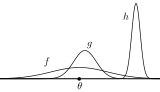
\includegraphics[width=0.4\linewidth]{Images/MSE}
	\caption{Ukázka toho, že statistika s~nejmenším rozptylem (h) nebo s~nejbližší střední hodnotou (f) nemusí být nutně ta nejvhodnější.}
	\label{fig:mse}
\end{figure}

\begin{define}
	$T_n(\X)$ se~nazývá \textbf{konzistentní} odhad $\tau$, pokud $$T_n(\X)\PSJ\tau(\t),\quad\forall\t\in\Theta$$ (pro $\Pto$ slabě konzistentní, pro~$\sj$ silně konzistentní).
\end{define}

\begin{theorem}[Kritérium konzistence]
	Odhad $T_n(\X)$ je slabě konzistentní $(T_n(\X)\Pto\tau(\t))$, pokud \begin{enumerate}
		\item $T_n(\X)$ je asymptoticky nestranný $(\E_\t T_n(\X)\to\tau(\t),$ pro~$\forall\t\in\Theta)$ a
		\item platí pro~něj, že $\D T_n(\X)\to0$.
	\end{enumerate}
\end{theorem}

\begin{example}
	Statistika je funkce náhodných veličin, a~proto se~taky chová jako náhodná veličina. Má proto taky své vlastní rozdělení a~například střední hodnota jejího rozdělení nám může poskytnout užitečné informace. Příkladem je zkoumání realizace exponenciálního rozdělení $\Exp(\frac{1}{2})$ (viz obr. \ref{fig:hist0}). Vezměme nyní statistiku "výběrový průměr" (výběrová střední hodnota). Na~obrázku \ref{fig:hist1} vidíme, že střední hodnota výběrového průměru odpovídá $\mu=\frac{1}{2}$, což je důsledek toho, že je statistika nestranná. Pro~vyšší $n$ jde zároveň její rozptyl k~nule. Tyto vlastnosti vyplývají z~centrální limitní věty, která říká, že výběrový průměr má přibližně normální rozdělení (pro data z~normálního rozdělení pak přímo normální rozdělení) dané vztahem
	$$ \Oxn\sim\AN\Br{\mu,\frac{\sigma^2}{n}}. $$
	%http://www.karlin.mff.cuni.cz/~hudecova/education/download/chem_predn/nahodny_vyber_tisk.pdf
	\begin{figure}[h]
		\centering
		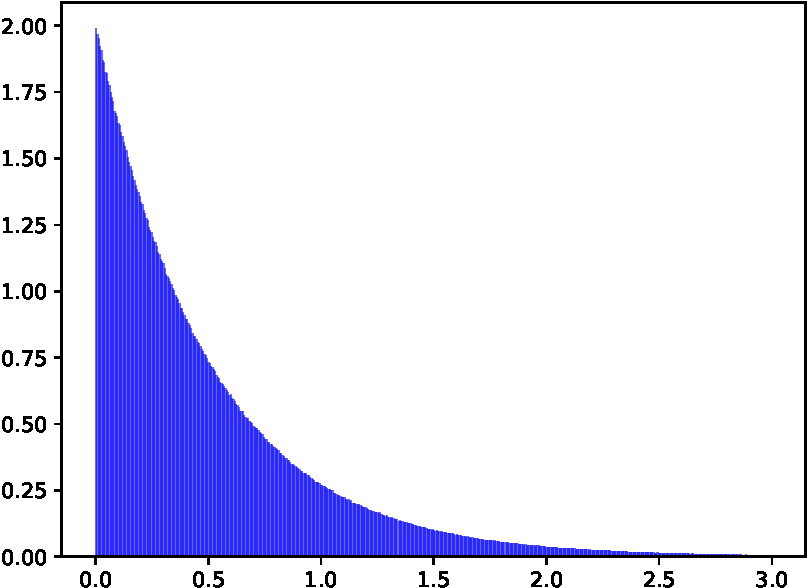
\includegraphics[width=0.3\linewidth]{Images/histexp0}
		\caption{Hustota pravděpodobnosti rozdělení $\Exp(\frac{1}{2})$.}
		\label{fig:hist0}
	\end{figure}
	
	\begin{figure}[h]
		\centering
		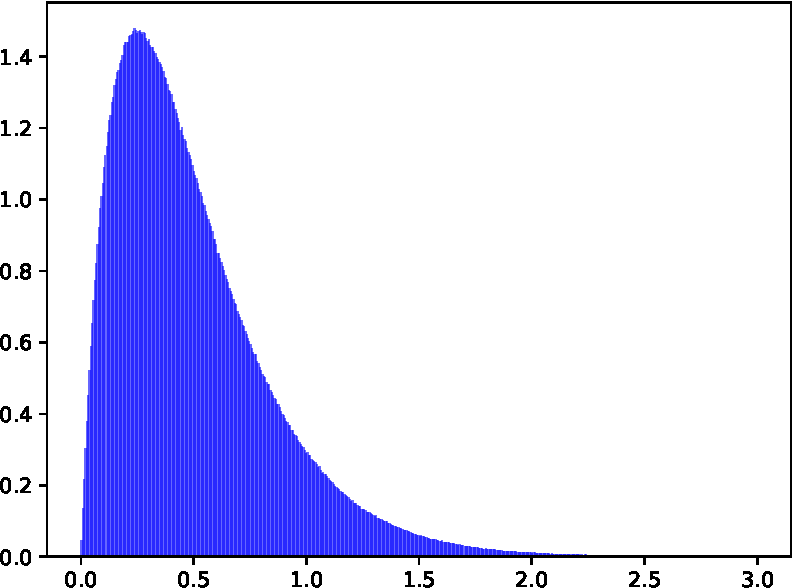
\includegraphics[width=0.32\linewidth]{Images/histexp2}
		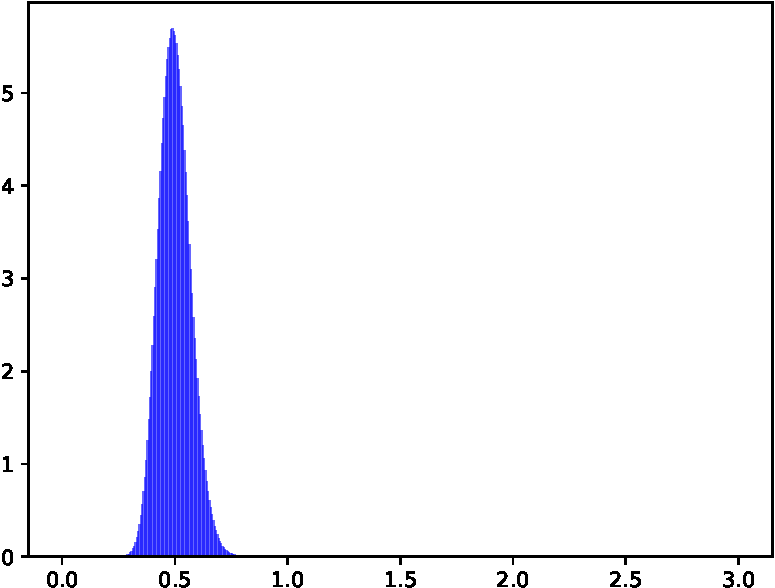
\includegraphics[width=0.32\linewidth]{Images/histexp50}
		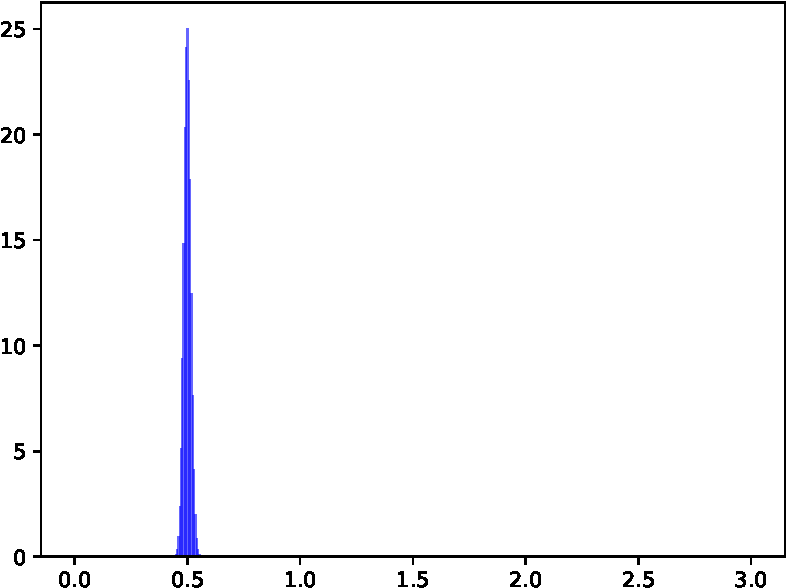
\includegraphics[width=0.32\linewidth]{Images/histexp1000}
		\caption{Hustota pravděpodobnosti výběrového průměru pro~$n=2,~n=50$ a~$n=1000$. Vidíme tedy, že $\Oxn\sim\AN\Br{\mu,\frac{\sigma^2}{n}}$, kde $\mu=0.5$.}
		\label{fig:hist1}
	\end{figure}
\end{example}
\begin{define}
	$T_n(\X)$ se~nazývá \textbf{asymptoticky normálním} odhadem $\tau(\t)$ s~asymptotickou kovarianční maticí $\C(\t)$ (matice tvaru $s\times s$), pokud pro~$\forall\t\in\Theta$ $$ T_n(\X)\sim\AN_s\Br{\tau(\t),\frac{1}{n}\C(\t)}\text{, tzn. \quad } \sqrt{n}\br{T_n(\X)-\tau(\t)}\Dto \NN _s\br{\textbf{0},\C(\t)}\text{ (viz CLT)}. $$
	\\ \\
	Pro $s=1$ definice přechází na~$\sqrt{n}\br{T_n(\X)-\tau(\t)}\Dto \n{0,\sigma^2(\t)}$, kde $\sigma^2(\t)$ nazýváme asymptotický rozptyl odhadu $T_n(\X)$. 
\end{define}

\begin{define}
	Máme-li $T_n^1,T_n^2$ jako odhady $\tau(\t)$, které jsou oba $\AN$ odhady $\tau$ s~asymptotickými rozptyly $\sigma_1^2(\t)$ a~$\sigma_2^2(\t)$, pak definujeme \textbf{asymptotickou relativní eficienci} vztahem $\ARE=\frac{\sigma_1^2(\t)}{\sigma_2^2(\t)}$.
\end{define}

\begin{remark}
	\begin{itemize}
		\item Odtud nutně neplyne, že $\E\Br{\sqrt{n}\br{T_n(\X)-\tau(\t)}}\to 0 $ (tedy asymptotická nestrannost $T_n$), protože $\lim\limits_{n\to+\infty}\E T_n$ nemusí nutně existovat.
		\item Nemusí dokonce platit ani vztah $\D\Br{\sqrt{n}\br{T_n(\X)-\tau(\t)}}=\D\Br{\sqrt{n}\br{T_n(\X)}}\to\sigma^2(\t)$. (rovnítko vyplývá z~posunutí o~konstantu).
	\end{itemize}
\end{remark}

\begin{theorem}
	$T_n(\X)$ je asymptoticky normální $\AN\Br{\tau(\t),\frac{1}{n}\sigma^2(\t)}$. Pak $T_n(\X)\Pto\tau(\t),~\forall\t\in\Theta$. 
Tato slabá konzistence je řádu $o_p(n^{-\alpha}),~\alpha<\frac{1}{2}$, tzn., že $n^\alpha(T_n(\X)-\tau(\t))\Pto0,~\forall\alpha<\frac{1}{2}$. To vyplývá z~věty (MIP) $\Br{\text{Mějme }\posln,~X_n\sim\AN(\mu,\sigma_n^2)\text{ tak, že }\sigma_n\to 0.\text{ Pak }X_n\Pto \mu.}$.
\end{theorem}

\begin{theorem}[$\Delta$-metoda]\label{lamatko}
	Nechť $T_n(\X)\sim\AN\Br{\tau(\t),\frac{1}{n}\sigma^2(\t)}$ a~$g:\R^1\to\R^1$ spojitě diferencovatelnou v~$\tau(\t),~\forall\t\in\Theta$. Pak $$g\br{T_n(\X)}\sim\AN_1\left( g\br{\tau(\t)},\frac{\sigma^2(\t)}{n}\left[ g'\br{\tau(\t)} \right]^2 \right).$$
\end{theorem}
\begin{example}
	Například pokud $T_n(\X)=\Oxn,~g(t)=t^2,~g'(t)=2t$, pak$$ (\Oxn)^2\sim\AN(\mu^2,\frac{\sigma^2}{n}\cdot 4\mu^2). $$ 
	\begin{figure}[h]
		\centering
		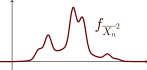
\includegraphics[width=0.3\linewidth]{Images/fxn1} \raisebox{5.6ex}{$\stackrel{n\to+\infty}{\longrightarrow}$}
		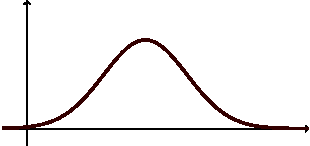
\includegraphics[width=0.3\linewidth]{Images/fxn2}
		\label{fig:fxn1}
	\end{figure}
\end{example}
\section{Výběrové charakteristiky a~jejich vlastnosti}
\begin{theorem}
	Mějme $X\in\LL_1$, resp. $\LL_2$, volme $\t=\t(\PP^X)=\E X=\mu$ a~označme \\$\sigma^2=\D X<+\infty~(\LL_2)$. Pak \textbf{sample mean} $$T_n(\X)=\Oxn=\frac{1}{n}\sumjn X_j$$ je nestranným, konzistentním a~$\AN\Br{\E X,\frac{1}{n}\sigma^2}$ odhadem $\t=\E X=\mu$.\begin{proof}Víme, že $X_1,...,X_n$ jsou $iid$ podle věty \ref{iid}. Pak
		\begin{enumerate} 
			\item $\E \Oxn=\mu,~\forall\mu$,
			\item $\Oxn\PSJ\E X$, což platí díky~ZVČ (Kolmogorov 2, kde požadujeme $\poslkon~iid ~\LL_1$),
		\end{enumerate}
	\end{proof}
\end{theorem}
\begin{remark}
	\begin{enumerate}
		\item CLT$_{L-L}$: $\Oxn\sim\AN\Br{\mu,\frac{\sigma^2}{n}}$ (zde požadujeme $\poslkon~iid~\LL_2$).
		\item 	$X$ zde značí vlastnost na~$\Omega$ a~$\X=(X_1,...,X_n)$ je náhodný výběr. Není to tedy realizace!
	\end{enumerate}

\end{remark}
\begin{theorem}
	$X\in\LL_2$, resp. $\LL_4$, volme $\t=\t(\PP^X)=\D X=\sigma^2$. Pak \textbf{výběrový rozptyl} $$T_n(\X)=\hsn=\frac{1}{n}\sumjn(X_j-\Oxn)^2\text{ \quad i\quad  }T_n(\X)=s_n^2=\frac{1}{n-1}\sumjn(X_j-\Oxn)^2$$ jsou oba asymptoticky nestranné, konzistentní a~$\AN\Br{\sigma^2,\frac{1}{n}(\mu_4-\sigma^4)}$ odhady $\sigma^2$, kde\\ $\mu_4=\E\left[ (X-\E X)^4 \right]$.
	V případě $T_n(\X)=s_n^2$ je $T_n(\X)$ navíc nestranný odhad $\sigma^2,~\forall n\in\N$.
	\begin{proof}Konzistence:
		$$ \hsn=\frac{1}{n}\sumjn(X_j-\Oxn)^2=\frac{1}{n}\sumjn X_j^2-\frac{2}{n}\sumjn X_j\Oxn+\Oxn^2=\underbrace{\frac{1}{n}\sumjn X_j^2}_{\overline{Y_n}\PSJ \E Y_1=\E X^2}-\underbrace{\Oxn^2}_{\to(\E X)^2}\PSJ \D X $$
		Nestrannost (pro $\hsn$ pouze asymptotická):
		\[
		\begin{split}
		\E\br{\hsn}&=\E \Br{\frac{1}{n}\sumjn X_j^2-(\Oxn)^2}=\E X^2-\E(\Oxn^2)=\E X^2-\frac{1}{n^2}\E\Br{\sumjn X_j^2-\sum\limits_{i\neq j}^nX_iX_j}=\\&=\E X^2-\frac{1}{n}\E X^2-\frac{1}{n^2}n(n-1)(\E X)^2=\frac{n-1}{n}\underbrace{\left[ \E (X^2)-(\E X)^2 \right]}_{=\D X=\sigma^2} =\frac{n-1}{n}\sigma^2\to \sigma^2,
		\end{split}
		\]
		$$ \E s_n^2=\frac{n}{n-1}\E \widehat{\sigma}_n^2=\sigma^2. $$ Asymptotická normalita $\hsn$ i~$s_n^2$ plyne z~rozkladu $\hsn=\frac{1}{n}\sumjn(X_j-\mu)^2-(\Oxn-\mu)^2$ a~ze~Slutskyho lemma.
	\end{proof}
\end{theorem}
\begin{remark}
	V případě dat \ref{fig:hist0}, kde $\sigma^2=0.25$ je situace zachycena na~obrázku \ref{fig:hist2}.
	
\end{remark}
\begin{dusl}
	Mějme $X\in\LL_2$.	Potom pro~tzv. \textbf{t-statistiku} platí, že $$t_n=t_n(\X)=\frac{\sqrt{n}(\oxn-\mu)}{s_n}\Dto\NN(0,1).$$\begin{proof}
		Z CLT$_{L-L}$	$$ \sqrt{n}(\Oxn-\mu)\Dto\NN(0,\sigma^2),\quad s_n\PSJ\sigma. $$
		Podíl tedy konverguje v~distribuci (Slutsky),
		$$ \frac{\sqrt{n}(\Oxn-\mu)}{s_n}\Dto\frac{\NN(0,\sigma^2)}{\sigma}=\NN(0,1). $$
	\end{proof}	\begin{figure}[h]
		\centering
		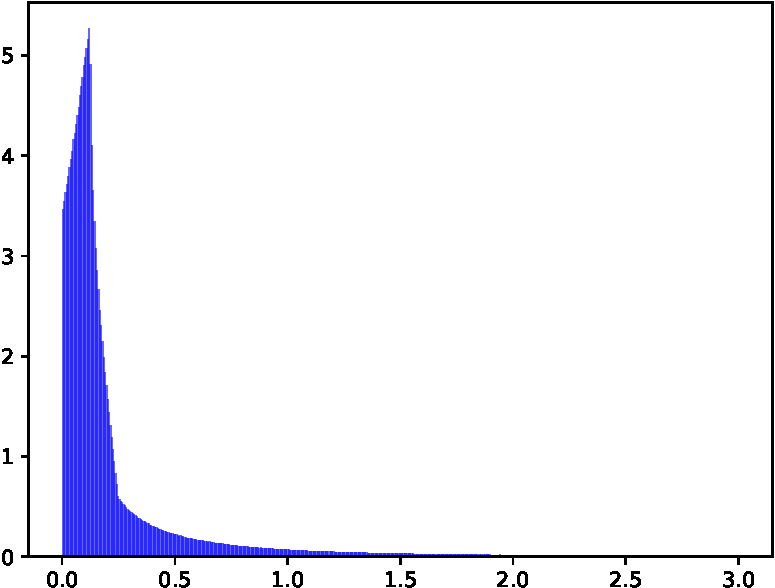
\includegraphics[width=0.32\linewidth]{Images/histexp_var2}
		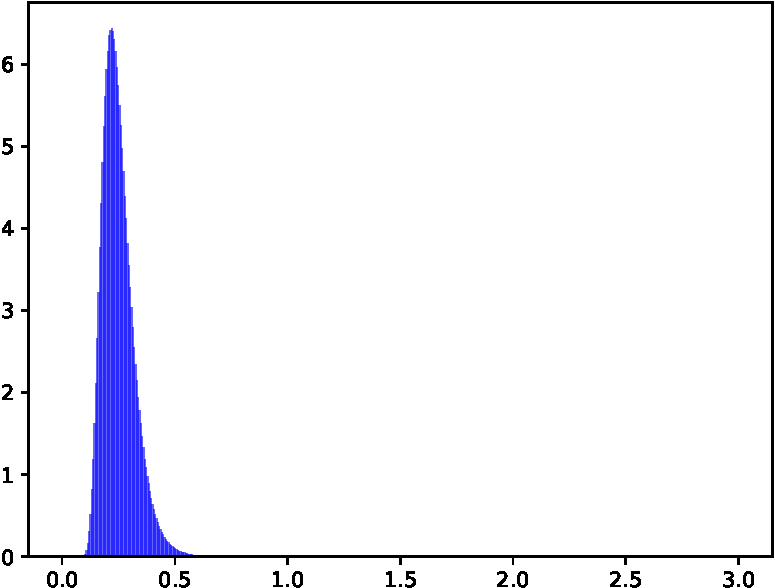
\includegraphics[width=0.32\linewidth]{Images/histexp_var100}
		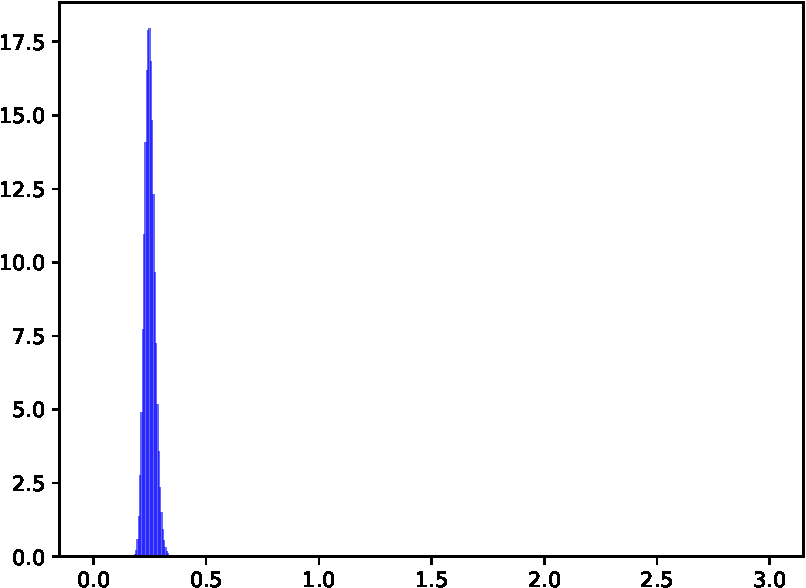
\includegraphics[width=0.32\linewidth]{Images/histexp_var1000}
		\caption{Histogram výběrového rozptylu realizace \ref{fig:hist0} (10000000 rozptylů) pro~$n=2$, $n=100$ a~$n=1000$. }
		\label{fig:hist2}
	\end{figure}
\end{dusl}

\begin{theorem}[Chinčin]
	Mějme $X\in\LL_r$, resp. $X\in\LL_{2r},~r\geq 1$, volíme $$\t_1=\t_1(\PP^X)=\E(X^r)=\mu'_r,\qquad\t_2=\E(X-\E X)^r=\mu_r.$$ Pak $r$-tý výběrový moment
	$$m_r'=m_r'(\X)=\frac{1}{n}\sumjn X_j^k$$
	je nestranným, konzistentním a~$\AN$ odhadem $\t_1=\mu'_1$ a~ $$m_r=m_r(\X)=\frac{1}{n}\sumjn(X_j-\oxn)^r$$ je konzistentním odhadem $\mu_r$.
\end{theorem}

\begin{theorem}Speciálně nyní mějme $(X_j)_{j=1}^{n,+\infty}~iid~\n{\mu,\sigma^2}$. Pak \begin{enumerate}[a)]
		\item $\Oxn\sim\n{\mu,\frac{\sigma^2}{n}},~\forall n\in\N$. Dále potom $\E \Oxn=\mu$, $\D\Oxn=\sigma^2$, $\frac{\sqrt{n}(\oxn-\mu)}{\sigma}\sim\n{0,1}$,
		\item $\hsn=\frac{1}{n}\sumjn(X_j-\Oxn)^2\quad \stackrel{\NN}{\Rightarrow}\quad \frac{n\hsn}{\sigma^2}\sim\chi^2(n-1),~\forall n\in\N$ (Pearsonovo rozdělení).\newline
		$s_n^2=\frac{1}{n-1}\sumjn(X_j-\Oxn)^2\quad \stackrel{\NN}{\Rightarrow}\quad \frac{(n-1) s_n^2}{\sigma^2}\sim\chi^2(n-1),~\forall n\in\N$. Dále platí
		\[
		\begin{split}
		\D(\hsn)&=\frac{\sigma^4}{n^2}2(n-1)=\frac{n-1}{n^2}(2\sigma^4)\to 0, \\
		\D(s_n^2)&=\D\left( \frac{\sigma}{n-1}\chi^2(n-1) \right)=\frac{\sigma^4}{(n-1)^2}2(n-1)=\frac{2\sigma^4}{n-1}\to0, \\
		\D(s_n^2)&>\D(\hsn).
		\end{split}
		\]
		\item $\Oxn$ a~$s_n^2$ jsou nezávislé a~platí 
		$$ \frac{\sqrt{n}(\oxn-\mu)}{s_n}=\frac{\frac{\sqrt{n}(\oxn-\mu)}{\sigma}}{\frac{s_n}{\sigma}}\sim\frac{\n{0,1}}{\sqrt{\frac{\chi^2(n-1)}{n-1}}}\sim t(n-1),~\forall n\in\N \text{ (Studentovo rozdělení).}$$
		\item Pokud jsou $X,Y$ na~$\prostor$ nezávislé, pak pro
		\begin{align*}
		&X_1,...,X_n~iid~\n{\mu_1,\sigma_1^2}\text{, ze~kterých známe } \Oxn,s_{1,n}^2, \\
		&Y_1,...,Y_m~iid~\n{\mu_2,\sigma_2^2}\text{, ze~kterých známe }  \overbar{\rule{0ex}{1.8ex}Y_m},s_{2,m}^2,
		\end{align*} platí, že 
		$$ \frac{s_{1,n}^2(n-1)}{\sigma_1^2}\sim\chi^2(n-1),\qquad \frac{s_{2,m}^2(m-1)}{\sigma_2^2}\sim\chi^2(m-1). $$
		Navíc lze ukázat, že $s_{1,n}^2$ a~$s_{2,m}^2$ jsou nezávislé.
	\end{enumerate}
\end{theorem}
\begin{dusl}
	$$ T_n(\X)=\frac{\frac{s_{1,n}^2}{\sigma_1^2}}{\frac{s_{2,m}^2}{\sigma_2^2}}=\frac{\frac{\chi^2(n-1)}{n-1}}{\frac{\chi^2(m-1)}{m-1}}\sim\FF(n-1,m-1)\quad\text{(Fisherovo rozdělení).} $$
\end{dusl}

\section{Výběrový kvantil (a jeho vlastnosti)}
\begin{define}
	Mějme náhodný výběr $(X_1,...,X_n)$. Pak $\left( X_{(1)},...,X_{(n)} \right)$ nazveme \textbf{uspořádaný náhodný výběr} (vzestupně). \textbf{Výběrový $\alpha$-kvantil} definujeme jako $\widehat{X}_{\alpha,n}=X_{([\alpha n]+1)} $, pro~$\alpha=\frac{1}{2}$ nazýváme $\widehat{X}_{\frac{1}{2}}$ \textbf{výběrovým mediánem}, který alternativně označujeme jako $\widehat{X}_\txt{med}$. \textbf{Výběrové rozpětí} pak definujeme jako $d=X_{(n)}-X_{(1)}$ a~\textbf{výběrové interkvartilové rozpětí} jako $$d_{\frac{1}{4}}=X_{\left( \left[\frac{3}{4}n\right]+1 \right)}-X_{\left( \left[\frac{1}{4}n\right]+1 \right)}.$$
\end{define}

\begin{remark}Připomeňme, že
	$\t=\t(\FF)=\inf\{ x:\FF(x)\geq \alpha \}\equal{\text{ozn}}x_\alpha$ je $\alpha$-kvantil rozdělení $\FF$. Pro~$\FF$ rostoucí a~spojitou potom $\FF(x_\alpha)=\alpha,~\alpha\in(0,1)$. Výběrový kvantil $\widehat{X}_{\alpha,n}$ je odhadem $x_\alpha$ a~zjednodušeně ho označujeme jako $\widehat{X}_\alpha$.
\end{remark}
\begin{example}~
		\begin{enumerate}
		\item Mějme data $\{1,2,3,4,5\}$, tedy $n=5$. Pak $\hat{x}_{1/2}=x_{[5/2]+1}=x_{(3)}=3=\overbar{\rule{0ex}{1.33ex}x_5}$.
		\item Nyní mějme $n=5$, ale tentokrát $\{1,2,3,4,500\}$. Pak $\hat{x}_{1/2}=3$ (je robustní), ale $\overbar{\rule{0ex}{1.33ex}x_5}=102$ (není robustní, tedy neodolá jedné, či několika větším výchylkám nebo chybám (\textit{outliers}) v~datech).
	\end{enumerate}
\end{example}
\begin{theorem}
	Mějme $X_1,...,X_n~iid~\FF,~\t=x_\alpha,~\alpha\in(0,1)$. Nechť $x_\alpha$ je jednoznačně určeno rovnicí $\FF(x_\alpha)=\alpha$ a~existuje $\FF'(x_\alpha)>0$. Pak $$\widehat{X}_\alpha\sim\AN\Br{x_\alpha,\frac{\alpha(1-\alpha)}{n[\FF'(x_\alpha)]^2}}.$$
	\begin{proof} Dokážeme, že platí vztah
		$Y_n:=\sqrt{n}(\widehat{X}_\alpha-x_\alpha)\Dto\n{0,\frac{\alpha(1-\alpha)}{[\FF'(x_\alpha)]^2}}$. Máme
		\[
		\begin{split}
		\FF_{Y_n}(t)=\PP(Y_n\leq t)=\PP\br{\sqrt{n}(\widehat{X}_\alpha-x_\alpha)\leq t}=\PP\br{\widehat{X}_\alpha\leq x_\alpha+\frac{t}{\sqrt{n}}}=\circledast
		\end{split}
		\]
		Nyní označme $S_n=\#\Big\{ j\in\hat{n}:\underbrace{X_j\leq x_\alpha+\frac{t}{\sqrt{n}}}_{A,~iid~\FF} \Big\}$. Pak $S_n\sim\mathrm{Bi}(n,p_n)$, kde 
		$$p_n=\PP(A)=\PP(X_j\leq x_\alpha+\frac{t}{\sqrt{n}})=\FF(x_\alpha+\frac{t}{\sqrt{n}}).$$  Dále si připomeneme vztah $\widehat{X}_\alpha=X_{([\alpha n]+1)}$, ve~kterém označíme $m=[\alpha n]+1$.\newline
		$$ \circledast = \PP(S_n\geq m)=1-\PP(S_n\leq m-1)\text{, který se~dá převést na~}1-\Phi_\mathcal{N}(...)\text{, protože }$$
		$$S_n\stackrel{\text{CLT}}{\sim}\AN\big(np_n,np_n(1-p_n)\big).$$
	\end{proof}
\end{theorem}
\begin{dusl}
	Z $\AN$ plyne, že $\widehat{X}_\alpha\Pto x_\alpha$ řádu $o_p(n^{-\beta}),~\beta<\frac{1}{2}$.
\end{dusl}

\section{Neparametrické (empirické) odhady distribucí}
\begin{define}
	Mějme $X_1,...,X_n~iid~\FF$, označme pro~dané $t\in\R$  charakteristickou funkci na~intervalu $(-\infty,t]$ jako $\Identita{(-\infty,t]}$. Pak \textbf{empirickou distribuční funkci} (EDF) $\FF_n$ definujeme vztahem $$\FF_n(t)=\FF_n(t,\X)=\frac{1}{n}\sumjn \Identita{(-\infty,t]}(X_j),\quad \forall t\in\R.$$ Pro~$t$ fixní můžeme psát $\FF_n(t,\X)=T_n(\X)$.
	\begin{center}
		\begin{tikzpicture}
		\node[inner sep=0pt] (pic) at (0,0)
		{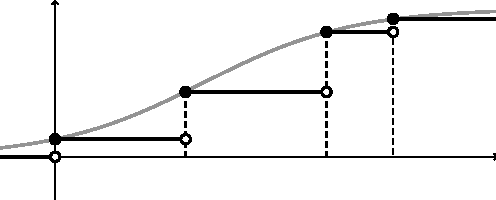
\includegraphics[width=6cm]{Images/mira}};
		\draw [color=black](-2.3,-0.75) node[anchor=north west] {$x_1$};
		\draw [color=black](-1,-0.75) node[anchor=north west] {$x_2$};
		\draw [color=black](0.7,-0.75) node[anchor=north west] {$x_3$};
		\draw [color=black](1.5,-0.75) node[anchor=north west] {$x_4$};
		\draw [color=black](-3.1,-0.85) node[anchor=north west] {$...$};
		\draw [color=black](2.2,-0.85) node[anchor=north west] {$...$};
		\end{tikzpicture}
	\end{center}
\end{define}

\begin{theorem}[ZVMS]
	Mějme $X_1,...,X_n~iid~\FF$. Pak pro~$\forall t\in\R$ fixní platí, že $\FF_n(t)$ je nestranným, konzistentním a~$\AN$ odhadem $\t=F(t)$, tzn.\begin{enumerate}
		\item $\E \FF_n(t)=\FF(t),~\forall n$,
		\item $\FF_n(t)\PSJ \FF(t),~\forall t\in\R$,
		\item $\FF_n(t)\sim\AN\left( \FF(t),\frac{1}{n}\FF(t)\br{1-\FF(t)} \right)$. 
\end{enumerate}	
	Navíc dokonce platí, že\begin{enumerate}
		\item $\sup\limits_{t\in\R}\abs{\FF_n(t)-\FF(t)}\sj 0$, (Glivenko-Cantelliho lemma),
		\item $\p{\sup\limits_{t}\abs{\FF_n(t)-\FF(t)}>\epsilon}\leq 8(n+1)\e{-\frac{n\epsilon^2}{32}},~\forall n,~\forall\epsilon>0$, (Glivenko-Cantelli),
		\item $\p{\sup\limits_{t}\abs{\FF_n(t)-\FF(t)}>\epsilon}\leq 2\e{-2n\epsilon^2},~\forall n,~\forall\epsilon>0$ (Massart, 1990).
	\end{enumerate}
	\begin{proof}
	Pro důkaz volme fixní libovolné $t$ a~označme $\Identita{(-\infty,t]}(X_j)=Y_j^t$. Pak
			 $Y_j^t=\begin{cases}
			1, & X_j\leq t, \\ 0, & \text{jinak,}
			\end{cases}$ přičemž spočteme
		$$ \PP(Y_j^t=1)=\PP(X_j\leq t)\equal{X_j~iid}P(X\leq t)=\FF(t),\quad\PP(Y_j^t=0)=1-\FF(t), $$ což nám poskytuje rozdělení $ Y_j^t\sim\A(p=\FF(t))$ - alternativní (Bernoulliho) rozdělení. $(Y_j^t)_{j=1}^n$ jsou nezávislé, protože $X_j~iid$.
		 Dále víme, že $n\FF_n(t)=\sumjn Y_j^t\sim \mathrm{Bi}\br{n,p=\FF(t)}$. Z~vlastností binomického rozdělení potom vyplývá, že 
			\begin{enumerate}[a)]
				\item $\E \FF_n(t)=\frac{1}{n}\E\big[ \mathrm{Bi}\br{n,p=\FF(t)} \big]=\FF(t)=\t,~\forall t$,
				\item $\frac{1}{n}\sumjn Y_j^t =\overbar{Y_n^t}\PSJ  \E Y_j^t=\E Y_1^t=\FF(t)=\t$\quad (ZVČ),
				\item $\FF_n(t)=\frac{1}{n}\sumjn Y_j^t =\overbar{Y_n^t}\sim\AN\Br{\FF(t),\frac{1}{n}\FF(t)\br{1-\FF(t)}}\quad\Br{\text{ CLT pro~}(Y_j^t)_{j=1}^n~iid~\LL_2\br{\mathrm{A}(p)}}$.
			\end{enumerate}
	\end{proof}
\end{theorem}

\begin{define}
	Mějme $\t=\t(\FF)$ (funkcionál na~prostoru distribučních funkcí). Pak $$T_n(\X)=\t(\underbrace{\FF_n}_{\to \FF})$$ se~nazývá \textbf{statistický funkcionál}.
\end{define}
\begin{example}
	\[
	\begin{split}
	\t(\FF)=\E X\quad &\Rightarrow\quad T_n(\X)=\t(\FF_n)=\int x\d\FF_n=\sumjn x_j\cdot\PP_n(X=x_j)=\sumjn x_j\cdot \frac{1}{n}=\Oxn, \\
	\t(\FF)=\D X\quad &\Rightarrow\quad  T_n(\X)=\t(\FF_n)=\int x^2\d\FF_n-\left( \int x\d\FF_n \right)^2=\frac{1}{n}\sumjn x_j^2-\Oxn^2=\hsn, \\
	\t(\FF)=x_{\alpha} \quad&\Rightarrow\quad T_n(\X)=\t(\FF_n)=\inf\{ x:\FF_n(x)\geq\alpha \}=\widehat{x}_\alpha,\text{ kde $x_\alpha$ je $\alpha$-kvantil $X$}.
	\end{split}
	\]
\end{example}
\begin{define}[Histogram]
	Mějme $X\sim f,~\supp f=[a,b]$, resp. zde BÚNO $[0,1]$. Zavedeme dělení intervalu $[0,1]$
	$$ B_1=\Big[0,\frac{1}{m}\Big),~B_2=\Big[\frac{1}{m},\frac{2}{m}\Big),...,~B_m=\Big[\frac{m-1}{m},1\Big] $$
	 a~označíme dále $h=\frac{1}{m}=\lambda(B_j)$, $Y_j=\#\{ i: X_i\in B_j \}_{i=1}^n$, $\widehat{p_j}=\frac{Y_j}{n}$ jako odhad $p_j=\int\limits_{B_j}f(x)\d x$. Pak \textbf{histogramový odhad hustoty pravděpodobnosti} definujeme vztahem
	$$ \widehat{f}_n^\txt{~H}(t)=\sm{j=1}{m}\frac{\widehat{p_j}}{h}\Identita{B_j}(t)=\frac{1}{nh}\sm{j=1}{m}Y_j\Identita{B_j}(t)=\frac{1}{nh}\sm{i=1}{n}\mathcal{I}{\{X_i\in B_j\}},\quad\forall t\in B_j. $$
\end{define}
\begin{theorem}[IMSE]
	Pro $\widehat{f}_n^\txt{~H}(t)$ předpokládejme, že $f'$ je absolutně spojitá a~platí, že\\ $\int\limits_{\R}\br{f'(u)}^2\d u<+\infty$. Potom
	$$ R(\widehat{f}_n^\txt{~H},f)=\frac{h^2}{12}\int\limits_{0}^1\br{f'(x)}^2\d x+\frac{1}{nh}+o(h^2)+o\Br{\frac{1}{n}}, $$
	což při~volbě $h_n=O\br{n^{-1/3}}$ vede na~řád integrované střední kvadratické chyby (\textit{Integrated Mean Square Error})
	$$ \txt{IMSE}=R(\widehat{f}_n^\txt{~H},f)=\int\limits_{0}^1\EE{\widehat{f}_n^\txt{~H}(t)-f(t)}^2\d t=O\br{n^{-2/3}}. $$
\end{theorem}
\begin{define}
	Mějme jádro $K(x)$ takové, že $K(x)\geq0,~\int\limits_{\R}K(x)\d x=1,~\int\limits_{\R}xK(x)\d x=0,~\sigma_K^2=\int\limits_{\R}x^2K(x)\d x>0$. Označíme $h\in\R^+$ jako tzv. \textbf{šířku okna} (\textit{bin width}), neboli vyhlazovací parametr (\textit{smoothing parameter}). Pak definujeme \textbf{jádrový odhad hustoty} vztahem
	$$ \widehat{f}_n^\txt{~K}(t):=\frac{1}{n}\sm{i=1}{n}\frac{1}{h}K\Br{\frac{t-X_i}{h}},\quad\forall t\in\R. $$
\end{define}
\begin{remark}
	Příklady takových používaných jader mohou být: \begin{enumerate}
		\item $K(x)=\frac{1}{2}\Identita{[-1,1]}(x)$ (boxcar),
		\item $K(x)=\frac{1}{\sqrt{2\pi}}\e{-\frac{x^2}{2}}$ (Gaussovo),
		\item $K(x)=\frac{3}{4}(1-x^2)\Identita{[-1,1]}(x)$ (Epanechnikovo) apod.
	\end{enumerate}
\end{remark}
\begin{remark}
Podobný výsledek řádu IMSE lze ukázat pro~jádrový odhad $\widehat{f}_n^\txt{~K}(t)$. Při~volbě $h_n=O\br{n^{-1/5}}$ lze dosáhnout pro~$\widehat{f}_n^\txt{~K}(t)$ řád IMSE$=O\br{n^{-4/5}}$.
\end{remark}

\chapter{Metody pro~hledání bodových odhadů}\label{kapitola2}


\section{Metoda momentů}
Tato metoda je založená na~užití výběrových momentů, ať už centrálních nebo necentrálních, případně i~z~momentů rozdělení. V~praxi pak využijeme tu, která se~dá vypočítat nejjednodušeji.
V této metodě bereme v~potaz všechny realizace.

Máme tedy $\prostor,~\t\in\Theta\subset\R^k,~\tau(\t)$ jako odhadovanou parametrickou funkci, vlastnost $X~iid~f_X(x,\t)$. Nechť $X_1,...,X_n~iid~\LL_k$ (aby existovaly momenty do~řádu $k$) a~označíme \[
\begin{split}
\mu_r&=\mu_r(\t)=\E X^r,~r\in\hat{k},\\
\bmu(\t)&=\br{\mu_1(\t),...,\mu_k(\t)}:\R^k\to\R^k.
\end{split}
\]
Dále požadujeme, aby $\exists\bmu^{-1}$, tedy například aby $\bmu$ bylo regulární a~prosté. 

\begin{define}[Momentový odhad]
	\textbf{Momentový odhah} $\t$ definujeme vztahem
	$$ \htm:=\htm(\X)=\bmu^{-1}\br{m'_1(\X),...,m'_k(\X)}\text{,\quad  kde }m'_r(\X)=\frac{1}{n}\sumjn X_j^r, $$ což znamená, že $\htm$ je řešením \textit{soustavy momentových rovnic} (značíme $ME_q$) ve~tvaru $$\mu_r(\t)=m'_r(\X),\quad \forall r \in\hat{k}.$$ Definujeme dále \textbf{momentový odhad} $\tau(\t)$ vztahem $T_\txt{M}(\X):=\tau\br{\htm(\X)}$, metoda momentů je tedy invariantní na~transformace parametru $\t$ (je to jen jiné vyjádření pro~vztah\\ $T_\txt{M}(\X)=\widehat{\tau(\t)_\txt{M}}=\tau(\htm)$).
\end{define}
\begin{remark}
	\begin{enumerate}
		\item Pokud soustava $ME_q$ není jednoznačně řešitelná, případně některý z~momentů $\mu_r$ nezávisí na~$\t$, pak můžeme přidat další rovnici ve~tvaru $\mu_{k+1}(\t)=m_{k+1}(\X)$.
		\item Alternativně lze užít i~centrální momenty
		$$ \mu_r(\t)=\E(X-\E X)^r,\qquad m_r(\X)=\frac{1}{n}\sumjn (X_j-\Oxn)^r. $$
	\end{enumerate}
\end{remark}
\begin{example}
	Mějme $\poslkon~iid~\NN(\mu,\sigma^2)$. Pak je soustava $ME_q$ ve~tvaru \[
	\begin{split}
	\E X&=\mu\stackrel{!}{=}\Oxn, \\ \E(X-\E X)^2&=\D X=\sigma^2\stackrel{!}{=}\frac{1}{n}\sumjn (X_j-\Oxn)^2=\hsn.
	\end{split}
	\] Momentové odhady $\widehat{\mu}_\txt{M} = \Oxn$ a~$\widehat{\sigma}^2_\txt{M}=\hsn$ jsou tedy konzistentní a~$\AN$ odhady $\mu$ a~$\sigma^2$. Obecně však momentové odhady nejsou eficientní.
\end{example}
\begin{theorem}
	Pokud je $\inv{\bmu}$ spojitá funkce, pak $\htm(\X)$ je \textbf{konzistentním} odhadem $\t$. Pokud je navíc $\tau$ spojitá, pak $T_\txt{M}(\X)$ je konzistentní.
	\begin{proof}Ze ZVČ (Chinchin) víme, že 
		$m_1(\X)\PSJ\mu_1,...,m_k(\X)\PSJ\mu_k$. Pak ale
		$$
		\htm=\inv{\bmu}\br{m_1(\X),...,m_k(\X)}\PSJ\inv{\bmu}(\mu_1,...,\mu_k)=\inv{\bmu}(\bmu(\t))=\t.$$
		Podobně pak $T_\txt{M}(\X)=\tau(\htm)\PSJ\tau(\t)$ pro~$\tau(\t)$ spojité.
	\end{proof}
\end{theorem}

\begin{remark}[Připomínka Delta metody] Mějme $\poslnn$ do~$\R^k,~\X_n\sim\AN_k\br{\theta,\frac{1}{n}\C(\theta)}$. Nechť $g:\R^k\to\R$ je borelovská, $\nabla g(\theta)\neq 0,~\exists\frac{\partial g}{\partial\theta_i}$ na~$H_\theta$ (okolí $\theta$) a~jsou spojité v~bodě $\t$. Pak $$ g(\X_n)\sim\AN_1\Br{g(\theta),\frac{1}{n}\nabla g(\theta)\C(\theta)\nabla g(\theta)^T}. $$
	Zobecnění pro~$g:\R^k\to\R^k$: Pokud Jacobiho matice $\mathbb{J}_g$ zobrazení $g$ existuje na~okolí $H_\t$ a~je spojitá v~bodě $\t$, $\mathbb{J}_g(\t)\neq \textbf{0}$, pak
	$$ g(\X_n)\sim\AN_k\Br{g(\t),\frac{1}{n}\mathbb{J}_g(\t)\C(\t)\mathbb{J}_g(\t)^T}. $$
\end{remark}

\begin{theorem}
	Nechť $\htm$ je odhad metodou momentů, $\posl\in\LL_{2k},~\bmu$ je difeomorfismus $(\bmu,\inv{\bmu}$ spojitě diferencovatelné$)$. Pak $\forall\t\in\Theta$ je $$\htm\sim\AN\Br{\t,\frac{1}{n}\C_\txt{M}(\t)},$$ kde $\C_\txt{M}(\t)=\mathbb{J}_{\inv{\mu}}(\t)\C(\t)\mathbb{J}_{\inv{\mu}}(\t)^T$ a~$\C=\Cov(X,X^2,...,X^k)$.  Pokud je navíc $\tau(\t)$ spojitě diferencovatelné a~$\nabla\tau(\t)\neq0$, pak $$T_\txt{M}(\X)\sim\AN\br{\tau(\t),\frac{1}{n}\nabla\tau(\t)\C_\txt{M}(\t)\nabla\tau(\t)^T}.$$
	\begin{proof}
		Definujeme $\mathbb{Z}_j:=(X_j,X_j^2,...,X_j^k)$. Potom
		$$ \E \mathbb{Z}_j=(\E X_j,\E X_j^2,...,\E X_j^k)=(\E X,\E X^2,...,\E X^k)=\bmu(\t). $$
		Označme nyní $\Cov (\mathbb{Z}_j)=\Cov(X,X^2,...,X^k)=\C(\t)$. Víme, že $\mathbb{Z}_j~iid~\LL_2$, tudíž dle CLT v~$\R^k$ platí, že $\overline{\mkern-1mu \mathbb{Z}_n \mkern-3mu}=\br{m_r(\X)}_{r=1}^k\sim\AN_k\br{\bmu(\t),\frac{1}{n}\C(\t)}$. Pak pro~$g=\inv{\bmu}$ spojitě diferencovatelné dostáváme z~$\Delta$-metody vztah
		$$ \htm=\inv{\bmu}\Br{\br{m_r(\X)}_{r=1}^k}\stackrel{\ref{lamatko}}{\sim}\AN\Br{\t,\frac{1}{n}\underbrace{\mathbb{J}_{\inv{\mu}}(\t)\C(\t)\mathbb{J}_{\inv{\mu}}(\t)^T}_{\C_\txt{M}(\t)}}. $$
		Následně pro~$\tau$ spojitě diferencovatelné opět z~$\Delta$-metody dostaneme, že
		$$ T_\txt{M}(\X)=\tau(\htm)\sim\AN\Br{\tau(\t),\frac{1}{n}\nabla\tau(\t)\C_\txt{M}(\t)\nabla\tau(\t)^T}. $$
	\end{proof}
\end{theorem}
\begin{example}
	Mějme $X_1,...,X_n~iid~\n{\mu,\sigma^2}$, kde neznáme hodnotu parametrů $\mu$ a~$\sigma^2$. Víme ale, že 
	$$ \E X_i=\mu,\quad \D X_i=\sigma^2\text{\quad a\quad }\E (X_i)^2=\D X_i+(\E X_i)^2=\sigma^2+\mu^2. $$
	Odhady parametrů metodou momentů dostaneme z~rovnic
	$$ \mu=m_1'=\Oxn\text{\quad a\quad }\sigma^2=m_2 =\frac{1}{n}\br{\sumjn X_j-\Oxn}^2=\hsn. $$
	Tím získáme odhady $\widehat{\mu}_\txt{M},~\widehat{\sigma}_\txt{M}^2$.
\end{example}
\section{Nestranné odhady s~minimálním rozptylem (UMVUE)}

\begin{define}
	Mějme $X_1,...,X_n~iid~\FF,~\t\in\Theta\subset\R^k,~\tau(\t)\in\R^1,~T(\X)$ jako odhad $\tau(\t)$. Definujeme $$T_{\txt{UMR}}=\argmin\limits_T \E\br{T(\X)-\tau(\t)}^2,\quad\forall\t\in\Theta.$$
	Definujeme dále kvadratickou \textbf{ztrátovou funkci} (\textit{loss function}) jako $$\Loss_2(T,\t):=\br{T(\X)-\tau(\t)}^2$$
	a příslušnou \textbf{rizikovou funkci} (\textit{risk function}) vztahem $$R(T,\t):=\E \Loss_2(T,\t).$$ Potom $T_{\txt{UMR}}=\argmin\limits_TR(T,\t)$, kde
	UMR je zkratka pro~\textit{uniformly minimum risk}. $T_{\txt{UMR}}$ je tedy odhad, který minimalizuje hodnotu rizikové funkce $R$.
\end{define}
\begin{define}
	$S(\X)$ se~nazývá \textbf{postačující statistika} (\textit{sufficiency}) pro~$\t$, pokud rozdělení $\X$ podmíněné hodnotou $S(\X)=s$ nezávisí na~parametru $\t$. Pro~diskrétní případy tedy\newline $\PP(\X=\textbf{x}|S(\X)=s)$ nezávisí na~$\t$, případně $f_{\X | S}(\textbf{x}|s)$ nezávisí na~$\t$.
	\\ \\
	Postačující statistika je tedy taková funkce náhodného výběru (statistika), která umí sama o~sobě nahradit původní výběr bez~ztráty informace o~parametru $\t$.
\end{define}
\begin{example}
	Házíme mincí, $X_i\sim\Be(\t)$, $\textbf{x}=(0,1,1,0,1,...)$. Představme si, že chceme vypočítat tzv. MLE (bude definováno později) ve~tvaru $$ L=\prod\limits_{i=1}^N \t^{x_i}(1-\t)^{1-x_i}\qquad=\t^{x_1+x_2+...}(1-\t)^{1-x_1+1-x_2+...}=\t^{\sm{i=1}{N}x_i}(1-\t)^{N-\sm{i=1}{N}x_i}. $$
	Pak ale ve~výsledku nezáleží na~samotných datech, ale pouze na~jejich součtu, tedy pokud označíme $S(\X):=\sm{i=1}{N}X_i$, pak $S(\X)$ je postačující statistika (podle Neymannova fatrorizačního kritéria).
	%https://www.youtube.com/watch?v=5j4E2FRR384
\end{example}
\begin{define}	Mějme $X,Y$ náhodné veličiny na~$\prostor$. Pak $$\E(X|Y=y)=\int\limits_{\R} x\d \PP^{X|Y=y}=\Big[\text{pro ASR }f_{X|Y}(x|y):=\frac{f_{X,Y}(x,y)}{f_Y(y)}\Big]=...$$
	Z toho vyplývá, že $\E(X|Y):\Omega\to\R$ je náhodná veličina.
\end{define}

\begin{theorem}
	Pro náhodné veličiny $(X,Y)$ s~ASR $f_{X,Y}$ platí vztah
	$$ \E\big[\E(X|Y)\big]\equal{\text{ASR}}\int\limits_{\R} \Br{\int\limits_{\R} xf_{X|Y} \d x} f_Y\d y \equal{\text{F.V.}}\int\limits_{\R}\Br{\int\limits_{\R} f_{X|Y}f_Y\d y}x\d x=\int\limits_{\R}\Br{\int\limits_{\R} f_{X,Y}\d y}x\d x=\int\limits_{\R} xf_X\d x=\E X. $$	
\end{theorem}
 ~\\
Pro účely následující Rao-Blackwellovy věty označme $$T_{\txt{RB}}(\X)=T_{\txt{RB}}\br{S(\X)}:=\E\big[ T(\X)|S(\X)=s \big]$$ za~předpokladu existence $\E$ jako odhad zkonstruovaný v~Rao-Blackwellově větě. 
$T_{\txt{RB}}(\X)$ je tedy opět statistika, pro~kterou platí, že $$ T_{\txt{RB}}(\X):=\E\big[ T(\X)|S(\X)=s \big]\equal{\text{ASR}}\int T(\textbf{x})f_{T(\X)|S(\X)=s} \d \textbf{x}.$$
Na $T_\txt{RB}(\X)$ pohlížíme jako na~funkci $\X$, která vznikne ve~dvou krocích:\begin{enumerate}
		\item spočítá se~podmíněná střední hodnota $\E\br{T(\X)|S(\X)=s}=T(s)$ při~libovolně daném pevném $s$,
		\item za~$s$ se~dosadí vazba $s=S(\X)$, čímž vznikne $T_\txt{RB}\br{S(\X)}$.
	\end{enumerate}


\begin{theorem}[Rao-Blackwell]
		Mějme $X_1,...,X_n~iid~\FF,~\t\in\Theta\subset\R^k,~\tau(\t)\in\R^1,~T(\X)$ jako odhad $\tau(\t)$, nechť $S(\X)$ je postačující statistika pro~$\t$ a~nechť $\Loss(T,\t)$ je konvexní funkcí v~$T$ pro~$\forall\t\in\Theta$.
	Pak $$R\br{T_{\txt{RB}}(\X),\t}\leq R\br{T(\X),\t},\quad\forall\t\in\Theta,$$ přičemž $T_{\txt{RB}}$ nezávisí na~$\t$. 
\begin{proof}Větu ukážeme obecněji pro~$\Loss(T,\t)$ konvexní v~$T$, která zahrnuje i~naši kvadratickou ztrátovou funkci $\Loss_2$. Pro~$\forall\t\in\Theta$ z~Jensenovy nerovnosti platí, že
	$$R(T_{\txt{RB}},\t)=\E \Loss\br{\EE{T| S=s},\t}\leq\E\big[ \EE{\Loss(T,\t)|S=s} \big]=\E \Loss(T,\t)=R(T,\t).$$
\end{proof}
\end{theorem}
\begin{define}
	Systém hustot $\mathcal{F}=\mathcal{F}_X=\{ f(x,\t):\t\in\Theta\subset\R^k \}$ se~nazývá \textbf{úplný}, pokud pro~
	$\forall h:\R\to\R,~\E_\t h(X)=0,~\forall\t\in\Theta$ platí, že$$ h(X)=0~s.j.\quad \forall\t\in\Theta,\quad \text{neboli}\quad \PP_\t\br{h(X)=0}=1.$$
\end{define}
\begin{define}
	Postačující statistika $S$ se~nazývá \textbf{úplná postačující statistika}, pokud systém rozdělení $\mathcal{F}_S$ je úplný, tzn. pro~libovolnou borelovskou funkci $g:\R\to\R$ platí, že pokud
	$$ \EE{g(S(X))}=0,~\forall\t\in\Theta,\quad\text{pak}\quad g\br{S(X)}=0~s.j.,~\forall\t\in\Theta. $$
\end{define}
\begin{theorem}[Lehmann-Scheffé]
	Nechť jsou splněny předpoklady R.-B. věty a~navíc $T(\X)$ je nestranný odhad $\tau(\t)~($tzn. $\E T=\tau,~\forall\t\in\Theta)$, a~dále nechť $S(\X)$ je úplná postačující statistika. Pak $T_{\txt{RB}}=T_\txt{UMR}$, což pro~volbu ztrátové funkce $\Loss_2$ označíme jako $T_\txt{UMVUE}$. (\textit{uniformly minimum variance unbiased estimator})
	\begin{proof}
		\begin{itemize}
			\item 	Z předpokladu víme, že $T$ je nestranné, tedy i~$T_{\txt{RB}}$ je nestranné, protože\newline $\E T_{\txt{RB}}=\E\big[ \E(T|S=s) \big]=\E T=\tau(\t),~\forall\t\in\Theta$.
			\item $T_{\txt{RB}}$ nestranné $\Rightarrow R(T_{\txt{RB}},\t)=\E \Loss_2(T_{\txt{RB}},\t)=\E\br{T_{\txt{RB}}(\X)-\underbrace{\tau(\t)}_{\E T_\txt{RB}(\X)}}^2=\D \big[T_{\txt{RB}}(\X)\big]$.
			\item $T_{\txt{RB}}=T_\txt{UMVUE}:~T^{(1)},T^{(2)}$ oba nestranné odhady $\tau(\t)$. Z~toho vyplývá, že 
			$ T_{\txt{RB}}^{(1)}$ a~$T_{\txt{RB}}^{(2)}$ jsou také nestranné odhady $\tau(\t)$. Potom ale $$\E\Br{T_{\txt{RB}}^{(1)}-T_{\txt{RB}}^{(2)}}=0~\stackrel{\text{S je úplná}}{\Longrightarrow}~T_{\txt{RB}}^{(1)}-T_{\txt{RB}}^{(2)}=0\quad s.j.~\forall\t\in\Theta, $$
			protože na~$T_{\txt{RB}}^{(1)}-T_{\txt{RB}}^{(2)}$ aplikujeme úplnou postačující statistiku $S(\X)=s$.
		\end{itemize}
	\end{proof}
\end{theorem}
\begin{remark}
	$T_\txt{RB}$ jen stejnoměrně vylepšuje, ale nemusí dosahovat na~ten stejnoměrně nejlepší. Že z~R-B věty vyleze ten úplně nejlepší, který už nelze stejnoměrně vylepšit, právě zajišťují předpoklady Lehmann-Scheffé.
	
		Pozor, UMVUE není invariantní na~transformace, tzn. $\widehat{\tau(\t)}_\txt{UMVUE}\neq\tau(\hat{\t}_\txt{UMVUE})$.
\end{remark}
\section{Rao-Cramérova nerovnost}
\begin{define}\label{reghustoty}
	Mějme $\mathcal{F}=\{ f(x,\t):~\t\in\Theta\subset\R^k \}$ a~označíme $$l(\t)=\ln f(x,\t),\quad l'_i(\t):=\frac{\partial}{\partial \t_i}\ln f(x,\t),\quad \nabla_\t l=\nabla l(\t)=\br{l'_1(\t),...,l'_k(\t)}.$$
	Systém $\mathcal{F}$ se~nazývá \textbf{regulární systém hustot}, ozn. $\freg$, pokud\begin{enumerate}[\quad1)]
			\item $\supp f$ nezávisí na~$\t$ a~$\Theta$ je otevřená množina,
			\item pro~všechna $\forall\t\in\Theta$ existuje $\nabla l(\t)$ na~$\supp f$,
			\item $\E\big[\nabla l(\t)\big]=0,~ \forall\t\in\Theta,$ což je zajišěno předpokladem následující záměny$$\E\big[l'_i(\t)\big]=\int\limits_{\R}\frac{f_i'}{f}\cdot f\d x=\int\limits_{\R}\frac{\partial}{\partial\t_i}f\d x=\frac{\partial}{\partial\t_i}\underbrace{\int\limits_{\supp f} f\d x}_{=1}=0,$$
			\item $\Cov\br{\nabla l(\t)}$ je konečná a~PD matice rozměru ($k\times k$).
		\end{enumerate}
		Systém $\mathcal{F}$ označíme $\fregp$, pokud navíc splňuje podmínku\begin{enumerate}[\quad5)]
			\item $\E\Big[\frac{f_{i,j}''(\X,\t)}{f(\X,\t)} \Big]=0,~\forall\t\in\Theta,\quad$neboli $\int\limits_{\R^n}\frac{\partial^2}{\partial\t_i\partial\t_j}f(\textbf{x},\t)\d\textbf{x}=0,~\forall\t\in\Theta$.
		\end{enumerate}
\end{define}
\begin{define}
	$\fisher(\t)=\Cov\br{\nabla l(\t)}$ se~nazývá \textbf{Fisherova informační matice} a~platí, že 
	$$ \fisher_{i,j}(\t):=\Cov(l'_i,l'_j)=\E(l'_i\cdot l'_j)-\underbrace{\E l'_i}_{=0}\underbrace{\E l'_j}_{=0}=\E\Br{\frac{\partial\ln f}{\partial\t_i}\cdot \frac{\partial\ln f}{\partial\t_j}}\equal{5)}-\E\Big[ \frac{\partial^2 \ln f}{\partial\t_i\partial\t_j} \Big]. $$
	
\end{define}
\begin{lemma}
	Mějme $\X=(X_1,...,X_n)$ nezávislé, $X_i\sim f_{X_i}(x_i,\t)$. Pak $\fisher_\X(\t)=\sumjn \fisher_{X_j}(\t)$. Pokud navíc $X_1,...,X_n$ jsou $iid~f_X$, pak  $\fisher_\X(\t)=n\fisher_X(\t)$.
	\begin{proof}Speciálně pro~systém $\fregp$ dostaneme
	$$ (\fisher_\X)_{ij}(\t)=-\E\Big[ \frac{\partial^2 \ln f}{\partial\t_i\partial\t_j} \Big] =-\E\Bigg[ \frac{\partial^2 \ln \prod\limits_{l=1}^n f_{X_l}}{\partial\t_i\partial\t_j} \Bigg]=-\sum\limits_{l=1}^n\EE{\frac{\partial^2\ln f_{X_l}}{\partial\t_i\partial\t_j}}=\sum\limits_{l=1}^n(\fisher_X)_{ij}(\t).  $$
	\end{proof}
\end{lemma}
\begin{theorem}[Rao-Cramérova nerovnost]
	Mějme $T(\X)$ jako nestranný odhad $\tau(\t)$, $\freg$, nechť dále $(\forall\t\in\Theta)\br{\exists\nabla\tau(\t)}$ a~$\E\big[T(\X)\big]$ lze derivovat podle $\t_i$ pod~znakem $\E$ (tj. derivace pod~integrálem) pro~$\forall i\in\hat{k}$. Pak $$ \D\br{T(\X)}\geq \underbrace{\nabla\tau(\t)\fisher_\X^{-1}(\t)\nabla\tau(\t)^T}_{\mathrm{RCLB}_\tau(\t)},\quad \forall\t\in\Theta.\quad \br{\txt{RCLB}\text{ = Rao-Cramérova spodní hranice}}. $$
	\begin{proof}[Náznak důkazu]Označme $ \mathbb{D}:=\left(\begin{array}{cc}
		\D T(\X) & \nabla\tau \\ 
		\nabla\tau^T & \fisher_\X(\t)
		\end{array} \right)$.
	Protože každá kovarianční matice je PSD, stačí dokázat, že se~jedná o~$\Cov$ matici vektoru $(T,l'_1,...,l'_k)$, tedy že $\mathbb{D}=\Cov(T,l'_1,...,l'_k)$. To plyne z~následujícího výpočtu:
	$$\frac{\partial\tau}{\partial\t_i}(\t)=\frac{\partial}{\partial\t_i}\int T(\X)f_\X(\textbf{x},\t)\d \textbf{x}=\int T\frac{f'_i}{f}f\d \textbf{x}=\int T\frac{\partial\ln f}{\partial\t_i}f\d \textbf{x}= \E\Br{T\frac{\partial\ln f}{\partial\t_i}}=\Cov(T,l'_i),$$
	protože střední hodnota $\E l'_i$ je nulová, což víme z~regularity systému $\mathcal{F}$. Pak tedy
	$|\mathbb{D}|\geq0$ a	
	R.-C. nerovnost získáme z~rozvoje $\abs{\mathbb{D}}$ podle 1. řádku a~poté podle 1. sloupce. Tím se~získá dvojná suma, ze~které se~vyjádří $\D T(\X)$. Následně se~použije Cramerovo pravidlo pro~$\fisher_{ij}^{-1}(\t)$.
	\end{proof}
\end{theorem}
\begin{define}
	Mějme $\freg$. Pak definujeme \textbf{eficienci} nestranného odhadu $T_n(\X)$ funkce $\tau(\t)$ vztahem 
	$$ e_n:=\frac{\mathrm{RCLB}_\tau(\t)}{\D\br{T_n(\X)}}. $$ Pokud $e_n=1,~\forall n\in\N$, případně $\lim\limits_{n\to+\infty}e_n=1$, pak $T(\X)$ nazýváme \textbf{(asymptoticky) eficientní}.
	\\ \\
	Speciálně volme do definice \ref{reghustoty} jednorozměrný $\t\in\Theta\subset\R^1$. Pak $\fregp$ je definován následnovně: \[
	\begin{split}
 &1),2),3)~\E\Big[\frac{\partial\ln f}{\partial\t}(x,\t)\Big]=0, \\
	&4)~\fisher(\t)=\D\Br{\frac{\partial\ln f}{\partial\t}}\equal{5)}-\E\Big[\frac{\partial^2\ln f}{\partial\t^2}\Big]\text{, což se~nazývá \textbf{Fisherova informace} o~}\t.
	\end{split}
	\]
	Pak R.-C.N. přechází do~tvaru $\D\br{T(\X)}\geq \frac{[\tau'(\t)]^2}{\fisher_\X(\t)},~\forall\t\in\Theta$, přičemž  rovnost nastane právě tehdy, když $|\mathbb{D}|=\begin{array}{|cc|}
	\D T & \tau' \\ 
	\tau' & \fisher_\X(\t)
	\end{array}=0 $. Z~toho vyplývá, že  
	$$\D T\cdot\fisher_\X(\t)=
	\tau'(\t)^2=
	\Cov^2\Br{T,\frac{\partial\ln f}{\partial\t}}=
	\D T\cdot\D\Br{\frac{\partial\ln f}{\partial\t}}.$$ 
	Po odmocnění pak dostaneme rovnost ve~Schwarzově nerovnosti, která nástává právě tehdy, když veličiny $(T-\tau)$ a~$\frac{\partial\ln f}{\partial\t}$ jsou lineárně závislé s.j., tzn.
	\begin{equation}\label{rovnicka}
	\frac{\partial\ln f_\X}{\partial\t}=\sumjn\frac{\partial\ln f_{X_j}}{\partial\t}=K(\t,n)\br{T(\X)-\tau(\t)},\quad s.j.
	\end{equation} 
\end{define}
\begin{example}
	Nechť $f_\X(\textbf{x},\t)=c(\t)h(\textbf{x})\e{Q(\t)T(\textbf{x})}$, tzn. $\mathcal{F}$ je exponenciální třída hustot. Pak \[
	\begin{split}
	\ln f_\X(\textbf{x},\t)&=\ln c(\t)+\ln h(\textbf{x}) +Q(\t)T(\textbf{x})\text{ a~dále} \\
	\frac{\partial\ln f_\textbf{x}}{\partial\t}&=\frac{c'(\t)}{c(\t)}+Q'(\t)T(\textbf{x})=Q'(\t)\Big[ T(\textbf{x})-\underbrace{\Br{-\frac{1}{c(\t)}\cdot \frac{c'(\t)}{Q'(\t)}}}_{\tau(\t)} \Big].
	\end{split}
	\]
	Tedy pokud $T(\X)$ je nestranný a~$\tau(\t)=-\frac{1}{c(\t)}\frac{c'(\t)}{Q'(\t)}$ (předpokládáme existenci $c'(\t)$ a~$Q'(\t)$), pak z~rovnice (\ref{rovnicka}) získáváme $\txt{UMVUE}~T(\X)$ pro~$\tau(\t)$.
\end{example}
\begin{theorem}[Bhattacharya]
	Mějme $\t\in\Theta\subset\R^1$, $T(\X)$ jako odhad $\tau(\t)$. Nechť dále existuje vektor derivací podle $\t$ do~řádu $m$:~ $\tilde{\tau}'=\br{\tau',\tau'',...,\tau^{(m)}}$. Pak za~podobných dodatečných předpokladů jako v~R.-C.N., platí, že$$\D\br{T(\X)}\geq \tilde{\tau}'(\t)\tilde{\fisher}_\X^{-1}(\t)\br{\tilde{\tau}'(\t)}^T,\quad (\text{Bhattacharyova spodní hranice},~\txt{BLB}_\tau(\t)),$$ kde $\tilde{\fisher}_\X=\Cov\Br{\br{\frac{\partial^i f}{\partial\t^i}/f}_{i=1}^m}$.
\end{theorem}
\begin{remark}
	Pro $m=1$ přechází $\txt{BLB_\tau(\t)}$ na~$\txt{RCLB}_\tau(\t)$. 
	Pokud se~ani pomocí této $\txt{BLB}$ nedosáhne hranice, je třeba hledat $\txt{UMVUE}$ prostřednictvím R-B věty: $T_\txt{UMVE}=\E[T|S=s]$.
\end{remark}

\section{Metoda maximální věrohodnosti (MLE)}
MLE je ve~statistice velice často používaná metoda, pomocí které hledáme bodové odhady parametrů.  Snažíme se~maximalizovat sdruženou hustotu experimentu vzhledem k~parametru, který je obsažen v~navrženém rozdělení. Předpokládáme totiž, že známe toto rozdělení, jen neznáme jeho parametr. Tímto způsobem získáme tzv. \textbf{věrohodnostní funkci}.
\begin{define}[Věrohodnostní funkce]
 Mějme $X_1,...,X_n$ s~odpovídajícím systémem hustot $\mathcal{F}=\{ f_\X(\textbf{x},\t):\init{k} \}$. Pak definujeme \textbf{věrohodnostní funkci} vztahem $$L(\t)=f(\textbf{x},\t),\quad\text{resp.}\quad L(\t,\textbf{x})=h(\textbf{x})f(\textbf{x},\t),\quad\forall\t\in\Theta,~\forall\textbf{x}\in\R^n$$ a~\textbf{logaritmickou věrohodnostní funkci} vztahem $$l(\t)=\ln L(\t,\textbf{x}).$$
	Mějme nezávislý náhodný výběr $X_1,...,X_n~id$. Pak věrohodnostní funkci můžeme zavést jako sdruženou hustotu tohoto výběru při~dané realizaci $\textbf{x}=(x_1,...,x_n)$, tedy
	$$ L(\theta)=\prod\limits_{i=1}^{n}f_{X_i}(x_i,\theta),\quad \left( L(\theta)=\prod\limits_{i=1}^n \PP_\theta(X_i=x_i) \text{ - pro~diskrétní případ}\right).$$
\end{define}
\begin{define}[Maximálně věrohodný odhad]
 Definujeme \textbf{maximálně věrohodný odhad} vztahem $$\html(\X)=\argsup\limits_{\ini}L(\t)$$ za~předpokladu, že $\html$ je borelovsky měřitelná, jednoznačná a~závisí na~$\X$. Dále pak definujeme  \textbf{maximálně věrohodný odhad} parametrické funkce $\tau(\t)$ jako
 $$T_\txt{ML}(\X)=\tau(\html),\quad\text{tedy MLE je invariantní na~transformace }\tau.$$
\end{define}
\begin{remark}
Postup v~praxi:\\maximalizujeme $L(\theta_1,..,\theta_k)$ přes všechny možné hodnoty $\theta_1,...,\theta_k$. Vzhledem ke~tvaru $L$ je ale vhodné ji nejprve zlogaritmovat (logaritmus je monotonní a~nemění proto polohu maxima). To je právě důvod, proč se~zavádí $l(\t_1,...,\t_k)=\ln L(\t_1,...,\t_k)$. Potom získáme
$$ \frac{\partial\ln L(\theta_1,...,\theta_k)}{\partial \theta_i}=\frac{\partial l(\theta_1,...,\theta_k)}{\partial \theta_i}=0,~i\in\hat{k}, $$ který nazveme \textbf{systém věrohodnostních rovnic}, ozn $LE_q$.
\end{remark}
\begin{theorem}\label{vetaspravdepodobnosti}
	Mějme $\posl~iid~f(x,\t_0),$ kde $\supp f_\X$ nezávisí na~$\t,~\ln\frac{f(X,\t)}{f(X,\t_0)}\in\LL_1$. Dále předpokládáme identifikovatelnost rodiny hustot, tzn. $$\t_1\neq\t_2\Rightarrow \PP_{\t_1}\neq \PP_{\t_2}\text{ (různé parametry definují různá rozdělení).}$$ Pak $\PP_{\t_0}\br{L(\t_0,\textbf{x})>L(\t,\textbf{x})}\stackrel{n\to+\infty}{\longrightarrow}1,~\forall\t\neq\t_0$.
	\begin{proof}

		$$ \PP_{\t_0}\Br{\frac{L(\t,\textbf{x})}{L(\t_0,\textbf{x})}<1}=\PP_{\t_0}\Br{\frac{1}{n}\ln\frac{L(\t,\textbf{x})}{L(\t_0,\textbf{x})}<0}\equal{iid}\PP_{\t_0}\Br{\underbrace{\frac{1}{n}\sumjn\ln\frac{f(x_j,\t)}{f(x_j,\t_0)}}_{\Pto a<0}<0} $$
		Podle ZVČ aplikovaného na~$Y_j=\ln\frac{f(X_j,\t)}{f(X_j,\t_0)}$ dostaneme $\frac{1}{n}\sumjn Y_j\stackrel{\PP_{\t_0}}{\to}\E_{\t_0} Y_1$. Podle Jensenovy nerovnosti pro~ryze konkávní transformaci $\ln(u)$ potom plyne, že 
		$$\E_{\t_0} Y_1=\E_{\t_0}\Br{\ln\frac{f(X_1,\t)}{f(X_1,\t_0)}}< \ln\E_{\t_0}\Br{\frac{f(X_1,\t)}{f(X_1,\t_0)}}=\ln\int\limits_{\R} \frac{f(x,\t)}{f(x,\t_0)}f(x,\t_0)\d x= \ln\int\limits_{\R} f(x,\t)\d x=0. $$
		Nyní využijeme implikaci (důkaz ponechán čtenáři) $\Br{Y_n\Pto a<0~\Rightarrow~\PP(Y_n<0)\to1}$, díky~kterému plyne tvrzení věty, tzn.  $\PP_{\t_0}\br{\frac{L(\t,\textbf{x})}{L(\t_0,\textbf{x})}<1}\stackrel{n\to+\infty}{\longrightarrow}1$.
	\end{proof}
\end{theorem}
\begin{define}
	Systém hustot $\mathcal{F}:=\{ f(x,\t):~\init{k} \}$ se~nazývá \textbf{ML-regulární}, ozn. $\fregml$, pokud pro~něj platí, že \begin{enumerate}
		\item $\Theta$ je otevřená množina, $\supp f_X$ nezávisí na~$\t$,
		\item $f(x,\t)\in\Cc^{(3)}$ vzhledem k~$\t$ pro~$\forall x\in\R$,
		\item $\int\limits_{\R} \frac{\partial f}{\partial\t_r}\d x=0$ \quad a\quad  $\int\limits_{\R} \frac{\partial^2 f}{\partial\t_r\partial\t_j}\d x=0,\quad \forall\t\in\Theta$, tzn. záměna derivací a~integrálu je možná,
		\item  Fisherova informační matice $\fisher_X(\t)$ je PD a~konečná,
		\item \mbox{$(\forall\t_0)(\exists H_{\t_0})\br{\exists M(X)\in\LL_1(\PP_{\t_0})}(\forall\t\in H_{\t_0})\Br{\nor{\partial_\t^3\ln f}\leq M(X),~\text{přičemž }\E_{\t_0} M(X)<+\infty}.$}
	\end{enumerate}
\end{define}
\begin{define}\label{definicka}
	Mějme $ \widehat{\t}_n\sim\AN\br{\t_0,\frac{1}{n}\C(\t)}$. $ \widehat{\t}_n$ se~nazývá  \textbf{asymptoticky eficientní}, pokud $\C(\t)=\inv{\fisher_X}(\t_0)$.
\end{define}
\begin{theorem}
	Mějme $X_1,...,X_n~iid~f(x,\t_0)\in\fregml$. Pak pro~každé konzistentní řešení $ \widehat{\t}_n(\X)$ soustavy věrohodnostních rovnic $LE_q$ platí, že  $$\widehat{\t}_n\sim\AN_k\Br{\t_0,\frac{1}{n}\inv{\fisher_X}(\t_0)}\text{,\quad  neboli \quad }\sqrt{n}\br{\widehat{\t}_n(\X)-\t_0}\Dto \NN_k\Br{0,\frac{1}{\fisher_X(\t_0)}}.$$
	Takové konzistentní řešení je tedy $\AN$ a~dle definice \ref{definicka} i~asymptoticky eficientním odhadem $\t_0$, ozn. $\widehat{\t}_\txt{ELE}$ (\textit{ELE = eficient likelihood estimator}).
	\begin{proof}[Důkaz pro~$k=1$] $\widehat{\t}_n$ je $\underbrace{\text{konzistentní řešení}}_{\widehat{\t}_n\Pto\t_0}\text{ rovnice }\frac{\partial l_n}{\partial \t}(\t,x)=0,$ tedy $l_n'(\widehat{\t}_n)=0$, kde \\$l_n(\t)=\ln \prod\limits_{i=1}^nf_{X_i}(x,\t)$. Nyní uděláme Taylorův rozvoj $l_n'(\widehat{\t}_n)$ do~2. řádu, tedy
		$$ l_n'(\widehat{\t}_n)=l_n'(\t_0)+(\widehat{\t}_n-\t_0)l_n''(\t_0)+\frac{1}{2}(\widehat{\t}_n-\t_0)^2l_n'''(\t_n^\ast)=0,\quad \text{kde }\t_n^\ast\in /\widehat{\t}_n,\t_0/. $$ 
		Z této rovnice vyjádříme $\sqrt{n}(\widehat{\t}_n-\t_0)$ v~následujícím tvaru: $$\sqrt{n}(\widehat{\t}_n-\t_0)=\frac{-\overbrace{\frac{1}{\sqrt{n}}l_n'(\t_0)}^{4)~\Dto\n{0,\fisher_X(\t)}} }{\underbrace{\frac{1}{n}l_n''(\t_0)}_{1)~\Pto  -\fisher_X(\t_0)}+\frac{1}{2}\underbrace{(\widehat{\t}_n-\t_0)}_{2)~\Pto0}\underbrace{\frac{1}{n}l_n'''(\t_n^\ast)}_{3)~\Pto C<+\infty}} \Dto \frac{1}{\fisher_X(\t)}\n{0,\fisher_X(\t)}\quad (\text{Stutskyho lemma}.) $$ Nyní rozebereme jednotlivé části vzniklého výrazu:
		\begin{enumerate}[1)]
			\item  \[\begin{split}
			\frac{1}{n}l_n''(\t_0)&=\frac{1}{n}\Br{\ln \prod\limits_{j=1}^{n}f_{X_j}}''=\frac{1}{n}\sumjn(\ln f_{X_j})''=\frac{1}{n}\sumjn l_j''(\t_0)\stackrel{\PP~(\text{ZVČ})}{\longrightarrow}\E\big[l_1''(\t_0)\big]=\\ &=\E\Big[\frac{\partial^2 \ln f_{X_1}}{\partial\t^2}\Big]=-\fisher_X(\t_0)
			\end{split}\] 
			\item $\widehat{\t}_n-\t_0 \Pto0$, protože $\widehat{\t}_n$ je konzistentním řešením $LE_q$.
			\item Zde využijeme předpoklad č. 5 z~definice, $\fregml$. $$ \Big|\frac{1}{n}l_n'''(\t_n^\ast)\Big|=\Big|\frac{1}{n}\sumjn l_j'''(\t_n^\ast)\Big|\leq \frac{1}{n}\sumjn\Big| l_j'''(\t_n^\ast)\Big|\leq\frac{1}{n}\sumjn M(X_j)\stackrel{\PP~(\text{ZVČ})}{\longrightarrow}\E M(X)=C<+\infty. $$			
			\item CLT říká, že pro~$Y_1,...,Y_n~iid$ platí, že $\sqrt{n}(\oyn-\mu)=\sqrt{n}\Br{\frac{1}{n}\sumjn Y_j-\E Y_1}\Dto\NN(0,\D Y_1)$. Zkusíme se~tedy dostat do~tohoto tvaru.
			$$ \frac{1}{\sqrt{n}}l_n'(\t_0)\equal{iid}\sqrt{n}\Br{\frac{1}{n}\sumjn l_1'(\t_0)-\underbrace{\E l_1'(\t_0)}_{=0}}\Dto \NN\Br{0,\D\br{l_1'(\t_0)}}=\NN\Br{0,\underbrace{\E\Big[\frac{\partial}{\partial\t}\ln f(X_j,\t_0)\big]}_{\fisher_X(\t_0)}}, $$
			kde člen $\E l_1'(\t_0)$ je nulový, protože $$\E_{\t_0}\big[ \partial_\t\ln f(x_1,\t_0) \big]=\E\Big[\frac{f'}{f}\Big]=\int\limits_{\R}\frac{f'}{f}f\d x=\int\limits_{\R} f'\d x=\frac{\partial}{\partial\t}\int\limits_{\R} f\d x=0.$$ 
		\end{enumerate}
	\end{proof}
\end{theorem}


\begin{theorem}\label{ANMLE}
	Mějme $\fregml,~\t\in\R^1$. Pak s~pravděpodobností $\stackrel{n\to+\infty}{\longrightarrow}1$ existuje konzistentní řešení $LE_q$.
	\begin{proof}Z věty \ref{vetaspravdepodobnosti} víme, že 
		$\PP\br{L(\t_0,\textbf{x})>L(\t,\textbf{x})}\to1$, $\forall\t\neq \t_0$. Zvolme libovolně $\delta>0$. Pak dosazením $\t=\t_0\pm \delta$ získáme vztah  $$\PP\Br{l_n(\t_0)-l_n(\t_0\pm\delta)>0}\to1,\quad\forall\delta>0.$$
		\begin{center}
				\begin{tikzpicture}
			\node[inner sep=0pt] (pic) at (0,0)
			{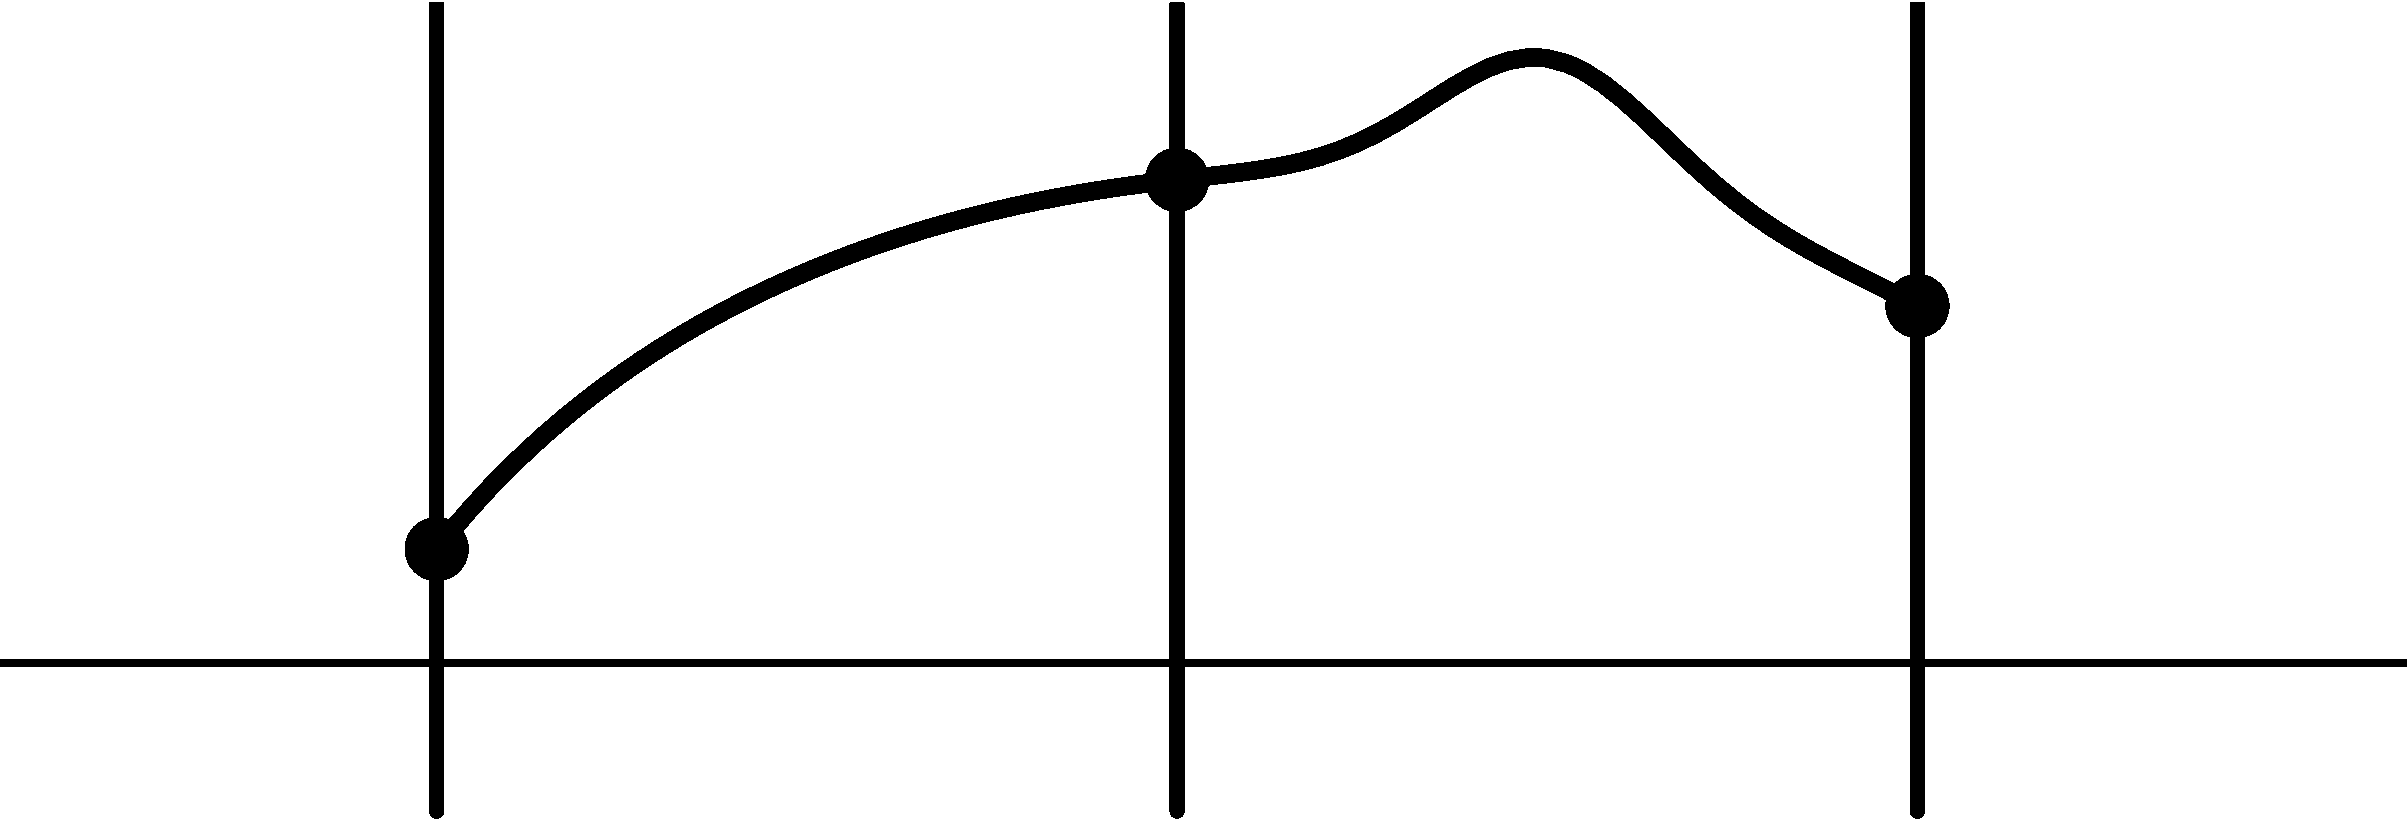
\includegraphics[width=6cm]{Images/proof}};
			\draw [color=black](0,.6) node[anchor=north west] {$l_n(\t_0)$};
			\draw [color=black](-2.4,-1.05) node[anchor=north west] {$\t_0-\delta$};
			\draw [color=black](1.3,-1.05) node[anchor=north west] {$\t_0+\delta$};
			\draw [color=black](-0.3,-1.05) node[anchor=north west] {$\t_0$};
			\end{tikzpicture}
		\end{center}
		Protože $l_n(\t)$ je na~intervalu $(\t_0-\delta,\t_0+\delta)$ diferencovatelná (tedy i~spojitá), pak pro~$\forall\delta$ s~pravděpodobností $\PP_{\t_0}\to1$ existuje $\widehat{\t}_n$ jako řešení $l_n'(\widehat{\t}_n)=0$, které se~nachází v~intervalu $(\t_0-\delta,\t_0+\delta)$ a~je tedy konzistentní pro~$\t_0$.
	\end{proof}
\end{theorem}

\begin{example}[Původně ze~SME]
	Mějme $X_1,...,X_n~iid~\n{\mu,\sigma^2},~\hat{\mu}_\txt{ML}=?,~\widehat{\sigma}^{2}_\txt{ML}=?$
	\[
	\begin{split}
	L(\mu,\sigma^2)&=\prod\limits_{i=1}^n f_{X_i}(x_i,\mu,\sigma^2)=\prod\limits_{i=1}^n \frac{1}{\sqrt{2\pi\sigma^2}}\e{-\frac{(x_i-\mu)^2}{2\sigma^2}}=(2\pi\sigma^2)^{-\frac{n}{2}}\e{-\frac{1}{2\sigma^2}\sumjn(x_j-\mu)^2}.\\
	l(\mu,\sigma^2)&=\ln L(\mu,\sigma^2)=-\frac{n}{2}\ln(2\pi)-\frac{n}{2}\ln\sigma^2 -\frac{1}{2\sigma^2}\sumjn(x_j-\mu)^2.\\
	\frac{\partial l}{\partial \mu}&=\frac{1}{\sigma^2}\sumjn(x_j-\mu)=0\qquad\qquad\qquad\Rightarrow\quad\widehat{\mu}=\frac{1}{n}\sumjn x_j =\oxnn, \\
	\frac{\partial l}{\partial (\sigma^2)}&=-\frac{n}{2}\frac{1}{\sigma^2}+\frac{1}{2\sigma^4}\sumjn(x_j-\mu)^2=0\quad \Rightarrow\quad \widehat{\sigma}^2=\frac{1}{n}\sumjn (x_j-\oxnn)^2.
	\end{split}
	\]
	$$ \frac{\partial^2 l}{\partial\mu^2}=-\frac{n}{\sigma^2},\qquad\frac{\partial^2 l}{\partial\mu\partial\sigma^2}=-\frac{1}{\sigma^4}\sumjn (x_j-\mu),\qquad\frac{\partial^2 l}{\partial(\sigma^2)^2}=\frac{n}{2}\frac{1}{\sigma^4}-\frac{1}{\sigma^6}\sumjn(x_j-\mu)^2, $$
	
	$$ \fisher_{12}=\fisher_{21}=-\EE{ -\frac{1}{\sigma^4}\sumjn (X_j-\mu) }=\frac{1}{\sigma^4} \Br{\sumjn (\underbrace{\E X_j}_{=\mu}-\mu)} =0, $$
	$$  \fisher_{11}=\frac{n}{\sigma^2}, \qquad  \fisher_{22}=-\frac{n}{2}\frac{1}{\sigma^4}+\frac{1}{\sigma^6}\sumjn \underbrace{\E (X_j-\mu)^2}_{\sigma^2}=\frac{n}{2\sigma^4}. $$
	Fisherova informační matice má tedy tvar $\fisher_n=\matice{
		\frac{n}{\sigma^2}}{0}{0}{\frac{n}{2\sigma^4}}=n\matice{
		\frac{1}{\sigma^2}}{0}{0}{\frac{1}{2\sigma^4}}=n\fisher_1(\mu,\sigma^2)$.
	Speciálně pro~odhad jednorozměrného paramentru $\mu$ získáme odhad $\widehat{\mu}_\txt{ML}=\Oxn$, pro~který plyne asymptotická normalita:
	$$ \sqrt{n}(\Oxn-\mu)\Dto \NN(0,\underbrace{\sigma^2}_{\inv{\fisher_1}(\mu)}). $$	
	V případě náhodného výběru z~normálního rozdělení se~tedy jedná o~přesné rozdělení $\Oxn$ (nejenom asymptotické), protože víme, že
	$$ \Oxn\sim\n{\mu,\frac{\sigma^2}{n}},\quad \Oxn-\mu\sim\n{0,\frac{\sigma^2}{n}},\quad \sqrt{n}(\Oxn-\mu)\sim\n{0,\sigma^2}. $$

\end{example}
	\begin{center}
	\begin{tikzpicture}
	\node[inner sep=0pt] (pic) at (0,0)
	{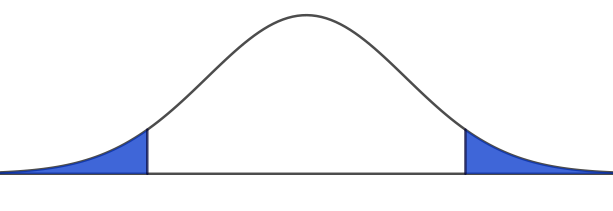
\includegraphics[width=6cm]{Images/KK}};
	\draw [color=black](0.6,1.) node[anchor=north west] {$f_{T^\ast}$};
	\draw [color=blue!40!black](-2.1,-0.75) node[anchor=north west] {$-K_1'$};
	\draw [color=blue!40!black](1.2,-0.75) node[anchor=north west] {$K_1'=u_{1-\frac{\alpha}{2}}$};
	\draw [color=blue!40!black](-2.2,0.2) node[anchor=north west] {$\frac{\alpha}{2}$};
	\draw [color=blue!40!black](1.7,0.2) node[anchor=north west] {$\frac{\alpha}{2}$};
	\end{tikzpicture}
\end{center}
\chapter{Testování statistických hypotéz}

\section{Základní strategie TSH}
Cílem testování statistických hypotéz je rozhodnout, zda jsme na~základě nějakého experimentu schopni ověřit platnost určitého vysloveného tvrzení (hypotézy) na~úrovni celé populace, případně parametru $\t$ s~touto populací spojeného. Můžeme tak například posoudit, jestli výsledky maturitních testů z~matematiky závisí na~pohlaví a~na~místě narození studentů.
Experiment provádíme na~jednotlivých jedincích,  přičemž často máme k~dispozici tzv. pokusnou a~kontrolní skupinu. Příkladem toho může být například dvojitě zaslepený experiment (\textit{double-blind experiment}), pomocí něhož zkoumáme účinky daného léku. Zde máme dvě skupiny pacientů - první skupině podáváme lék, který chceme otestovat, a~té druhé placebo, případně jiný medikament. Zároveň ale ani pacienti, ani lékaři, neví, které skupině jaký typ léku aplikujeme. Výsledky se~pak zpracují právě užitím testování statistických hypotéz.

Mějme nějaký objekt/subjekt O~a~jeho stav $S\in\mathscr{S}=\mathscr{S}_0+\mathscr{S}_1$ (disjunktní sjednocení $\mathscr{S}_0\cup\mathscr{S}_1$). Testujeme hypotézu
$H_0:\text{ O~je ve~stavu z~}\mathscr{S}_0$ oproti~$H_1:\text{O je ve~stavu z~}\mathscr{S}_1$. Máme-li náhodnou veličinu $X\sim f\in\mathcal{F}$ spojenou se~stavy objektu O~způsobem, že $\mathscr{S}\leftrightarrow\mathcal{F}$ jsou ve~vzájemně jednoznačném vztahu, potom úlohu reformulujeme na
	$$ \hypothesiswide{X\sim f\in\mathcal{F}_0\subset \mathcal{F}}{X\sim f\in \mathcal{F}_1=\mathcal{F}\dotminus\mathcal{F}_0}.$$
	Při případné parametrizaci modelu musíme dbát na~identifikovatelnost rodiny $\mathcal{F}$


\begin{define}
	Mějme populaci $\Omega$ a~na~ní vlastnost $X\sim\FF$, kde \mbox{$\FF\in\mathcal{F}$}. Označme $\t=\t(\FF)$ parametr modelu, který nás zajímá, kde $\t\in\Theta\subset\R^k$. Označme $H_0:\t\in\Theta_0$ jako \textbf{základní nulovou hypotézu} (\textit{null hypothesis}) a~ $H_1:\t\in\Theta_1$, kde \mbox{$\Theta_1=\Theta\setminus\Theta_0$}, jako \textbf{alternativní hypotézu}. 
\end{define}

Nulová hypotéza $H_0$ může označovat "původní stav", tedy že zkoumaná věc se~nezměnila, nebo že je lepší, než nějaký alternativní stav z~hypotézy $H_1$. Ta naproti~tomu  většinou doplňkově vyvrací platnost nulové hypotézy $H_0$, např. že nový lék funguje lépe než starý, nebo že alternativní rozdělení odpovídá naměřeným datům více, než distribuce deklarovaná v~$H_0$. O~zamítnutí $H_0$, resp. přijetí, rozhodujeme na~základě dostupného náhodného výběru $\X=(X_j)_{j=1}^n$ pořízeného v~rámci  zvoleného experimentu.

\begin{example}
	Hypotézou $H_0$ může být například to, že náhodný výběr pochází z~normálního rozdělení, nebo že 2 náhodné výběry pochází ze~stejného rozdělení, případně že mají alespoň stejnou střední hodnotu nebo rozptyl.
	Máme-li dvě výrobní metody a~k~nim příslušné náhodné výběry $X_1,...,X_n\sim\n{\mu_1,\sigma_1^2}$ a~$Y_1,...,Y_m\sim\NN(\mu_2,\sigma_2^2)$, můžeme zkoumat například to, jestli platí $H_0:\mu_1=\mu_2$ (výrobní metody jsou ve~své střední hodnotě stejné), versus $H_1:\mu_1<\mu_2$ (nová metoda č.1 ($X_j$) je lepší, než původní metoda č.2 ($Y_j$)).
\end{example}
\begin{define}
	Definujeme $\rhn$ jako jev představující \textbf{zamítnutí} $H_0$ (\textit{rejection}) a~$\rhno$ jako \textbf{přijetí} $H_0$ (\textit{acception}). Pak \textbf{kritickou funkci testu} definujeme jako pravděpodobnost, že zamítneme $H_0$ na~základě naměřených dat $\textbf{x}$, tzn. $$\crossedphi(\textbf{x}):=\PP(\rhn|\X=\textbf{x})\in[0,1],\quad\text{pro~}\forall\textbf{x}\in\mathcal{X},$$
	kde $\mathcal{X}$ je tzv. \textbf{výběrový prostor}, $\mathcal{X}=\{ \textbf{x}\in\R^n:\exists\omega\in\Omega,~\X(\omega)=\textbf{x} \}$. Dále definujeme pro~test $\hypothesis{\t\in\Theta_0}{\t\in\Theta_1},~\Theta=\Theta_0+\Theta_1$, funkci
	\[\begin{split}
	\beta_\crossedphi(\t)&:=\E_\t[\crossedphi(\X)]=\E_\t[\PP(\rhn|\X=\textbf{x})]=\begin{array}{|l|}
	\PP(A)=\int\limits_{A}1\d \PP=\int\limits_{\Omega}\Identita{A}\d\PP=\E[\Identita{A}]\\ A=\{\rhn|\X=\textbf{x}\} 
	\end{array}=\\&=\E_\t\big[\E[\Identita{\rhn}|\X=\textbf{x}]\big]\equal{\E[\E[X|Y]]=\E X}\E_\t[\Identita{\rhn}]=\PP_\t(\rhn),\quad\text{pro } \forall\t\in\Theta . 
	\end{split}\]
	Funkce $\silofunkce{1}$, tedy zúžení $\beta_\crossedphi$ z~$\Theta$ na~obor $\Theta_1$, se~nazývá \textbf{silofunkce testu} $\crossedphi$.
\end{define}
~\\
Pokud testujeme hypotézu $H_0$ oproti~$H_1$, mohou nastat 4 navzájem se~vylučující situace:\begin{center}
	\begin{tabular}{|l|c|c|}
		\hline 
		& \textbf{Zamítáme $H_0$} & \textbf{Nezamítáme $H_0$} \\ 
		\hline 
		\textbf{$H_0$ platí} & Nastává chyba I. druhu  & Správný výsledek \\ 
		\hline 
		\textbf{$H_0$ neplatí} & Správný výsledek & Nastává chyba II. druhu\\ 
		\hline 
	\end{tabular} 
\end{center}
Chybu I. druhu považujeme za~kritickou (tu horší) chybu. Pravděpodobnost chyby I. druhu vyjadřuje právě funkce $\silofunkce{0}$, což je zúžení $\beta_\crossedphi$ z~$\Theta$ na~obor $\Theta_0$. Právě tuto pravděpodobnost budeme chtít mít pod~kontrolou, tzn. pro~vhodně malé zvolené číslo $\alpha\in(0,1)$ požadujeme, aby celé zúžení $\silofunkce{0}$ bylo stejnoměrně pod~zadanou hranicí $\alpha$. 
Číslo $\alpha$ nazýváme \textbf{hladina významnosti} testu $H_0$ versus $H_1$ a~požadujeme tedy, aby $\sup\limits_{\t\in\Theta_0}\beta_\crossedphi(\t)\leq \alpha.$


Pravděpodobnost chyby II. druhu vyjadřuje funkce $1-\silofunkce{1}$ a~budeme se~ji snažit minimalizovat za~vazební podmínky $\silofunkce{0}\leq \alpha$ na~chybu I. druhu.

\begin{figure}[h]
	\centering
	\begin{tikzpicture}
	\node[inner sep=0pt] (pic) at (0,0)
	{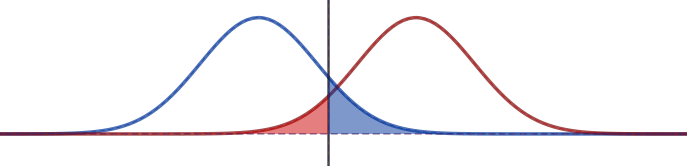
\includegraphics[width=10cm]{Images/hypothesis}};
	\draw [color=blue!20!black](-6.55,1.0) node[anchor=north west] {Alternativní hypotéza $H_1$};
	\draw [color=red!40!black](2.05,1.0) node[anchor=north west] {Nulová hypotéza $H_0$};
	\draw [color=black](-0.65,-0.35) node[anchor=north west] {$\alpha$};
	\draw [color=black](-2.6,1.75) node[anchor=north west] {Volená hranice pro~rozhodnutí mezi~$H_0$ a~$H_1$};
	\draw [color=black](-0.25,-0.25) node[anchor=north west] {$\beta$};
	\draw [color=black](-3.5,-1) node[anchor=north west] {Zamítáme $H_0$};
	\draw [color=black](1,-1) node[anchor=north west] {Nezamítáme $H_0$};
	\end{tikzpicture}
	\caption{Porovnání hypotéz pro~případ jednoduché $H_0$ (jeden stav) oproti~jednoduché $H_1$ (druhý alternativní stav).}
	\label{fig:grafik}
\end{figure}

Shrňme strategii testování $\hypothesis{\t\in\Theta_0}{\t\in\Theta_1}$ v~následující sekci.
\section{UMP testy pro~parametr $\t=\t(\FF)$}
\begin{define}[UMP strategie testování $H_0$ vs. $H_1$] Hledáme takovou optimální kritickou funkci testu $\Phiast$, aby při~zvolené hladině významnosti $\alpha\in(0,1)$ byla pravděpodobnost chyby II. druhu minimální, tzn. aby pro~$\forall\t\in\Theta_1$ bylo $\beta_{\Phiast}(\t)$ stejnoměrně na~$\Theta_1$ \textbf{maximální silou testu}, za~podmínky, že pravděpodobnost chyby I. druhu bude stále (stejnoměrně na~$\Theta_0$) pod~hranicí $\alpha$, tzn. $$\forall\t\in\Theta_0,~\beta_{\Phiast}(\t)\leq\alpha.$$
	Číslo $\sup\limits_{\t\in\Theta_0}\beta_{\Phiast}(\t)$ se~nazývá \textbf{hladina testu} (\textit{size of test $\Phiast$}) a~v~praxi může být ostře pod~nastavenou hranicí \textbf{hladiny významnosti} testu $\alpha$ (\textit{significance level $\alpha$}). 
	
	Konkrétní hodnotu $\beta_{\Phiast}(\t)$ pro~$\t\in\Theta_1$ nazýváme \textbf{síla testu} $\Phiast$ pro~dané $\t\in\Theta_1$, celé zúžení $\silofunkceast{1}$ pak nazýváme \textbf{silofunkce} testu $\Phiast$.
	
	Pokud takový test $\Phiast$ splňující uvedené podmínky existuje, nazýváme ho stejnoměrně nejsilnějším testem $H_0$ oproti~$H_1$, ozn. \textbf{UMP test} (\textit{uniformly most powerful test}). Situaci UMP ilustruje obrázek \ref{fig:UMP}.

\end{define}
	\begin{figure}[h]
	\centering
	\begin{tikzpicture}[scale=1.4]
	\node[inner sep=0pt] (pic) at (0,0)
	{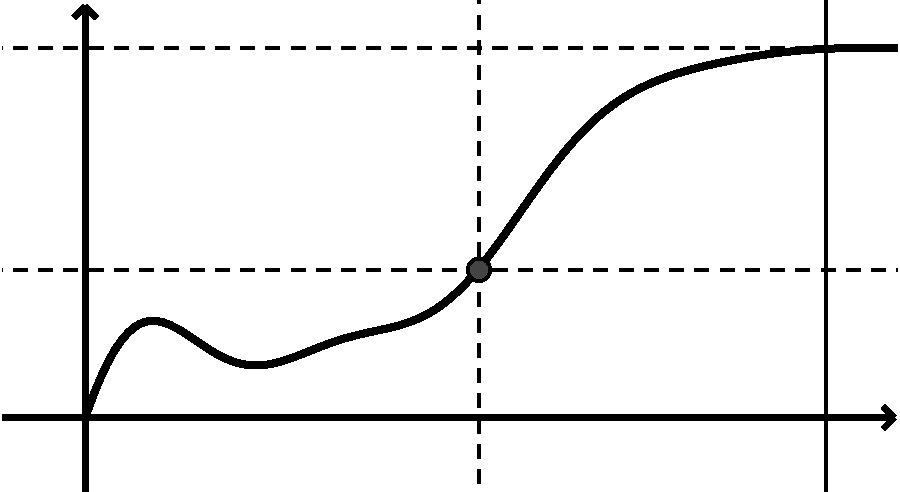
\includegraphics[width=6.0cm]{Images/test}};
	\draw [color=black](0.75,0.80) node[anchor=north west] {$\beta_\crossedphi(\t)$};
	\draw [color=black](-2.1,-0.85) node[anchor=north west] {$0$};
	\draw [color=black](-1.2,-0.9) node[anchor=north west] {$\Theta_0$};
	\draw [color=black](0.7,-0.9) node[anchor=north west] {$\Theta_1$};
	\draw [color=black](2.15,-0.62) node[anchor=north west] {$\t$};
	\draw [color=black](0.1,-0.1) node[anchor=north west] {$\sup\limits_{\t\in\Theta_0}\beta_\crossedphi$};
	\draw [color=black](-2.0,1.55) node[anchor=north west] {$\beta_\crossedphi$};
	\draw [color=black](-2.1,0.95) node[anchor=north west] {$1$};
	\draw [color=black](-2.1,0.2) node[anchor=north west] {$\alpha$};
	\end{tikzpicture}
	\caption{UMP model testování $\hypothesis{\t\in\Theta_0}{\t\in\Theta_1}$ na~hladině $\alpha$.}
	\label{fig:UMP}
\end{figure}
\begin{remark} Ještě lepší strategií by bylo hledat test $\crossedphi$, který minimalizuje stejnoměrně oba druhy chyb I. a~II. najednou. To však obecně nelze splnit, protože bohužel platí, že pokud se~snažíme snížit pravděpodobnost chyby jednoho druhu, pak pravděpodobnost druhé chyby roste. Tedy chyby I. a~II. druhu jsou komplementární, a~proto musíme volit určitou formu kompromisu (viz. definice UMP testu $\Phiast$). 
\end{remark}
\begin{define}	Pokud $\Theta_0$ je jednoprvková (1 stav), pak $H_0$ nazveme \textbf{jednoduchá} hypotéza (\textit{simple}), v~opačném případě je $H_0$ \textbf{složená} hypotéza (\textit{composite}). Totéž platí pro~$\Theta_1$ a~$H_1$ alternativu.
\end{define}
UMP je tedy test, který má nejvyšší statistickou sílu $\beta$ na~celém $\Theta_1$ $(H_1)$ mezi~všemi možnými testy pod~zadanou hranicí $\alpha$ pro~chybu I. druhu na~$\Theta_0$ $(H_0)$. Je taky dobré si uvědomit, že $\beta$ je pravděpodobnost, že nenastává chyba II. druhu. Takovýto optimální test nutně nemusí existovat. Pokud však existuje, je možné ho pro~speciální případ jednoduché $H_0$ a~jednoduché $H_1$ nalézt pomocí Neyman-Pearsonova lemmatu, které bude uvedeno dále v~sekci \ref{NPL}. 

\begin{define}
	Pokud uvažujeme kritickou funkci ve~tvaru $$\crossedphi(\textbf{x})=\begin{cases}
	1 & \textbf{x}\in W\subset\R^n, \\ 0 & \text{jinak},
	\end{cases}$$ pak $W$ nazveme \textbf{kritický obor testu} (\textit{critical region}). Je to tedy obor naměřených hodnot, při~kterém zamítáme $H_0$. Tomuto tvaru testu se~říká \textbf{neznáhodněný test} a~o~přijetí $H_0$ rozhodujeme následovně: \[
	\begin{split}
	\text{nastává jev }\{\X\in W\} ~&\Rightarrow~\text{zamítáme }H_0, \\ \text{nastává opačný jev }\{\X\notin W\} ~&\Rightarrow~\text{nezamítáme }H_0. 
	\end{split}
	\]\end{define} 
Kritický obor $W$ musí opět splňovat podmínku omezenosti pravděpodobnosti chyby I. druhu ve~tvaru $$ \PP_\t\br{(X_1,...,X_n)\in W}\leq \alpha,~\forall\theta\in\Theta_0, $$ pro~zadanou hladinu významnosti testu $\alpha\in(0,1)$. Příležitostně budeme pro~kritický obor proto užívat označení $W_\alpha$.

Pro stejnoměrně optimální UMP test $\Phiast$ pak odpovídající kritickou oblast značíme $W^\ast$ a~nazýváme ji \textbf{UMP kritickou oblastí testu} (\textit{UMP critical region - UMPCR}).
Pokud tedy $ (x_1,...,x_n)\in W^\ast$, pak zamítneme $H_0$. Opět příležitostně označíme $\txt{UMP}_\alpha,~\Phiast_\alpha$, nebo $W_\alpha^\ast$.

\section{Neyman-Pearsonovo lemma (N-PL)}\label{NPL}
Nyní už přichází na~řadu \textbf{Neyman-Pearsonovo lemma}, které nám umožní najít nejlepší možný test $\Phiast$ pro~případ jednoduché hypotézy $H_0$ (1 stav) oproti~jednoduché alternativě $H_1$ (také pouze 1 stav).
\begin{theorem}[Neyman-Pearsonovo lemma]
	Mějme dvě hypotézy
	\mbox{$ \hypothesis{\t=\t_0}{\t=\t_1}$} a~číslo $\alpha\in(0,1)$ jako hladinu významnosti testu. Označme nyní hustotu pravděpodobnosti \mbox{$f_0:=f(\textbf{x},\t_0)$} a~ $f_1:=f(\textbf{x},\t_1)$ obě vzhledem ke~vhodné dominující míře $\lambda$. Pak existuje $K>0$ a~UMP test $\Phiast$ ve~tvaru 
	$$ \Phiast(\textbf{x})=\begin{cases}
	1 & f_1>Kf_0,\\\gamma&f_1=Kf_0,\\0&f_1<Kf_0,
	\end{cases}~~~~\text{tak, že $\beta_{\Phiast}(\t_0)=\alpha$.} $$
	Pokud $\crossedphi$ je nějaký jiný UMP test na~hladině $\alpha$, pak $\crossedphi$ je nutně stejného tvaru jako $\Phiast$ na~množině $\{ f_1\neq Kf_0 \}$. Výjimkou je situace, kdy existuje test $\crossedphi$ s~$\beta_\crossedphi(\t_1)=1$, přičemž \mbox{$\beta_\crossedphi(\t_0)<\alpha$}, což znamená, že test $\crossedphi$ nemůže dosáhnout zadané hranice $\alpha$ pro~svou pravděpodobnost chyby I. druhu tak, jako ji dosahuje test $\Phiast$.
	\begin{proof}Konstruktivní důkaz (nutno znát ke~zkoušce).
	\begin{enumerate}[a)]
	\item Nejprve zkonstruujeme nějaký test $\Phiast$ požadovaného tvaru. Definujeme \[
	\begin{split}
	\alpha(c)&:=\PP_{\t_0}(f_1>cf_0)=\PP_{\t_0}(f_1>cf_0\wedge f_0>0)=\PP_{\t_0}\Br{\frac{f_1}{f_0}>c}=1-\PP_{\t_0}\Br{\underbrace{\frac{f_1}{f_0}}_{Y\geq 0}\leq c}=\\&=1-\FF_Y(c).
		\end{split}
			\]
	Protože $\FF_Y$ je nějaká distribuční funkce jisté náhodné veličiny $Y$, pak $\alpha(c)$ je nerostoucí, zprava spojitá a~limitně se~chová jako $\lim\limits_{c\to-\infty}\alpha(c)=1$, $\lim\limits_{c\to+\infty}\alpha(c)=0$.	\begin{center}
				\begin{tikzpicture}[scale=1.1]
				\node[inner sep=0pt] (pic) at (0,0)
				{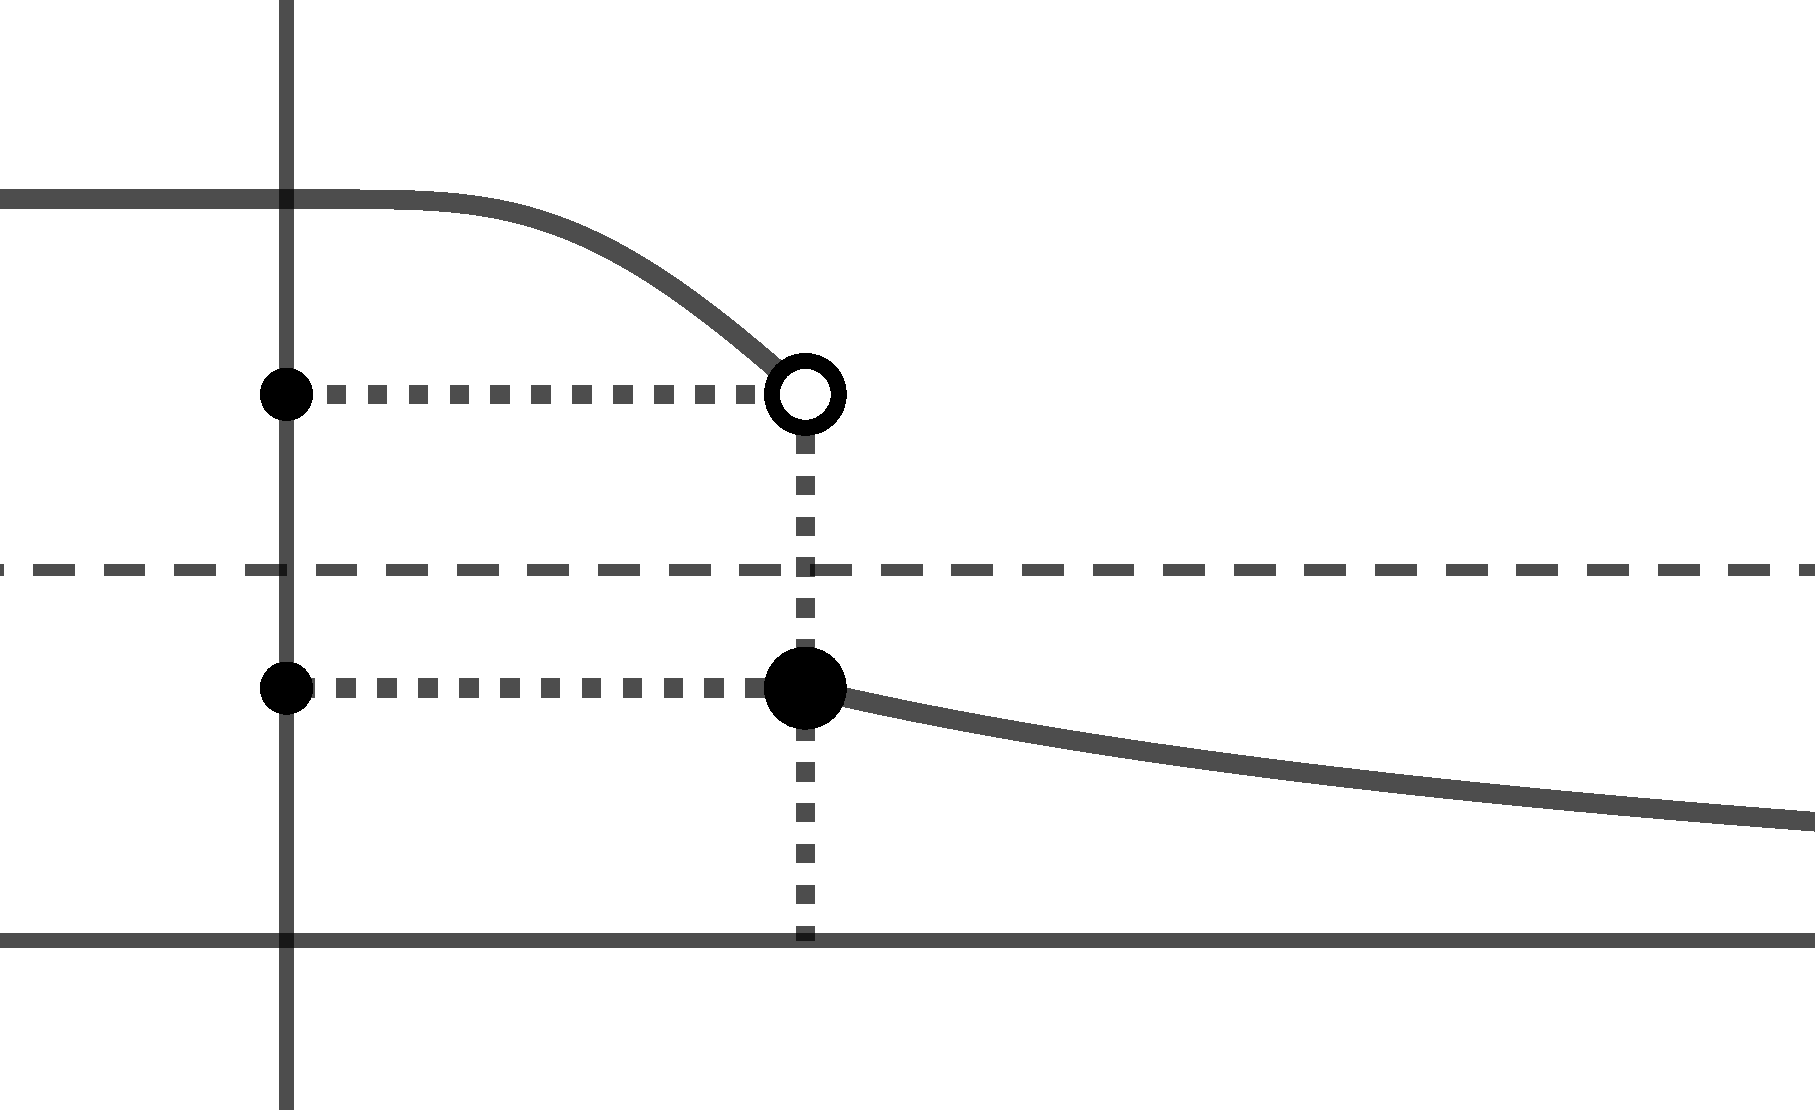
\includegraphics[width=5.5cm]{Images/lemma}};
				\draw [color=black](0.75,-0.05) node[anchor=north west] {$\alpha(c)$};
				\draw [color=black](1.95,0.4) node[anchor=north west] {$\alpha$};
				\draw [color=black](-2.2,-1.1) node[anchor=north west] {$0$};
				\draw [color=black](-0.5,-1.15) node[anchor=north west] {$c_0$};
				\draw [color=black](-2.2,1.55) node[anchor=north west] {$1$};
				\draw [color=black](-3.05,0.8) node[anchor=north west] {$\alpha(c_0-)$};
				\draw [color=black](-2.8,-0.2) node[anchor=north west] {$\alpha(c_0)$};
				\end{tikzpicture}
			\end{center}
			Pro $c_0$ takové, že $\alpha(c_0-)\geq \alpha\geq \alpha(c_0)$, definujeme  
			$$ \Phiast(\textbf{x}):=\begin{cases}
			1&f_1>c_0f_0,\\\gamma=\frac{\alpha-\alpha(c_0)}{\alpha(c_0-)-\alpha(c_0)}&f_1=c_0f_0,\\0&f_1<c_0f_0,
			\end{cases} $$ kde $\alpha(c_0-)$ značí $\lim\limits_{c\to c_0-}\alpha(c)$.
			V případě, že $\alpha(c)$ je spojitá v~$c_0$, pak číslo $\gamma$ je nedefinováno ($\frac{0}{0}$). To však nevadí, protože v~tomto případě platí
			$$ 0= \alpha(c_0-)-\alpha(c_0)=1-\alpha(c_0)-\br{1-\alpha(c_0-)}=\underbrace{\PP_{\t_0}\Br{\frac{f_1}{f_0}\leq c_0}}_{F_Y(c_0)}-\underbrace{\PP_{\t_0}\Br{\frac{f_1}{f_0}< c_0}}_{F_Y(c_0-)}=\PP_{\t_0}\Br{\frac{f_1}{f_0}=c_0}, $$ a~tedy vidíme, že množina $\{ f_1=c_0f_0\}$ má nulovou pravděpodobnostní míru. To znamená, že test $\Phiast$ je definován jednoznačně $s.j.~\PP_{\t_0}$. Hladina tohoto testu $\Phiast$ je
			\[
			\begin{split}
			\beta_{\Phiast}(\t_0)&=\E_{\t_0}\crossedphi(\X)=1\cdot \PP(\Phiast=1)+\gamma\PP(\Phiast=\gamma)+0\cdot\PP(\Phiast=0)=\\&=\underbrace{\PP(f_1>c_0f_0)}_{\alpha(c_0)}+\frac{\alpha-\alpha(c_0)}{\alpha(c_0-)-\alpha(c_0)}\cdot\underbrace{\PP(f_1=c_0f_0)}_{\alpha(c_0-)-\alpha(c_0)}=\alpha.
			\end{split}
			\]
			\item Nyní ukážeme, že zkonstruovaný test $\Phiast$ je UMP testem. Nechť $\Phiast$ je test z~předchozí části důkazu a~$\crossedphi$ je libovolný jiný test na~hladině významnosti $\alpha$, tzn. $\beta_{\crossedphi}(\t_0)\leq \alpha$. Chceme ukázat, že $\beta_{\Phiast}(\t_1)-\beta_{\crossedphi}(\t_1)\geq0$.
			\[
			\begin{split}
			&\beta_{\Phiast}(\t_1)-\beta_{\crossedphi}(\t_1)=\E_{\t_1}[\Phiast(\X)-\crossedphi(\X)]=\int\limits_{\R^n}(\Phiast-\crossedphi)f_1(\textbf{x})\d\textbf{x}=\\
			&=\underbrace{\int\limits_{S^+:=\{ \Phiast-\crossedphi>0 \}}(\Phiast-\crossedphi)f_1\d\textbf{x}}_{\textbf{x}\in S^+\Rightarrow~\Phiast>0~\Rightarrow~f_1\geq c_0f_0}+\underbrace{\int\limits_{S^-:=\{ \Phiast-\crossedphi<0 \}}(\Phiast-\crossedphi)f_1\d\textbf{x}}_{\textbf{x}\in S^-\Rightarrow~\Phiast<1~\Rightarrow~ f_1\leq c_0f_0}+\underbrace{\int\limits_{\{ \Phiast-\crossedphi=0 \}}(\Phiast-\crossedphi)f_1\d\textbf{x}}_{=0}\geq\\
			&\geq
			\int\limits_{S^+}(\Phiast-\crossedphi)c_0f_0\d\textbf{x}+ \int\limits_{S^-}(\Phiast-\crossedphi)c_0f_0\d\textbf{x}=c_0\underbrace{\int\limits_{\R^n}(\Phiast-\crossedphi)f_0\d\textbf{x}}_{\E_{\t_0}(\Phiast-\crossedphi)}=c_0\br{\underbrace{\beta_{\Phiast}(\t_0)}_{=\alpha}-\underbrace{\beta_{\crossedphi}(\t_0)}_{\leq\alpha}}\geq 0. 
			\end{split}
			\] Z~toho vyplývá, že síla testu $\Phiast$ je větší, než síla testu $\crossedphi$. Konstantu $c_0$ z~důkazu ztotožňujeme s~$K>0$ ze~znění věty.
		\end{enumerate}
	\end{proof}
\end{theorem}
\begin{dusl}\label{dusledek} Pokud platí, že $\PP_{\t_0}(f_1=Kf_0)=0$, pak můžeme psát
	$$ \Phiast=\begin{cases}
	1&x\in W^\ast=\{ f_1\geq Kf_0 \},\\0& x\in (W^\ast)^c=\{f_1<Kf_0\}.
	\end{cases} $$ Tedy v~případě, že hranice $\{f_1= Kf_0\} $ je nulové $\PP_{\t_0}$ míry, potom existuje neznáhodněný test s~UMP kritickou oblastí $W^\ast$ pro~testování $H_0$ versus $H_1$, přičemž pravděpodobnost chyby I. druhu je přímo rovna požadované signifikanci $\alpha$,  $\beta_{W^\ast}(\t_0)=\alpha$, zatímco síla testu $\beta_{W^\ast}(\t_1)$ je maximální možná.
\end{dusl}
\begin{example}
	Neyman-Pearsonovo lemma se~zpravidla používá pro~tzv. jednoduché testy, což znamená, že je testovaný parametr zadaný konkrétní jednou hodnotou. Příkladem může být třeba testování hypotéz pro~parametry $\n{\mu,\sigma^2}$ typu 
$$ \hypothesis{\mu=\mu_0}{\mu=\mu_1\neq\mu_0~(\text{resp. }\mu\gtrless\mu_0)}. $$
 Pro~složené testy, např. typu
$$ \hypothesis{\sigma^2\geq7}{\sigma^2< 7},\quad\text{nebo }\hypothesis{\mu\leq\mu_0}{\mu>\mu_0},  $$ ani jiné podobně zadané testy, optimální $\txt{UMP}_\alpha$ test nemusí obecně existovat a~jsou nutné dodatečné podmínky (viz následující sekce).
\end{example}

\section{Složené hypotézy a~MLR systémy}
\subsection*{Postup použití N-PL v~praxi pro~test z~důsledku \ref{dusledek}.}Hledáme takový test $\Phiast$ tvaru 
$$ \Phiast(\textbf{x})=\begin{cases}
1&\textbf{x}\in\{f_1\geq Kf_0\}=W^\ast\text{ ... UMP CR},\\0&\textbf{x}\in\{f_1<Kf_0\}=(W^\ast)^c,
\end{cases} $$
pro který je dosažena hladina testu $\beta_{\Phiast}(\t_0)=\alpha$, přičemž síla (silofunkce) testu $\beta$ je optimální.
\begin{enumerate}[1)]
	\item Nejdříve najdeme \textbf{tvar} $W^\ast$ jako řešení nerovnice $f_1\geq Kf_0$. Získáme ho v~nějakém tvaru $W^\ast=\{ T(\textbf{x})\geq K' \}$, resp. $W^\ast=\{ T(\textbf{x})\leq K' \}$, s~blíže nespecifikovanou volnou konstantou $K'$, tedy 
	$$\{f_1\geq Kf_0\}\sim\{T(\X)\geq K' \},$$ resp.$$\{f_1\geq Kf_0\}\sim\{T(\X)\leq K' \},$$
	kde $T(\X)$ se~nazývá \textbf{testovací statistika}.
	\item Konkrétní hodnotu $K'$ pak určíme z~rovnice  $\PP_{\t_0}\br{T(\X)\geq K'}=\alpha$, resp.  $\PP_{\t_0}\br{T(\X)\leq K'}=\alpha$. K~vyřešení této nerovnosti však nutně potřebujeme umět vyjádřit $\PP_{\t_0}(T\geq K')$, resp. \mbox{$\PP_{\t_0}(T\leq K')$} za~předpokladu platnosti hypotézy $H_0$, tzn. při~$\t_0$. Odvození rozdělení $T(\X)$ při~$\t_0$ se~říká "distributional problem"~testování hypotéz a~jde o~stěžejní část úspěšné aplikace.
	\item V~případě, že $H_1$ je složená, tzn. $H_1:\t\in\Theta_1$, postupujeme takto:
	volíme $\t_1\in\Theta_1$ libovolně pevně a~testujeme hypotézu
	$ \hypothesis{\t=\t_0}{\t=\t_1\text{ na~hladině }\alpha.} $
	Z Neyman-Pearsonova lemmatu existuje $\txt{UMP}_\alpha$ test $\Phiast$, případně UMPCR $W^\ast$. Pokud tento $\Phiast$, případně $W^\ast$, nezávisí na~volbě $\t_1$, máme finální $\txt{UMP}_\alpha$ test při~složené alternativě $H_1$.
	\item  Pokud i~$H_0$ je složená, tzn. $H_0:\t\in\Theta_0$, pak, pokud to lze, ještě navíc ukážeme, že  $\sup\limits_{\t\in\Theta_0}\beta_{\Phiast}(\t)\leq\alpha$, tzn., že $\forall\t_0'\in\Theta$, platí, že $\beta_{\Phiast}(\t_0')\leq\alpha$. Průchodnost bodů 3) a~4) zajišťuje například následující koncept MLR.
\end{enumerate}

\begin{define}
	Systém hustot $\mathcal{F}$ se~nazývá  \textbf{MLR} (\textit{Monotone likelihood ratio}), pokud \newline $\exists T(\textbf{x}):\R^n\to\R^1$ tak, že pro~$\forall\t_0<\t_1$ platí, že $\frac{f_1}{f_0}$ je monotonní funkcí statistiky $T(\textbf{x})$, tzn. \mbox{$\frac{f_1}{f_0}=g\br{T(\textbf{x})}$}, kde $g$ je monotonní. Podíl $\frac{f_1}{f_0}=\frac{L(\t_1)}{L(\t_0)}$ se~nazývá \textbf{věrohodnostním poměrem} (\textit{likelihood ratio}), ozn. $\mathrm{LR}(\textbf{x}),~\textbf{x}\in\mathcal{X}$.
\end{define}
\begin{remark}
	Pokládáme $\frac{f_1}{f_0}=+\infty$, pokud $f_1>0,~f_0=0$. Pro~$f_1=0$ a~$f_0=0$ výraz nedefinujeme. Monotonii vyžadujeme pouze tam, kde je výraz $\mathrm{LR}(\textbf{x})$ definován.
\end{remark}
\begin{theorem}\label{vetaUMP} Mějme rostoucí MLR systém hustot $\mathcal{F}$ se~statistikou $T(\X)$. Testujeme hypotézu \\
	\mbox{$ \hypothesis{\t\leq\t_0}{\t>\t_0}$}, $\t\in\R^1 $, tzv. jednostrannou hypotézu oproti~jednostranné alternativě, na~zadané hladině $\alpha\in(0,1)$.
	Pak existuje $\txt{UMP}_\alpha$ test $\Phiast$ ve~tvaru $$ \Phiast(\textbf{x})=\begin{cases}
	1 & T(\textbf{x})>K, \\ \gamma &T(\textbf{x})=K, \\ 0&T(\textbf{x})<K,
	\end{cases} $$ přičemž $K$ a~$\gamma$ jsou určeny podmínkou $\beta_{\Phiast}(\t_0)=\alpha$, tzn.  $\E_{\t_0}[\Phiast(\X)]=\alpha$, tedy $$\PP_{\t_0}\br{T(\X)>K}+\gamma \PP_{\t_0}\br{T(\X)=K}+0\cdot \PP_{\t_0}\br{T(\X)<K}	=\alpha.$$
	Pro případ klesajícího MLR systému $\mathcal{F}$ stačí v~tvrzení zaměnit nerovnosti za~opačné.
	\begin{proof} Důkaz provedeme speciálně pro~ostře rostoucí MLR systém $\mathcal{F}$.
		\begin{enumerate}[a)]
			\item Nejprve testujeme $\hypothesis{\t=\t_0}{\t>\t_0}$. Pro~tento účel zvolíme libovolně pevně $\t_1>\t_0$ a~testujeme $\hypothesis{\t=\t_0}{\t=\t_1}$.  Tím splníme překpoklady Neyman-Pearsonova lemmatu, podle něhož pak existuje UMP test $$ \Phiast(\textbf{x})=\begin{cases}
			1&f_1>K'f_0, \\ \gamma&f_1=K'f_0, \\ 0&f_1<K'f_0,
			\end{cases}  $$ tak, že $\beta_{\Phiast}(\t_0)=\alpha$. Nechť $\frac{f_1}{f_0}=g\br{T(\textbf{x})}$, kde $g$ je ostře rostoucí funkcí. Nyní upravíme podmínky do~tvaru
			$$ \left\{ \begin{array}{c}
			f_1>K'f_0	\\ f_1=K'f_0  \\ f_1<K'f_0
			\end{array}  \right\}\sim\left\{ \begin{array}{c}
			f_1/f_0>K'	\\ f_1/f_0=K'  \\ f_1/f_0<K'
			\end{array}  \right\}\sim\left\{ \begin{array}{c}
			T(\textbf{x})>\inv{g}(K')	\\ T(\textbf{x})=\inv{g}(K')  \\ T(\textbf{x})<\inv{g}(K')
			\end{array}  \right\}\sim\left\{ \begin{array}{c}
			T(\textbf{x})>K	\\ T(\textbf{x})=K  \\ T(\textbf{x})<K	\end{array}  \right\}, $$ kde  $K:=\inv{g}(K')$. Tvar testu $\Phiast$ je stejný nezávisle na~volbě $\t_1>\t_0$. Konstanty $K$ a~$\gamma$ jsou pak určeny z~rovnice $\beta_{\Phiast}(\t_0)=\alpha$, a~proto také nezávisí na~volbě $\t_1>\t_0$.		
			\item Vezmeme právě zkonstruované $\Phiast$ a~ukážeme, že pro~$\forall\t_0'<\t_0$ platí, že $\beta_{\Phiast}(\t_0')\leq \alpha$. Definujeme pomocný (čárkovaný) test $$H_0':\t=\t_0'~\text{vs.}~H_1':\t=\t_0.$$ Příslušný UMP test $H_0'$ z~N-PL má stejný tvar jako UMP $\Phiast$ zkonstruovaný v~předchozím bodě, ale na~hladině $\beta_{\Phiast}(\t_0')=\alpha'$. Jeho síla je pak rovna $\beta_{\Phiast}(\t_0)=\beta'$. 
			\item Ukážeme, že pro~UMP test $\Phiast$ platí $\alpha'\leq\beta'$. Volme test $\crossedphi(\textbf{x})=\alpha'$ pro~$\forall\textbf{x}\in\mathcal{X}$. Pak $\crossedphi$ je test $H_0'$ vs. $H_1'$ na~hladině $\alpha'$ se~silou $\alpha'$, která nemůže překročit sílu $\beta'$ UMP testu $\Phiast$, tzn. $\alpha'\leq \beta'$.
		\end{enumerate}
	\end{proof}
\end{theorem}
	\begin{example}\label{prikladek}
	Testujeme hypotézu  $H_0: \t\leq\t_0~\text{vs.}~H_1:\t>\t_0$ pro~exponenciální třídu hustot $$\mathcal{F}=\big\{ f(x,\t)=c(\t)h(x)\e{Q(\t)T(x)}:\t\in\Theta\subset\R^1 \big\}.$$ Pokud $Q(\t)$ je ryze rostoucí, resp. ryze klesající, pak $\mathcal{F}_n\equal{iid}\left\{ f(\textbf{x},\t)=\prod\limits_{i=1}^n f(x_i,\t) \right\}$ je MLR systém hustot se~statistikou $T(\textbf{x})=\sum\limits_{i=1}^n T(x_i)$. Z~věty \ref{vetaUMP} pak plyne konkrétní tvar $\txt{UMP}_\alpha$ testu $\Phiast$ pro~testování $H_0$ vs. $H_1$.
Díky této MLR exponenciální třídě hustot umíme najít stejnoměrně optimální UMP testy například pro~následující parametry specifických rozdělení:
\[
\begin{split}
H_0:p\leq p_0~\text{vs.}~H_1:p>p_0,&\quad\text{v~případě }X\sim\mathrm{Bi}(n,p),\\
H_0:\lambda\leq\lambda_0~\text{vs.}~H_1:\lambda>\lambda_0,&\quad\text{v~případě } X\sim\mathrm{Po}(\lambda),\\
\hypothesis{\t\leq\t_0}{\t>\t_0},&\quad\text{pro případ }X\sim\mathrm{Exp}(\t),\\
\hypothesis{\mu\leq\mu_0}{\mu>\mu_0},&\quad\text{při modelu }X\sim\NN(\mu,\sigma^2\text{ známé}),\text{ atp.}
\end{split}
\]
\end{example}
\section{Nestranné UMP testy (UMPU)}
V aplikacích TSH v~praxi vyvstává nutnost testovat další složitější hypotézy, jako například \[
	\begin{split}
	H_0:&~\t=\t_0~\text{vs.}~H_1:\t\neq\t_0,\quad\text{nebo} \\
	H_0:&~\t_1\leq \t\leq\t_2~\text{vs.}~H_1:\t\notin[\t_1,\t_2].
	\end{split}
	\]
	Pro takovéto případy, kdy alternativní hypotéza $H_1$ je tzv. oboustranná ($\t<\t_1$ nebo $\t>\t_2$), zpravidla neexistuje stejnoměrně nejsilnější $\txt{UMP}\alpha$ test $\Phiast$ na~hladině $\alpha$ a~jsme nuceni z~optimality UMP testu slevit. Zavedeme proto UMPU testy.
	
\begin{define}	
	Testujme $H_0:\t\in\Theta_0~\text{vs.}~H_1:\t\in\Theta_1$.
	Test $\crossedphi$ se~nazývá nestranný, pokud $\sup\limits_{\t\in\Theta_0}\beta_\crossedphi(\t)\leq \inf\limits_{\t\in\Theta_1}\beta_\crossedphi(\t)$.
\end{define}
\begin{theorem}\label{zobecneni}
	Každý UMP test $\Phiast$ je nestranný, tzn. $\silofunkceast{0}\leq\silofunkceast{1}$, tj. $$\sup\limits_{\t\in\Theta_0}\beta_{\Phiast}(\t)\leq\inf\limits_{\t\in\Theta_1}\beta_{\Phiast}(\t).$$
	\begin{proof}
		Volme $\crossedphi(\textbf{x})=\widetilde{\alpha}=\sup\limits_{\t\in\Theta_0}\beta_{\Phiast}(\t)$ pro~$\forall\textbf{x}\in\mathcal{X}$. Pak
		\[
		\begin{split}
		\silofunkce{0}&=\E_{\t_0}\crossedphi(\X)=\widetilde{\alpha},~~~\forall\t_0\in\Theta_0,\quad\text{(hladina testu $\crossedphi$)} \\\silofunkce{1}&=\E_{\t_1}\crossedphi(\X)=\widetilde{\alpha},~~~\forall\t_1\in\Theta_1.\quad\text{(silofunkce testu $\crossedphi$)}
		\end{split}
		\] 
		Podle předpokladu je $\Phiast$ UMP, a~tedy jeho silofunkce je stejnoměrně na~$\Theta_1$ vyšší, než u~všech ostatních testů včetně testu $\crossedphi$. Proto platí, že $\beta_{\Phiast}(\t_1)\geq\widetilde{\alpha}$ pro~$\forall\t_1\in\Theta_1$. Věta \ref{zobecneni} zobecňuje výsledek z~bodu c) z~důkazu věty \ref{vetaUMP}.
	\end{proof}
\end{theorem}

\begin{define}
	Stejnoměrně nejsilnější test mezi~všemi nestrannými testy se~nazývá UMPU. (\textit{UMP Unbiased}).
\end{define}


\begin{theorem} \label{UMPU}
	Testujeme hypotézu	$H_0:\t=\t_0~\text{vs.}~H_1:\t\neq\t_0,$ kde $\t\in\Theta\subset\R^1$ a~$\t_0$ je vnitřním bodem $\Theta$, tedy , $\t_0\in\Theta^\circ$. Nechť $\mathcal{F} $ je exponenciální třída hustot z~příkladu \ref{prikladek} s~$Q(\t)$ ryze rostoucí a~diferencovatelnou, tedy $\mathcal{F}_n=\left\{ f(\textbf{x},\t)\equal{iid}\prod\limits_{i=1}^n f(x_i,\t) \right\}$ je MLR systém se~statistikou $T(\textbf{x})=\sum_{i=1}^n T(x_i)$. Pak existuje $\txt{UMPU}_\alpha$ test tvaru  $$\Phiast_u(\textbf{x})=\begin{cases}
	1&T(\textbf{x})<K_1~\vee~T(\textbf{x})>K_2,\\\gamma_1&T(\textbf{x})=K_1,\\\gamma_2&T(\textbf{x})=K_2,\\0&T(\textbf{x})\in(K_1,K_2),
	\end{cases}$$ takový, že $\beta_{\Phiast_u}(\t_0)=\alpha$. Konstanty $K_1,K_2,\gamma_1,\gamma_2$ určíme tak, aby byla splněna podmínka $$\PP\br{T(\X)<K_1}+\PP\br{T(\X)>K_2}+\gamma_1\PP\br{T(\X)=K_1}+\gamma_2\PP\br{T(\X)=K_2}=\alpha.$$
	\begin{proof}
		Bez důkazu. (ze zobecněného N-PL)
	\end{proof}
\end{theorem}
Na základě věty \ref{UMPU} umíme nalézt alespoň $\txt{UMPU}_\alpha$ optimální testy mezi~všemi nestrannými testy, např. pro~hypotézy ve~tvaru 
\[
\begin{split}
\hypothesis{\mu=\mu_0}{\mu\neq\mu_0},&\quad\text{při~Gaussovském modelu  }X\sim\NN(\mu,\sigma^2~\text{známé}),\\
\hypothesis{\sigma^2=\sigma^2_0}{\sigma^2\neq\sigma_0^2},&\quad\text{při~Gaussovském modelu } X\sim\NN(\mu\text{ známé},\sigma^2).
\end{split}
\]

\begin{example}[Podrobněji viz MASC]
	Mějme $X_1,...,X_n~iid~\n{\mu,\sigma^2}$, kde $\sigma^2$ známe. Testujme hypotézu \mbox{$\hypothesis{\mu=\mu_0}{\mu\neq\mu_0}$}.
	Za účelem nalezení $\txt{UMP}_\alpha$ volíme $\mu_1\neq\mu_0$ a~testujeme  $\hypothesis{\mu=\mu_0}{\mu=\mu_1}$. Z~N-PL určíme tvar kritické oblasti 
	$$ W^\ast=\left\{ \textbf{x}\in\R^n:f_1(\textbf{x})\geq Kf_0(\textbf{x}) \right\}=\left\{ (\mu_1-\mu_0)\sm{j=1}{n}x_j\geq K' \right\}, $$
	kde do~$K'$ byly zahrnuty všechny konstanty nezávislé na~$\textbf{x}$. Nyní, pokud $\mu_1>\mu_0$, pak $W^\ast=\left\{ \sumjn x_j\geq K'' \right\}$, je-li $\mu_1<\mu_0$, pak $W^\ast=\left\{ \sumjn x_j\leq K'' \right\}$. Protože se~tvar $W^\ast$ takto mění v~závislosti na~volbě $\mu_1\gtrless \mu_0$, nelze najít stejnoměrně univerzální kritickou oblast $W^\ast$ pro~celý obor $H_1:\mu\neq\mu_0$. Z~toho vyplývá, že $\txt{UMP}_\alpha$ test neexistuje. 
	
	Umíme však nalézt $\txt{UMPU}_\alpha$ z~věty \ref{UMPU}, protože Gaussovská rodina $\n{\mu,\sigma^2\text{ známé}}$ je z~exponenciální třídy hustot s~příslušnými $Q(\mu)=\frac{\mu}{\sigma^2}$ a~$T(\X)=\sumjn X_j$ (vzhledem k~$\mathcal{F}_n$). Rozdělení testovací statistiky $T(\X)$ za~platnosti $H_0:\mu=\mu_0$ umíme vyřešit: \\$T(\X)\big|_{H_0}\sim\n{n\mu_0,n\sigma^2}$. Volíme-li ve~větě \ref{UMPU} konstatny $K_1$ a~$K_2$ symetricky, dostáváme $\txt{UMPU}_\alpha$ CR ve tvaru \mbox{$W^\ast=\left\{ \frac{\sqrt{n}\abs{\oxn-\mu_0}}{\sigma}\geq K_1' \right\}$}. Pro tuto novou testovací statistiku $$T^\ast(\X)=\frac{\sqrt{n}(\oxn-\mu_0)}{\sigma}\sim\n{0,1}$$ můžeme snadno určit $K_1'=u_{1-\frac{\alpha}{2}}$ kvantil $\n{0,1}$ tak, že platí $$ \beta_{W^\ast}(\mu_0)=\p{\text{chyby I. druhu}}=\p{\frac{\sqrt{n}\abs{\oxn-\mu_0}}{\sigma}\geq u_{1-\frac{\alpha}{2}}}=\alpha. $$
\end{example}
\chapter{Další metody testování hypotéz}
\begin{example}
	Mějme $X\sim\mathrm{Po}(\lambda),$ tedy $\E X=\lambda$, a~testujme hypotézu \mbox{$\hypothesis{\lambda=1}{\lambda=10}$.} Použijeme-li optimální test
	$\txt{UMP}_{\alpha=0.05}:~\Phiast=\begin{cases}
	1&x\geq4,\\0.5058&x=3,\\0&x\leq2,
	\end{cases}$\\ dostaneme sílu tohoto UMP testu 
	$ \beta=\beta_{\Phiast}(10)=1-0.0065$, tzn., že $\PP(\text{chyby II. druhu})=0.0065 $ je ještě o~řád nižší, než $\PP(\text{chyby I. druhu})=\alpha=0.05$, kterou považujeme za~kritickou (vážnější) chybu. Kritickou chybu tak máme pod~horší kontrolou, než nekritickou chybu.
	\\Pokud v~praxi použijeme \textbf{neoptimální }test $\crossedphi=\begin{cases}
	1&x\geq6,\\0.4516&x=5,\\0&x\leq4,
	\end{cases}$\\
	pro který $\alpha=0.0019$ se~sílou testu $\beta=0.95$, dostaneme test s~lepší kontrolou kritické \mbox{$\PP(\text{chyby I. druhu})=0.0019 $}, při~zachování rozumné velikosti $1-\beta=0.05$ pro~pravděpodobnost nekritické chyby II. druhu. 
	
	Zabývejme se~dále i~dalšími potenciálně neoptimálními testy, jako je například LRT test. 
\end{example}
\section{Test poměrem věrohodností (LRT)}
\begin{define}
	Mějme rodinu $\mathcal{F}=\{f(x,\t):\t\in\Theta\}$ a~testujme obecnou hypotézu\\ $H_0:\t\in\Theta_0~\text{vs.}~H_1:\t\in\Theta_1$ na~zadané hladině významnosti $\alpha\in(0,1)$.
	Zaveďme funkci
	$$ \Lambda(\textbf{x}):=\frac{\sup\limits_{\t\in\Theta_0}L(\t)}{\sup\limits_{\t\in\Theta_0\cup\Theta_1}L(\t)},\quad\text{ kde } L(\t)=f(\textbf{x},\t) $$ je věrohodnostní funkcí testovaného modelu, založenou na~vzorku $\textbf{x}\in\mathcal{X}$ z~náhodného výběru $\X=(X_j)_{j=1}^n~iid~f(x,\t)$. Definujme test tvaru $$\crossedphi_\Lambda(\textbf{x})=\begin{cases}
	1&\textbf{x}\in W_\Lambda\subset\R^n,\\0&\textbf{x}\notin W_\Lambda,
	\end{cases}$$ kde $W_\Lambda=\{ \textbf{x}\in\R^n:~\Lambda(\textbf{x})\leq K~\}$ je taková, že pro~nějakou konstantu $K\in[0,1]$ platí $\beta_{\crossedphi_\Lambda}\big|_{\Theta_{0}}\leq\alpha$, tzn.
	 $$\beta_{W_\Lambda}(\t):=\beta_{\crossedphi_\Lambda}(\t)=\E_\t \crossedphi_\Lambda(\X)=\PP_\t
	\br{\crossedphi_\Lambda(\X)=1}\leq \alpha,~\forall\t\in\Theta_0.$$  Takové $\crossedphi_\Lambda$, pokud existuje, se~nazývá \textbf{LRT test} pro~testování $H_0\times H_1$ na~hladině významnosti $\alpha$, ozn. $\txt{LRT}_\alpha$. $W_\Lambda$ je odpovídající LRT kritická oblast tohoto testu ($\txt{LRT}_\alpha$ CR). Pokud nastal jev 
	$\{ \X\in W_\Lambda	\}$, zamítáme $H_0$, pokud nastává opačný jev, pak $H_0$ nezamítneme.
\end{define}
Jde o~test založený na~limitních vlastnostech statistického modelu, přičemž smysluplnost zavedení tohoto LRT testů vyplývá z~lemmatu, dokázaného v~sekci 2 MLE odhadů, které říká, že pro~$\posl~iid~f(x,\t_0),$ kde $\supp f$ je nezávislý na~$\t$, platí, že  $$\PP_{\t_0}\br{L(\t_0)>L(\t)}\stackrel{n\to+\infty}{\longrightarrow}1,\quad\forall\t\neq\t_0.$$ 
	\begin{enumerate}[a)]
		\item Pokud $H_0$ platí, a~tedy skutečná hodnota parametru $\t_0$ leží jak v~$\Theta_0$, tak v~$\Theta_0\cup\Theta_1$, pak $\Lambda(\textbf{x})=\frac{\sup\limits_{\t\in\Theta_0}L(\t)}{\sup\limits_{\t\in\Theta_0\cup\Theta_1}L(\t)}=1$ s~pravděpodobností $\PP_{\t_0}$ jdoucí k~1 při~$n\to+\infty$.
		\item Pokud $H_0$ neplatí, a~tedy skutečná hodnota parametru $\t_0$ neleží v~$\Theta_0$, ale stále je obsažena ve~$\Theta_0\cup \Theta_1$, pak  $\Lambda(\textbf{x})\leq K<1$ je ostře odraženo od~1 s~pravděpodobností $\PP_{\t_0 }$ jdoucí k~$1$ při~$n\to+\infty$. Právě tak jsme nastavili v~definici $\crossedphi_\Lambda$ kritický obor $W_\Lambda$ pro~přijetí/zamítnutí $H_0$.
	\end{enumerate}
\begin{remark}
	LRT test nemusí být obecně optimální, je založen pouze na~asymptotické vlastnosti a~tedy pro~konečné $n$ nemusí dosahovat uspokojivých kvalit ve~své síle testu $\beta$. Dokonce lze nalézt příklady LRT testů, které mají sílu testu $\beta$ nižší, než zadaná hranice $\alpha$ pro~chybu I. druhu, tzn. chyba II. druhu je velmi častá!
	
	LRT test je v~praxi často využíván pro~svou obecnost $(\t\in\R^k)$, někdy za~cenu složitější implementace při~vyhodnocování funkce $\Lambda(\textbf{x})$ nebo při~řešení distribučního problému rozdělení testovací statistiky $T_\Lambda(\X)$ za~platnosti $H_0$.
\end{remark}

\begin{example}[jednovýběrový t-test: podrobněji v~MASC]
	Mějme $X_1,...,X_n~iid~\n{\mu,\sigma^2}$, kde $\sigma^2$ \textbf{neznáme}. Testujeme hypotézu
	\mbox{$\hypothesis{\mu=\mu_0}{\mu\neq \mu_0}$} na~hladině $\alpha$ pro~nějaké vybrané $\mu_0\in\R$ fixní. Pak zde máme
	$$\t=(\mu,\sigma^2),~\Theta_0=\mu_0\times\R^+,~\Theta=\Theta_0\uplus\Theta_1=\R\times\R^+,$$
	$$ \Lambda(\textbf{x})=\frac{\sup L(\mu_0,\sigma^2):\sigma>0}{\sup L(\mu,\sigma^2):\mu\in\R,\sigma>0},$$
	kde $L(\mu,\sigma^2)$ je věrohodnostní funkce odpovídajícího systému $\mathcal{F}_n=\left\{ \prod\limits_{j=1}^n f_{X_j} \right\}$. Z~teorie ML odhadů vyplývá, že supréma $L$ se~nabývá právě v~bodech maximálně věrohodných odhadů v~čitateli i~jmenovateli, tzn.
	\[
	\begin{split}
	\widehat{\sigma}_{0n}^2&=\argmax\limits_{\sigma^2}L(\mu_0,\sigma^2)=\frac{1}{n}\sumjn (X_j-\mu_0)^2\text{ a~}\\
	(\widehat{\mu}_{n},\widehat{\sigma}_{n}^2)&=\argmax\limits_{(\mu,\sigma^2)}L(\mu,\sigma^2)=\Br{\Oxn,\frac{1}{n}\sumjn (X_j-\Oxn)^2}.
	\end{split}
	\]
	Dosazením do~$\Lambda(\textbf{x})$ a~upravením nerovnosti $\Lambda(\textbf{x})<K$ získáme $\txt{LRT~CR}$ ve~tvaru\\ \mbox{$W_\Lambda=\left\{ \textbf{x}\in\R^n:\frac{\sqrt{n}\abs{\oxn-\mu}}{s_n}\geq K' \right\},$} kde $s_n=\frac{n}{n-1}\widehat{\sigma}_n$ je výběrová směrodatná odchylka. Zavedením $\txt{LRT}$ testovací statistiky $T_\Lambda(\X)=\frac{\sqrt{n}(\Oxn-\mu)}{s_n}\sim t(n-1)$ určíme $K'=t_{1-\frac{\alpha}{2}}(n-1)$-kvantil Studentova rozdělení s~$(n-1)$ stupni volnosti, aby bylo naplněno, že pro~$\forall\sigma^2>0$ 
	$$ \beta_{W_\Lambda}(\mu_0,\sigma^2)=\PP_{H_0}(\text{chyby I. druhu})=\PP_{H_0}(T_\Lambda(\X)\geq t_{1-\frac{\alpha}{2}}(n-1))=\alpha. $$  Upozornění: v~případě tohoto obecně neoptimálního $\txt{LRT}$ testu je velmi žádoucí výpočet, resp. aproximace, síly testu v~okolí $H_{\mu_0}^+$ (pravé okolí bodu $\mu_0$). 
\end{example}

\section{Analýza variance (ANOVA)}
Analýza rozptylu (\textit{analysis of variance, ANOVA}) je metoda, která umožňuje zjistit, jestli má na~Gaussovskou náhodnou veličinu vliv některý ze~znaků u~jednotlivých jedinců, např. zda na~plat zaměstnanců má vliv dosažené vzdělání, pohlaví, věk apod.

Mějme nezávislé náhodné výběry $X_{i1},...,X_{in_i}\sim\n{\mu_i,\sigma^2},~i\in I,~N=\sum_{i=1}^{I}n_i$. Potom sdružená hustota z~$\mathcal{F}_N$ je tvaru
$$ f(\textbf{x}|\mu_1,...,\mu_I,\sigma^2)=(2\pi\sigma^2)^{-\frac{N}{2}}\exp\left\{ -\frac{1}{2\sigma^2}\sum_{i=1}^{I}\sum_{j=1}^{n_i}(x_{ij}-\mu_i)^2 \right\}. $$
Testujeme hypotézu
$$ \hypothesiswide{\mu_1=\mu_2=...=\mu_I(=\mu)}{\text{alespoň jedna nerovnost}} $$
na hladině $\alpha\in(0,1)$ za~dodatečného předpokladu $\sigma_1^2=...=\sigma_I^2=\sigma^2$ neznámé, tzn. předpokládáme homogenitu rozptylů jednotlivých testovaných podskupin $i\in I$.

\subsection*{Odvození ANOVA $\txt{LRT}_\alpha$ testu}
Mějme
$$ \Lambda(\textbf{x})=\frac{\sup\{ f(\textbf{x}|\mu,\mu,...,\mu,\sigma^2):\mu\in\R,\sigma^2>0 \}}{\sup\{ f(\textbf{x}|\mu_1,\mu_2,...,\mu_I,\sigma^2):\mu_i\in\R,\sigma^2>0 \}}. $$
Při řešení extrémů prostřednictvím diferenciálního počtu $\partial_r f=0$ v~čitateli získáme $2$ rovnice a~ve~jmenovateli $I+1$ rovnic, které vyřešíme a~příslušné hodnoty maximálně věrohodných odhadů $\widehat{\mu},\widehat{\sigma}^2$, resp. $\widehat{\mu}_i,\widehat{\sigma}^2,~i\in I$, zpětně dosadíme do~$\Lambda(\textbf{x})$. Dále potom nalezneme tvar LRT kritické oblasti $W_\Lambda=\left\{ \textbf{x}:\Lambda(\textbf{x})\leq K~\right\}$, kdy platí
$$ \Lambda(\textbf{x})\leq K\quad\Leftrightarrow\quad\mathcal{F}_\Lambda(\textbf{x})=\frac{(N-I)S_A}{(I-1)S_e}\geq C, $$ kde $$
S_A=\sum_{i=1}^{I}n_i(\overline{x}_i-\overline{\overline{x}})^2,\qquad S_e=\sum_{i=1}^{I}\sum_{j=1}^{n_i}(x_{ij}-\overline{x}_i)^2,\qquad \overline{x}_i=\frac{1}{n_i}\sum_{j=1}^{n_i}x_{ij},\quad\text{a}\quad \overline{\overline{x}}=\frac{1}{N}\sum_{i=1}^{I}\sum_{j=1}^{n_i}x_{ij}.
$$

\begin{example}
	Distribuční problém tohoto LRT testu ANOVA spočívá v~odvození rozdělení testovací statistiky $\mathcal{F}_\Lambda(\textbf{x})$ za~předpokladu platnosti $H_0:\mu_1=...=\mu_I=\mu$. Postupujeme následovně:
	\[
	\begin{split}
	\sm{i=1}{I}\sm{j=1}{n_i}X_{ij}^2&=\sm{i=1}{I}\sm{j=1}{n_i}(X_{ij}-\Ox{i}+\Ox{i})^2=\sm{i=1}{I}\sm{j=1}{n_i}(X_{ij}-\Ox{i})^2+\underbrace{2\sm{i=1}{I}\sm{j=1}{n_i}\Ox{i}(X_{ij}-\Ox{i})}_{0}+\sm{i=1}{I}n_i\Ox{i}^2=\\&=\underbrace{\sm{i=1}{I}\sm{j=1}{n_i}(X_{ij}-\Ox{i})^2}_{Q_1=S_e}+\sm{i=1}{I}n_i(\Ox{i}-\overline{\overline{X}}+\overline{\overline{X}})^2=\\&=S_e+\underbrace{\sm{i=1}{I}n_i(\Ox{i}-\overline{\overline{X}})^2}_{Q_2=S_A}+\underbrace{2\sm{i=1}{I}n_i\overline{\overline{X}}(\Ox{i}-\overline{\overline{X}})}_{0}+\underbrace{\sm{i=1}{I}\overline{\overline{X}}^2n_i}_{N\cdot \overline{\overline{X}}^2=: Q_3}=S_e+S_A+Q_3=\sm{i=1}{3}Q_i,
	\end{split}
	\]
což je součet tří kvadratických forem. Dá se~ukázat (viz lineární algebra), že součet hodností těchto tří kvadratických forem dává plnou dimenzi úlohy $N$,
	$$\sum_{i=1}^{3}h(Q_i)=h(S_e)+h(S_A)+h(Q_3)=(N-I)+(I-1)+1=N.$$ Z~Cochranovy věty pak vyplývá, že $Q_i$ jsou \textbf{nezávislé} a~\mbox{$Q_i(\X)\sim\chi^2\br{h(Q_i)}$}, důsledkem čehož
	$$ \mathcal{F}_\Lambda(\textbf{x})\big|_{H_0}=\frac{S_A/(I-1)}{S_e/(N-I)}\sim \frac{\chi^2{(I-1)}/(I-1)}{\chi^2{(N-I)}/(N-I)}\sim \FF(I-1,N-I),$$
tedy $\mathcal{F}_\Lambda(\textbf{x})$ má za~platnosti $H_0$ Fisherovo rozdělení s~$(I-1)$ a~$(N-I)$ stupni volnosti.
\end{example}

Nyní hledáme konstantu $C$ tak, aby platilo $\PP_{H_0}\br{\mathcal{F}_\Lambda(\X)\geq C}=\alpha$, což vede na~LRT kritický obor $W_\Lambda=\left\{ \textbf{x}:\mathcal{F}_\Lambda(\textbf{x})\geq \FF_{1-\alpha} (I-1,N-I) \right\}$, kde 
$\FF_{1-\alpha}$ značí $(1-\alpha)$-kvantil příslušného Fisherova rozdělení $\FF$. Skončí-li experiment v~tomto kritickém oboru, pak zamítáme $H_0$.

\section{Odůvodnitelné testy (RT)}
Doteď jsme při~TSH postupovali podle následujícího schématu:\begin{itemize}
	\item stanovení principu testu (UMP, UMPU, LRT,...), nastavení $\alpha\in(0,1)$,
	\item odvození $\crossedphi=1/\gamma/0$, tzn. nalezení $W_\alpha$ ve~vhodném tvaru $\{ T(\X)\gtreqless K_\alpha \}$,
	\item řešení distribučního problému, tj. nalezení rozdělení testovací statistiky $T(\X)\big|_{H_0}\sim\FF_T$ při~platnosti $H_0$,
	\item určení $K_\alpha$ z~podmínky $\PP\br{T(\X)\gtreqless K_\alpha}\leq \alpha$ při~platnosti $H_0$, tzn. $\silofunkce{0}\leq \alpha$,
	\item výpočet síly $\beta$ nebo silofunkce testu $\silofunkce{1}$, tzn. $\PP\br{T(\X)\gtreqless K_\alpha}$ při~platnosti $H_1$.
\end{itemize}
Odůvodnitelné testy (\textit{reasonable}, RT) \textbf{přímo} využívají nějakou vhodnou ("uhádnutou") statistiku $T(\X)$, pro~kterou lze nalézt její rozdělení $T(\X)|H_0\sim\FF_T$ takové, že $\FF_T$ nezávisí na~neznámých testovaných parametrech $\t$ . Poté navrhneme logicky vhodný (zdůvodnitelný) test $\crossedphi_\alpha$, např. ve~tvaru $W_\alpha=\left\{ T(\X)\gtreqless K_\alpha \right\}$, doladíme hodnotu $K_\alpha$ a~nakonec spočteme silofunkci testu, což je v~tomto případě velmi žádoucí, pokud to lze. Pokud ne, prověřujeme sílu odvozeného testu numerickou simulací Monte-Carlo nebo použijeme různé aproximace (např. pomocí CLT). Příklady RT testů si ukážeme v~následující sekci!

\section{Dvouvýběrové testy ($2\times\mathcal{N}_1$)}
\textbf{Dvouvýběrový nepárový t-test} porovnává střední hodnoty dvou Gaussovských výběrů. Příkladem toho může být třeba střední hodnota tlaku krve u~kuřáků a~nekuřáků, atp. 

\begin{example}[Dvouvýběrový t-test]\label{dvouvyber} Uvažujme dva náhodné výběry ze~dvou různých Gaussovských distribucí
\[
\begin{split}
&X_1,...,X_{n_1}~iid~\n{\mu_1,\sigma_1^2}~\Rightarrow~\Ox{1}\sim\n{\mu_1,\frac{\sigma_1^2}{n_1}},~\frac{(n_1-1)s_1^2}{\sigma_1^2}\sim\chi^2{n_1-1},\\
&Y_1,...,Y_{n_2}~iid~\n{\mu_2,\sigma_2^2}~\Rightarrow~\Oy{2}\sim\n{\mu_2,\frac{\sigma_2^2}{n_2}},~\frac{(n_2-1)s_2^2}{\sigma_2^2}\sim\chi^2{n_2-1}.
\end{split}
\]
Budeme testovat hypotézu shodnosti středních hodnot obou souborů $\hypothesis{\mu_1=\mu_2}{\mu_1\neq\mu_2}$ na~hladině $\alpha$. Rozlišujeme tři případy:
\begin{enumerate}[a)]
	\item Známe-li $\sigma_1^2,\sigma_2^2$, potom $$\frac{\ox{1}-\oy{2}-(\mu_1-\mu_2)}{\sqrt{\frac{\sigma_1^2}{n_1}+\frac{\sigma_2^2}{n_2}}}\sim\n{0,1},$$ protože z~reprodukční vlastnosti $\NN$ víme, že $(\Ox{1}-\Oy{2})\sim\n{\mu_1-\mu_2,\frac{\sigma_1^2}{n_1}+\frac{\sigma_2^2}{n_2}}$.\\ Při~$H_0:\mu_1=\mu_2$ pak nalezneme rozdělení testovací statistiky $$U=U(\X,\Y)=\frac{\Ox{1}-\Oy{2}}{\sqrt{\frac{\sigma_1^2}{n_1}+\frac{\sigma_2^2}{n_2}}}\sim\n{0,1}.$$ Vyřešením rovnice $\p{|U|\geq K_\alpha}=\alpha$ dostaneme $K_\alpha=u_{1-\frac{\alpha}{2}}$ s~následným RT kritickým oborem $W_\alpha=\left\{ (\textbf{x},\textbf{y}): \abs{U(\textbf{x},\textbf{y})}\geq u_{1-\frac{\alpha}{2}} \right\}$, kde $u_{1-\frac{\alpha}{2}}$ značí příslušný kvantil $\n{0,1}$ rozdělení. 
	\item Pokud neznáme $\sigma_1^2,\sigma_2^2$, ale víme, že $\sigma_1^2=\sigma_2^2=\sigma^2$ (analogie ANOVA pro~$I=2$, kde $\sigma^2$ neznáme), pak volíme testovací statistiku jako
	$$ T=T(\X,\Y)=\frac{\Ox{1}-\Oy{2}}{s\sqrt{\frac{1}{n_1}+\frac{1}{n_2}}}\sim t(n_1+n_2-2)\text{ při~platnosti }H_0, $$ kde $s^2=\frac{(n_1-1)s_1^2+(n_2-1)s_2^2}{n_1+n_2-2}$ se~nazývá \textit{pooled sample variance}.
	Studentovo $t(n_1+n_2-2)$ rozdělení plyne z~faktu, že $T=\frac{U}{s/\sigma}$, přičemž  $$(n_1+n_2-2)\frac{s^2}{\sigma^2}=\left[ \frac{(n_1-1)s_1^2}{\sigma_1^2}+\frac{(n_2-1)s_2^2}{\sigma_2^2} \right]\sim \chi^2(n_1-1)+\chi^2(n_2-1)\stackrel{id}{\sim}\chi^2(n_1+n_2-2),$$ což plyne z~reprodukční vlastnosti $\chi^2$ rozdělení. Podobně jako v~a) dostáváme RT kritický obor $ W_\alpha=\left\{ \abs{T(\textbf{x},\textbf{y})}\geq t_{1-\frac{\alpha}{2}}(n_1+n_2-2) \right\}$, kde $t_{1-\frac{\alpha}{2}}$ značí kvanil příslušného $t(n_1+n_2-2)$ Studentova rozdělení.
	\item Pokud $\sigma_1^2,\sigma_2^2$ neznáme, ale víme, že $\sigma_1^2\neq\sigma_2^2$, pak užíváme testovací statistiku
	$$ T_\nu=T_\nu(\X,\Y) =\frac{\Ox{1}-\Oy{2}}{\sqrt{\frac{s_1^2}{n_1}+\frac{s_2^2}{n_2}}}\sim t(\nu)\quad\text{(Welchova aproximace)},$$
	kde $$\nu=\frac{\Br{\frac{s_1^2}{n_1}+\frac{s_2^2}{n_2}}^2}{\frac{1}{n_1-1}\Br{\frac{s_1^2}{n_1}}^2+\frac{1}{n_2-1}\Br{\frac{s_2^2}{n_2}}^2}.$$ Následný kritický obor 
 $W_\alpha=\left\{\abs{T_\nu}\geq t_{1-\frac{\alpha}{2}}(\nu)\right\}$ definuje dvouvýběrový \textbf{t-test}. Pro~neceločíselné $\nu$ interpolujeme $t(\nu)$ z~hodnot sousedních $t{([\nu])}$ a~$t{([\nu]+1)}$.
\end{enumerate}
\end{example}

\begin{example}[Test homogenity rozptylů = F-test]
	Za stejných předpokladů jako u~dvouvýběrového t-testu z~příkladu \ref{dvouvyber} testujeme hypotézu homogenity rozptylů dvou Gaussovských výběrů
	$$ H_0:\sigma_1^2=\sigma_2^2~\text{vs.}~H_1:\sigma_1^2\neq \sigma_2^2\qquad \text{na~hladině }\alpha\in(0,1). $$
	Testovací statistiku volíme
	$$ F_{12}=F(\X,\Y)=\frac{s_1^2}{s_2^2}=\Big| H_0:\sigma^2_1=\sigma_2^2 \Big|\equal{H_0}\frac{\frac{s_1^2}{\sigma_1^2}}{\frac{s_2^2}{\sigma_2^2}}=\frac{\frac{(n_1-1)s_1^2}{\sigma_1^2}}{\frac{(n_2-1)s_2^2}{\sigma_2^2}}\cdot\frac{n_2-1}{n_1-1}\sim \frac{\frac{\chi^2(n_1-1)}{n_1-1}}{\frac{\chi^2(n_2-1)}{n_2-1}}\stackrel{id}{\sim} \FF(n_1-1,n_2-1), $$
	za platnosti $H_0$. Pak RT kritický obor $\FF$-testu je při~symetrické volbě kvantilů Fisherova $\FF$ rozdělení
	$$ W_\alpha=\left\{ (\textbf{x},\textbf{y}):F(\textbf{x},\textbf{y})\geq \FF_{1-\frac{\alpha}{2}}(n_1-1,n_2-1)\text{~~nebo~~}F(\textbf{x},\textbf{y})\leq \FF_{\frac{\alpha}{2}}(n_1-1,n_2-1) \right\}, $$
	viz obrázek \ref{fig:fisher}. Tuto volbu odůvodňuje fakt, že $s_{1,2}^2\sj \sigma_{1,2}^2$ a~$\E s_{1,2}^2=\sigma_{1,2}^2$.
\end{example}
\begin{figure}[h]
	\centering
	\begin{tikzpicture}
	\node[inner sep=0pt] (pic) at (0,0)
	{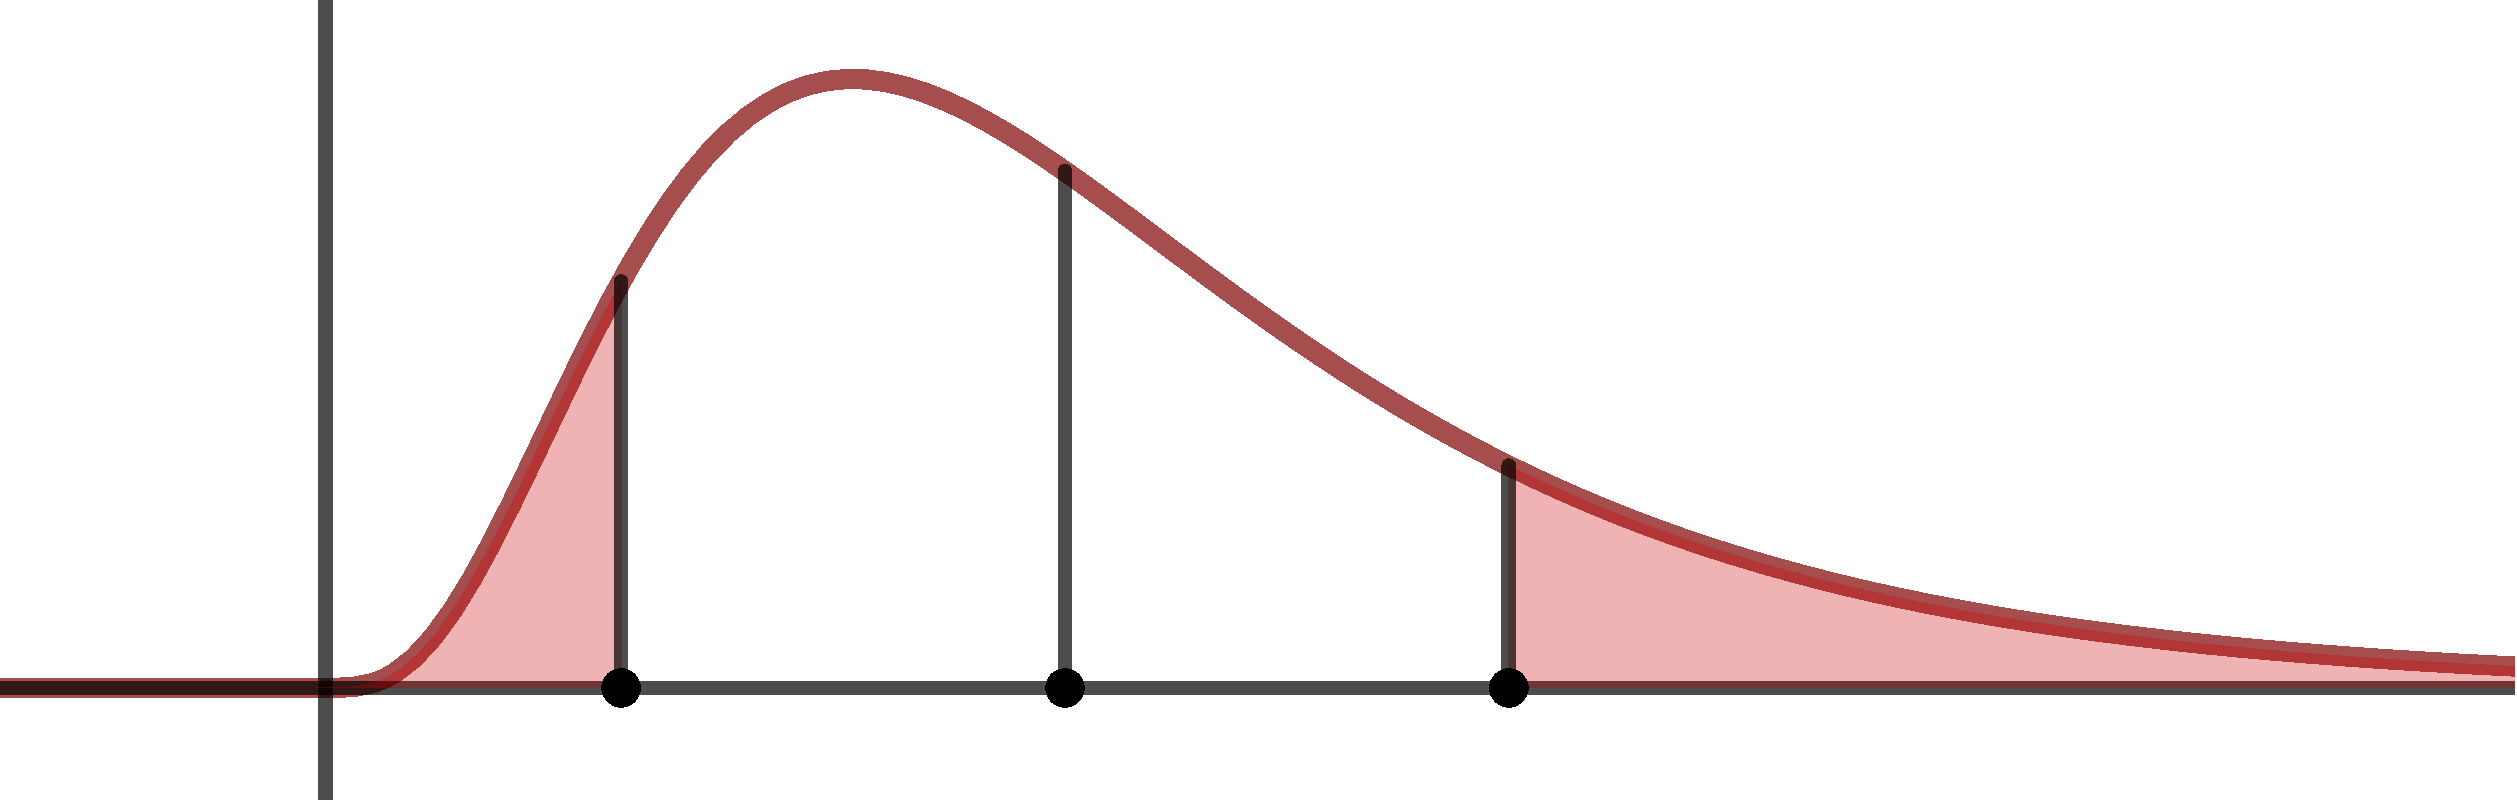
\includegraphics[width=10cm]{Images/FDistrib}};
	\draw [color=black](-3.1,-0.45) node[anchor=north west] {$\frac{\alpha}{2}$};
	\draw [color=black](1.0,-0.45) node[anchor=north west] {$\frac{\alpha}{2}$};
	\draw [color=red!20!black](0.35,1.00) node[anchor=north west] {Fisherova distribuce};
	\draw [color=red!40!black](0.7,0.50) node[anchor=north west] {$F_{12}\sim\FF(n_1-1,n_2-1)$};
	\draw [color=black](-4.2,-1.25) node[anchor=north west] {$0$};
	\draw [color=black](-2.9,-1.25) node[anchor=north west] {$K_L$};
	\draw [color=black](-1,-1.25) node[anchor=north west] {$1$};
	\draw [color=black](0.75,-1.25) node[anchor=north west] {$K_H$};
	\end{tikzpicture}
	\caption{Kritický obor F-testu homogenity rozptylů.}
	\label{fig:fisher}
\end{figure}
\begin{remark}
		V praxi lze použít testovací statistiku $$\widetilde{F}_{12}=\frac{\max(s_1^2,s_2^2)}{\min(s_1^2,s_2^2)}\sim \FF(n'-1,n''-1),\text{ kde }\quad \begin{array}{l}
	n'= \max(n_1,n_2),\\n''=\min(n_1,n_2),
	\end{array} $$ kterou pak porovnáváme pouze s~horním $\FF_{1-\frac{\alpha}{2}}$ příslušným kvantilem Fisherova rozdělení.
\end{remark}
\section{Test koeficientu korelace ($\mathcal{N}_2$)}
Předpokládejme $ (X_j,Y_j)_{j=1}^n ~iid~\NN_2(\mu_1,\mu_2,\sigma_1^2,\sigma_2^2,\rho)$ z~dvourozměrného nedegenerovaného Gaussova rozdělení při~$\sigma_1>0,~\sigma_2>0,~\abs{\rho}<1$. Testujeme nekorelovanost $X,Y$, tzn. nulovou hodnotu korelačního koeficientu $\rho=\rho(X,Y)$: $$H_0:\rho=0~\text{vs.}~H_1:\rho\neq 0\qquad(\text{tzn. test nezávislosti }X\text{ a~}Y\text{ v~}\NN_2\text{ modelu})$$ na~hladině významnosti $\alpha\in(0,1)$.\\
\textbf{Odvodíme LRT test} $H_0$:\\
Logaritmická věrohodnostní funkce modelu $\NN_2(\mu_1,\mu_2,\sigma_1^2,\sigma_2^2,\rho)$ při~označení $\t=(\mu_1,\mu_2,\sigma_1^2,\sigma_2^2,\rho)$ je 
\[
\begin{split}
&l(\t)=\ln L(\t)=\frac{-1}{2(1-\rho^2)}\Big[ \sum\limits_{j=1}^{n}\frac{(X_j-\mu_1)^2}{\sigma_1^2}+\sum\limits_{j=1}^{n}\frac{(Y_j-\mu_2)^2}{\sigma_2^2}-\\&-2\rho\sum\limits_{j=1}^{n}\frac{(X_j-\mu_1)(Y_j-\mu_2)}{\sigma_1\sigma_2}\Big] -n\ln\br{2\pi\sigma_1\sigma_2\sqrt{1-\rho^2}} . \end{split}
\]
Následně vyhodnotíme výraz
$$ \Lambda(\textbf{x},\textbf{y})=\frac{\sup\{ L(\t):\mu_1,\mu_2,\sigma_1^2,\sigma_2^2,\rho=0 \}}{\sup\{ L(\t):\mu_1,\mu_2,\sigma_1^2,\sigma_2^2,|\rho|<1\}}\sim \frac{\text{4 rovnice typu }\partial_r \ln L=0}{\text{5 rovnic typu }\partial_l\ln L=0}.$$
Řešením obou extrémů jsou MLE odhady: $\widehat{\mu}_1=\oxn$, $\widehat{\mu}_2=\oyn$, $\widehat{\sigma}_1^2=\widehat{\sigma}_{n,X}^2$ a~$\widehat{\sigma}_2^2=\widehat{\sigma}_{n,Y}^2$ a~dále
$$ \widehat{\rho}_{_{XY}}=\widehat{\rho}_{n}(\X,\Y)=\frac{\sum_{j=1}^n (X_j-\Oxn)(Y_j-\Oyn)}{\sqrt{\sum_{j=1}^n(X_j-\Oxn)^2\sum_{j=1}^n(Y_j-\Oyn)^2}}=\frac{\widehat{\Cov}_{XY}}{\widehat{\sigma}_1\cdot\widehat{\sigma}_2}, $$ který se~nazývá \textbf{Pearsonův výběrový koeficient korelace}. Dosazením těchto odhadů do~$\Lambda(\textbf{x},\textbf{y})$ získáme 
\[
\begin{split}
\ln\Lambda(\textbf{x},\textbf{y})&=\ln L(\widehat{\mu}_1,\widehat{\mu}_2,\widehat{\sigma}_1,\widehat{\sigma}_2,\rho=0)-\ln L(\widehat{\mu}_1,\widehat{\mu}_2,\widehat{\sigma}_1,\widehat{\sigma}_2,\widehat{\rho}_{XY})=\\&=-n\ln(2\pi\widehat{\sigma}_1\widehat{\sigma}_2)+n\ln\br{2\pi \widehat{\sigma}_1\widehat{\sigma}_2\sqrt{1-\widehat{\rho}_{XY}^2}}=\\&=\frac{n}{2}\ln\br{1-\widehat{\rho}_{XY}^2}\leq K~\Leftrightarrow~ \big| \widehat{\rho}_{XY} \big|\geq K'\Leftrightarrow~ \frac{|\widehat{\rho}_{XY}|\sqrt{n-2}}{\sqrt{1-\widehat{\rho}_{XY}^2}}\geq K'',
\end{split}
\]
kde $K,K',K''$ jsou vhodné konstanty nezávislé na~$(\textbf{x},\textbf{y})$. Lze ukázat, že při~platnosti $H_0:\rho=0$ má testovací LRT statistika rozdělení $$T=T(\X,\Y)=\frac{\widehat{\rho}_{_{XY}}\sqrt{n-2}}{\sqrt{1-\widehat{\rho}_{_{XY}}^2}}\sim t(n-2),$$ tedy Studentovo rozdělení s~$(n-2)$ stupni volnosti. To vede na~kritický obor testu $H_0:\rho=0$ ve~tvaru $$ W_\alpha=\left\{ (\textbf{x},\textbf{y}):\abs{T(\textbf{x},\textbf{y})}\geq t_{1-\frac{\alpha}{2}}(n-2) \right\}, $$ opět s~použitím $\Br{1-\frac{\alpha}{2}}$-kvantilu příslušného Studentova rozdělení.
\begin{example} Mějme následující dvourozměrná pozorování (data) o~rozsahu $n=10$
	$$	\begin{array}{c|cccccccccc}
	x_j & 94 & 98 & 127 & 88 & 85 & 95 & 111 & 75 & 102 & 82 \\ \hline
	y_j & 2.1 & 1.9 & 3.5 & 1.5 & 3.2 & 1.6 & 1.9 & 2.5 & 2.6 & 1.9
	\end{array} $$ pocházející z~náhodného výběru $(X_j,Y_j)_{j=1}^n~iid~\NN(\mu_1,\mu_2,\sigma_1^2,\sigma_2^2,\rho)$. Pro~test nekorelovanosti (zde i~test nezávislosti) $X$ a~$Y$ na~hladině $\alpha=0.05$ spočteme pro~$n=10$ následující hodnoty $$
	\widehat{\rho}_{X,Y}=0.3425,\quad T=\frac{\widehat{\rho}_{XY}\sqrt{n-2}}{\sqrt{1-\widehat{\rho}_{XY}^2}}=1.031,\quad
	t_{1-\alpha/2}(n-2)=t_{0.975}(8)=2.306.$$
	Nyní tedy testujeme $W_\alpha:~|T|\geq t_{0.975}(8)$? Nerovnost ale neplatí, a~proto $H_0$ nezamítáme na~hladině $\alpha=0.05$.
	Pokud síla testu $\beta$ (silofunkce) je dostatečně vysoká, např. $\beta>\beta_1$ na intervalu $\rho\in(-1,-\delta)\cup(\delta,1)$, pak $H_0$ přijímáme, tzn. s~danou signifikací $1-\beta_1$ deklarujeme, že mezi~Gaussovskými náhodnými veličinami $X$ a~$Y$ není korelační vztah, tedy $X$ a~$Y$ jsou nezávislé.
\end{example}

\chapter{Asymptotické testy hypotéz}

Doposud jsme pracovali převážně s~formou testů statistických hypotéz, které využívaly odvozené (UMP,UMPU,LRT) nebo jinak odůvodněné (RT) testovací statistiky $T_n=T_n(\X)$, pro~které bylo možné odvodit konkrétní \textbf{přesné} rozdělení $T_n\big|_{H_0}\sim\FF_{T_n}$ za~platnosti $H_0$ pro~daný fixní rozsah $n$ náhodného výběru $(X_j)_{j=1}^n$. K~tomu byla vyžadována specifická znalost statistického modelu, např. Gaussovskost pro~t-test, F-test, ANOVA,...

V mnoha případech však v~praxi, po~naměření nebo obdržení dat z~nějakého komplikovanějšího experimentu, narážíme na~dva problémy:
\begin{enumerate}[a)]
	\item Statistický model, ze~kterého pochází naše data, není znám (technologie měření není dostupná) nebo je znám pouze přibližně na~základě statistických testů shody dat s~předpoklá- daným rozdělením. Tyto testy však opět fungují pouze na~určité hladině spolehlivosti (signifikanci), jsou velmi často navíc založené pouze na~limitních větách, a~proto předpoklad statistického modelu pak může být zavádějící či dokonce chybný.
	\item Statistický model sice umíme více méně přesně odhalit, ale je nepříznivý v~tom smyslu, že pro~něj nedokážeme explicitně dovodit rozdělení vhodné testovací statistiky $T_n\big|_{H_0}$ pro~dané fixní $n$. To často nastává, pokud data pochází z~nestandardních distribucí nebo z~více-komponentních distribučních směsí.
\end{enumerate}

Obě tyto komplikace se~dají překonat, pokud máme k~dispozici střední či vyšší rozsahy $n$ souborů naměřených dat. To umožňuje aproximovat rozdělení vhodně zvolené testovací statistiky $T_n\big|_{H_0}$ limitním rozdělením při~$n\to+\infty$ ve~smyslu (slabé) limity v~distribuci, tzn. $T_n\big|_{H_0}\Dto \mathrm{G}$, kde limitní distribuční funkce $\mathrm{G}$ je nezávislá na~neznámých parametrech modelu. Aby se~toho dalo dosáhnout, je někdy potřeba nalézt navíc posloupnosti $(a_n)_{n=1}^{+\infty}\in\R$, $(b_n)_{n=1}^{+\infty}>0$, pro~které
$$ T_n'(\X)=\frac{T_n(\X)-a_n}{b_n}\bigg|_{H_0}\Dto \mathrm{G}\quad\Br{\text{tzn. }T_n'\sim\mathrm{A\mathrm{G}}(a_n,b_n^2)}. $$
Následně použijeme přibližné rozdělení $\mathrm{G}$ ke~konstrukci tzv. \textbf{asymptotického testu} $\crossedphi_\alpha$, resp. jeho příslušné kritické oblasti
$$ W_\alpha=\left\{ T_n(\textbf{x})\gtreqless K_\alpha \right\}\equal{\text{resp}.}\left\{ T_n'(\textbf{x})\gtreqless K_\alpha' \right\}\quad\text{tak, aby} $$
$$ \lim\limits_{n\to+\infty}\PP(\text{chyby I. druhu})=\lim\limits_{n\to+\infty}\PP(T_n(\X)\gtreqless K_\alpha)\equal{\text{resp}}\lim\limits_{n\to+\infty}\PP(T_n'(\X)\gtreqless K_\alpha' )=\alpha\quad\text{za platnosti }H_0. $$
K doladění konstanty $K_\alpha'$ opět použijeme vhodné typy kvantilů limitního rozdělení $\mathrm{G}$, například $\mathrm{G}_{1-\alpha},$ $\mathrm{G}_\alpha,$ $\mathrm{G}_{1-\frac{\alpha}{2}}$, podle povahy nerovností $\gtreqless$ charakterizující $W_\alpha$. Dosažené signifikanci testu $\alpha$ skrze toto limitní rozdělení $\mathrm{G}$ pak říkáme \textbf{asymptotická hladina} (\textit{size}) testu a~test založený na~takové $W_\alpha$ se~nazývá \textbf{asymptotický (přibližný) test} hypotézy $H_0$ vs. $H_1$.

\section{Asymptotické testy středních hodnot $iid~\LL_2$}
\begin{theorem}[Jednovýběrový asymptotický test $\mu=\mu_0$]
	Mějme náhodný výběr $X_1,...,X_n~iid~\LL_2$ pocházející z~libovolného rozdělení s~$\E X_j=\mu$ a~s~konečným rozptylem $\D X_j=\sigma^2>0$, který je neznámý. Testujeme hypotézu $\hypothesis{\mu=\mu_0}{\mu\neq\mu_0}$ (resp. $\mu\gtrless\mu_0$ apod.) na~hladině $\alpha\in(0,1)$. Pak testovací statistika
	$$ T_n=T_n(\X)=\sqrt{n}~\frac{\oxn-\mu_0}{s_n}\Dto \n{0,1} $$ za~platnosti $H_0$. Následně test $H_0:\mu=\mu_0$, založený na~kritické oblasti $W_\alpha=\left\{ \abs{T_n(\textbf{x})}\geq u_{1-\frac{\alpha}{2}} \right\}$, kde $u_{1-\frac{\alpha}{2}}$ značí kvantil $\n{0,1}$, zamítá $H_0$ na~\textbf{asymptotické hladině} $\alpha$.
	\begin{proof}
		Plyne triviálně z~asymptotických vlastností $\Oxn$ a~$s_n$ v~$\LL_2$, viz kapitola 1.
	\end{proof}
\end{theorem}
\begin{remark}
	Test je asymptotický a~tedy vyžaduje dostupnost dostatečně velkého počtu experimentálních dat $(x_j)_{j=1}^n$, avšak to je vyváženo tím, že statistický (apriorní) model pro~tyto realizace může být zcela neznámého typu, splňující~pouze předpoklad konečného $\sigma^2>0$.
\end{remark}
\begin{theorem}\label{veta52}
	Nechť $X$ a~$Y$ jsou nezávislé z~$\LL_2$ a~mějme dva náhodné výběry (např. testovací a~kontrolní) $(X_i)_{i=1}^{n_1}~iid~\LL_2(\mu_1,\sigma_1^2>0)$ a~ $(Y_j)_{j=1}^{n_2}~iid~\LL_2(\mu_2,\sigma_2^2>0)$. Pak 
	$$ T_{12}=T_{12}(\X,\Y)=\frac{\Ox{1}-\Oy{2}-(\mu_1-\mu_2)}{\sqrt{\frac{s_1^2}{n_1}+\frac{s_2^2}{n_2}}}\Dto \NN(0,1),\qquad\text{ při~}n_1,n_2\to+\infty. $$
	\begin{proof}[Schéma důkazu] Zavedeme
		$$ U_{n}=\sum\limits_{i=1}^{n_1}\underbrace{\frac{1}{n_1}\frac{X_i-\mu_1}{\sigma_{12}}}_{\xi_i}+\sum\limits_{j=1}^{n_2}\underbrace{\frac{-1}{n_2}\frac{Y_j-\mu_2}{\sigma_{12}}}_{\eta_j}=\sum\limits_{i=1}^{n_1}\xi_i+\sum\limits_{j=1}^{n_2}\eta_j, $$ kde $\sigma_{12}:=\sqrt{\frac{\sigma_1^2}{n_1}+\frac{\sigma_2^2}{n_2}}$ a~$n=n_1+n_2$. Nemůžeme použít standardní Lindeberg-Lévyho CLT, protože v~$U_{12}$ nemáme součty stejně rozdělených náhodných veličin. Přímým výpočtem však ověříme, že pro~$\forall i\in\widehat{n_1},~\forall j\in\widehat{n_2}$, platí\\
		 $\E\xi_i=0,\E\eta_j=0$ a~$\D\xi_i<+\infty,\D\eta_j<+\infty$, přičemž $B_n^2:=\sum\limits_{i=1}^{n_1}\D\xi_i+\sum\limits_{j=1}^{n_2}\D\eta_j=1$, kde jsme označili $n:=n_1+n_2$. Nyní budeme aplikovat obecnější CLT Lindeberg-Fellerův, tzn. je potřeba ověřit Lindebergovu podmínku $LP_n^\epsilon\to0,~\forall\epsilon>0$ (viz 01MIP):
		$$ LP_n^\epsilon=\sum\limits_{i=1}^{n_1}\E\big[ \xi_i^2 \Identita{|\xi_i|>\epsilon}\big] +\sum\limits_{j=1}^{n_2}\E\big[ \eta_j^2 \Identita{|\eta_j|>\epsilon} \big] \to0,\quad \forall\epsilon>0. $$ Následně z~CLT$_{L-F}$ postupně dostáváme 
		$$
		\overline{U}_{n}=\frac{1}{n}U_{n}\sim \AN\Br{\omn,\frac{\overbar{\rule{0ex}{1.2ex}\sigma_n}^2}{n}}=\AN\Br{0,\frac{1}{(n_1+n_2)^2}},\quad\text{tzn. }U_{n}\Dto\n{0,1}. $$
		Protože víme, že 
		$$ s_1^2\sj \sigma_1^2~\wedge~s_2^2\sj \sigma_2^2~~~\Rightarrow~~~ \sqrt{\frac{s_1^2}{n_1}+\frac{s_2^2}{n_2}}\sj \sqrt{\frac{\sigma_1^2}{n_1}+\frac{\sigma_2^2}{n_2}} ,$$
		dostaneme ze~Slutskyho lemmatu finální výsledek $T_{12}\Dto\n{0,1}$.
	\end{proof}
\end{theorem}

\begin{dusl}[Dvouvýběrový asymptotický test $\mu_1=\mu_2$]
	Díky větě \ref{veta52} lze zkonstruovat asymptotický test pro~testování hypotézy $H_0:\mu_1=\mu_2$ v~obecném $\LL_2$ modelu, kdy máme k~dispozici dva nezávislé náhodné výběry ze~dvou potenciálně zcela typově odlišných libovolných ditribucí $\FF_X$ a~$\FF_Y$, o~kterých víme pouze to, že obě distribuce mají konečné neznámé rozptyly $\sigma_1^2>0$, $\sigma_2^2>0$. Test $H_0:\mu_1=\mu_2$, založený na~kritické oblasti 
	$$ W_\alpha=\left\{ \abs{T_{12}(\textbf{x},\textbf{y})}\geq u_{1-\frac{\alpha}{2}} \right\},\quad\text{kde }T_{12}(\textbf{x},\textbf{y})=\frac{\overline{x_1}-\overline{y_2}}{\sqrt{\frac{s_1^2}{n_1}+\frac{s_2^2}{n_2}}}, $$
	zamítá $H_0$ na~asymptotické hladině $\alpha$. Hranice zamítnutí $u_{1-\frac{\alpha}{2}}$ zde opět označuje příslušný kvantil Gaussova rozdělení $\n{0,1}$.
	
\end{dusl}
\section{Asymptotický LRT a~Waldův test v~$\R^k$}
\begin{theorem}\label{veta55}
	Mějme $\t\in\Theta\subset\R^k$ a~testujeme hypotézu $\hypothesis{\t=\t_0}{\t\neq\t_0}$ na~základě náhodného výběru $X_1,...,X_n~iid~f\in\mathcal{F}$. Nechť jsou dále splněny předpoklady z~věty \ref{ANMLE}  o~asymptotické normalitě MLE odhadů, tedy $\mathcal{F}=\fregml$, a~nechť $\mathbb{I}(\t)$ je spojitá ($k\times k$ Fisherova informační matice) v~bodě $\t_0$. Pak za~platnosti $H_0$ platí
	$$ \lambda_n(\X)=-2\ln\Lambda(\X)\Dto \chi^2(k). $$ 
	\begin{proof}
		Provedeme důkaz pro~dimenzi $k=1$. Předpokládejme, že $H_0:\t=\t_0$ platí a~že $\widehat{\t}_n=\html$ je konzistentním řešením $LE_q$ z~věty \ref{ANMLE}  o~AN MLE odhadů. Pak Taylorem dostaneme 
	\[
	\begin{split}
	\lambda_n(\X)&=-2\ln\Lambda(\X)=-2\ln\frac{\sup\{ L(\t):\t=\t_0 \}}{\sup\{ L(\t):\t\in\Theta \}}=2\br{l(\widehat{\t}_n)-l(\t_0)}=\\&=
	2 l(\widehat{\t}_n)-2l(\widehat{\t}_n)-2(\t_0-\widehat{\t}_n)\underbrace{l'(\widehat{\t}_n)}_{0}-(\t_0-\widehat{\t}_n)^2 l''(\widehat{\t}_n)+\frac{1}{3}(\widehat{\t}_n-\t_0)^3 l'''(\t_n^\ast),
	\end{split}
	\] kde $\t_n^\ast\in\abs{\t_0,\widehat{\t}_n}$. Předchozí vztah upravíme na~
	$$ \lambda_n(\X)=\left\{ \sqrt{n}(\widehat{\t}_n-\t_0)\Big[ -\frac{1}{n}l''(\widehat{\t}_n) \Big]^{\frac{1}{2}} \right\}^2+\frac{1}{3}(\widehat{\t}_n-\t_0)\big[ \sqrt{n}(\widehat{\t}_n-\t_0) \big]^2\cdot\frac{1}{n}l'''(\t_n^\ast), $$
	\begin{tabular}{lll}
	kde & $\sqrt{n}(\widehat{\t}_n-\t_0)\Dto \n{0,\frac{1}{\fisher(\t_0)}}$, & (viz MLE $\htn$ věta  \ref{ANMLE}),\\
	 & $-\frac{1}{n}l''(\widehat{\t}_n)\Pto \fisher(\t_0)>0$, & (ze spojitosti $\fisher(\t)$ v~$\t_0$), \\
	  & $(\widehat{\t}_n-\t_0)\Pto 0$, & (z konzistence $\widehat{\t}_n$), \\
	  & $\big[ \sqrt{n}(\widehat{\t}_n-\t_0) \big]^2\Dto \Big[ \n{0,\frac{1}{\fisher(\t_0)}} \Big]^2$, & $\br{g(t)=t^2\text{ spojitá}}$, \\
	  & $\abs{\frac{1}{n}l'''(\t_n^\ast)}<M$ s~pravděpodobností jdoucí k~1 & (stejně jako ve~větě \ref{ANMLE} o~MLE).
	\end{tabular}
~\\~\\
Pak celkově ze~Slutskyho lemma dostáváme 
$$ \lambda_n(\X)\Dto\big[ \n{0,1} \big]^2=\chi^2(1). $$
	
	\end{proof}
\end{theorem}
\begin{dusl}[Asymptotický LRT]
	Za předpokladů věty \ref{veta55} je test hypotézy\\ $\hypothesis{\t=\t_0}{\t\neq\t_0}$, založený na~kritické oblasti 
	$$ W_\alpha=\Big\{ \textbf{x}:\lambda_n(\textbf{x})\geq \chi^2_{1-\alpha}(k) \Big\}, $$
	kde $\chi^2_{1-\alpha}(k)$ značí $(1-\alpha)$-kvantil příslušného $\chi^2(k)$ rozdělení, je tzv. \textbf{asymptotickým LRT testem}, který zamítá $H_0$ na~asymptotické hladině $\alpha$.
\end{dusl}
\begin{theorem}[Waldův test]
	Nechť $\t\in\Theta\subset\R^k$ a~testujeme $\hypothesis{\t=\t_0}{\t\neq\t_0}$ na~hladině $\alpha\in(0,1)$. Definujeme \textbf{Waldovu testovací statistiku} předpisem 
	$$ W_{\t_0}(\X)=n(\widehat{\t}_n-\t_0)^T\fisher(\t_0)(\widehat{\t}_n-\t_0), $$
	kde $\widehat{\t}_n$ je MLE. Pak při~stejných předpokladech jako ve~větě \ref{veta55} platí, že $W_{\t_0}(\X)\Dto \chi^2(k)$ za~platnosti $H_0$ a	\textbf{Waldův test} $H_0$, založený na~CR
	$$ W_\alpha=\Big\{ \textbf{x}: W_{\t_0}(\textbf{x})\geq \chi^2_{1-\alpha}(k) \Big\} $$ zamítá $H_0$ na~asymptotické hladině $\alpha$.
	\begin{proof}
		Důkaz ponechán čtenáři (triviální).
	\end{proof}
\end{theorem}
\begin{remark}
	Oba testy, asymptotický LRT i~Waldův test jsou konzistentní, tzn. jejich síla/silofunkce splňuje podmínku, že $$ \beta_{W_\alpha}(\t)\to1\text{ při~}n\to+\infty,\quad\forall\t\neq\t_0. $$
\end{remark}


\section{Testy dobré shody (GoF)}
Testy dobré shody jsou jedním z~velmi užitečných nástrojů při~identifikaci konkrétního typu statistického modelu, který stojí za~naměřenými realizacemi sledované náhodné veličiny (vlastnosti) $X$. Shoda těchto dostupných dat $\mathbf{x}=(x_i)_{i=1}^n$ s~apriorně předpokládaným modelem $F\in\mathcal{F}$ by měla být vždy ověřena ještě předtím než přistoupíme ke~statistickým testům nad~konkrétními parametry $\theta$ tohoto modelu. Tedy chceme-li po~provedeném experimentálním měření nějaké fyzikální či ekonomické veličiny $X$, začít testovat např. hypotézu $H_0: \ \mu=\mu_0$ prostřednictvím klasického $t$-testu, měli bychom nejdříve ověřit fakt, že experimentální data $\mathbf x$ skutečně mohou pocházet z~nějaké Gaussovské distribuce $\NN(\mu,\sigma^2)$ s~potenciálně neznámými parametry $\mu,\sigma^2>0$. Pokud se~takové potvrzení předpokládaného funkčního tvaru statistického modelu nezdaří, je potřeba buď prověřit kvalitu naměřených dat (přeměřit/doměřit data, upravit experiment) nebo přejít k~jinému vhodnějšímu statistickému modelu jiného typu využívající odlišný parametr $\widetilde{\theta}$ co do~jeho významu nebo dimenze. A~znovu testovat shodu dat s~tímto novým modelem.

Je patrné, že tato úloha prověření typu modelu je zcela zásadní a~rozhoduje o~kvalitě celého statistického šetření nebo predikce. Testy dobré shody jsou pouze jedním z~mnoha takových detekčních nástrojů pro~identifikaci relevantního statistického modelu, další možné přístupy viz 01MEX, 01SKE, a~jiné.

\begin{define}
	Mějme náhodnou veličinu (vlastnost) $X$ na~$(\Omega, \mathcal{A}, \mathbb{P})$ a~příslušný náhodný výběr $X_1,\ldots,X_n$ pocházející z~nějaké neznámé distribuce $\FF$. Volme jednu konkrétní distribuci $\FF_0\in \mathcal{F}$. Pak test hypotézy
	$$ H_0: \FF=\FF_0 \qquad vs. \qquad H_1: \FF\neq \FF_0 \text{ (resp. } \FF=\FF_1) $$
	se nazývá \textbf{testem dobré shody} (\textit{GoF - Goodness-of-Fit}) modelu $\FF_0$. Opět volíme hladinu významnosti $\alpha\in(0,1)$ a~testujeme $H_0$ na~této signifikantní hranici pro~chybu I.druhu. Tedy, za~kritickou chybu považujeme rozhodnutí o~zamítnutí modelu $\FF_0$, přestože ten je správný.
\end{define}

\subsection*{$\chi^2$-testy GoF}
Za jeden z~nejznámějších GoF testů lze považovat následující $\chi^2$-test, který převádí celou úlohu na~specifický {\em asymptotický} test v~Multinomickém parametrickém modelu za~cenu jistého \emph{binování} (diskretizace) dostupného náhodného výběru $\mathbf X$. Označme $H_X$ obor hodnot náhodné veličiny $X\sim \FF$ a~vytvořme dělení $\{A_1,\dots,A_k\}$ oboru hodnot $H_X$ na~$k$ disjunktních boxů či tříd (binů). Dále zavedeme
$$ p_j=\PP_\FF(X\in A_j), \qquad p_{0j}=\PP_{\FF_0}(X\in A_j), \qquad\forall j\in \widehat k.$$
Mějme nyní k~dispozici náhodný výběr $\mathbf X=(X_i)_{i=1}^n~iid~\FF$ a~nechť
$$ Y_j=\#\left\{i:\ X_i\in A_j\right\}= \sum_{i=1}^n \mathbb I\{X_i\in A_j\}= \sum_{i=1}^n \mathbb I_{A_j}(X_i)$$
je počet těch pozorování $X_i$ z~$\{X_1,\dots,X_n\}$, která se~vyskytují v~$j$-tém binu $A_j$, $j\in\widehat k$.
Vzhledem k~$iid$ předpokladu pro~jednotlivá $X_i$ pak plyne, že každé $Y_j \sim \mathrm{Bi}(n,p_j)$, a~proto i~celý vektor
$ \mathbf Y=(Y_1,\ldots,Y_k)$ má Multinomické rozdělení rozdělení $\mathbf Y \sim \mathrm{Mult}(n,\mathbf p)$, při~označení $\mathbf p=(p_1,\ldots,p_k)$.
Namísto testu $ H_0: \FF=\FF_0$ vs. $H_1: \FF\neq \FF_0$ pak testujeme parametrickou hypotézu na~hladině $\alpha>0$
$$ H_0: \mathbf p = \mathbf{p_0} \qquad\text{vs.}\qquad H_1: \mathbf p \neq \mathbf{p_0} \qquad\text{kde }\mathbf p_0= (p_{01},\ldots,p_{0k})$$
v Multinomickém modelu $\mathbf Y \sim \mathrm{Mult}(n,\mathbf p)$, přičemž $\sum_1^k p_j=\sum_1^k p_{0j}=1$.

\begin{theorem}\label{veta:Pearson3}
	Nechť $\widehat{p}_j=Y_j/n$ značí MLE odhady parametrů $p_j$ v~binomickém modelu $\mathrm{Bi}(n,p_j)$, $\forall j\in \widehat k$. Následující tři testovací statistiky v~$\mathrm{Mult}(n,\mathbf p)$ modelu
	\begin{align*}
	\chi^2(\mathbf Y) & = \sum_{j=1}^k \frac{n(\widehat{p}_j-p_{0j})^2}{p_{0j}}=  \sum_{j=1}^k \frac{(Y_j-np_{0j})^2}{np_{0j}} \qquad\text{(Pearsonova)}, \\
	\widetilde\chi^2(\mathbf Y) & = \sum_{j=1}^k \frac{n(\widehat{p}_j-p_{0j})^2}{\widehat{p}_j}= \sum_{j=1}^k \frac{(Y_j-np_{0j})^2}{Y_j} \qquad\text{(Neymanova)}, \\
	\lambda_n(\mathbf Y) & = -2\ln \Lambda(\mathbf Y)= -2\ln \prod_{j=1}^k \left(\frac{p_{0j}}{\widehat{p}_j}\right)^{n\widehat{p}_j} = -2 \sum_{j=1}^k Y_j \ln \left(\frac{np_{0j}}{Y_j}\right) \qquad\text{(LRT stat.)},
	\end{align*}
	jsou za~platnosti $H_0: \mathbf p=\mathbf p_0$ asymptoticky ekvivalentní a~všechny konvergují v~distribuci k~limitnímu $\chi^2(k-1)$ rozdělení.
\end{theorem}

\begin{proof}
	Protože platí $\sum_1^k p_j=\sum_1^k p_{0j}=1$, je skutečná dimenze testovaného parametrického prostoru $\Theta=\{(p_1,\ldots,p_k): p_j\in(0,1)\}$ rovna $k-1$. Pak z~věty \ref{veta55} o~asymptotickém LRT testu víme, že za~platnosti $H_0$ platí $ \lambda_n (\mathbf Y) \stackrel{\mathscr{D}}{\longrightarrow} \chi^2(k-1)$, protože jsou naplněny předpoklady na~ML-regularitu $\mathrm{Mult}(n,\mathbf p)$ systému. Dále lze ukázat pomocí Taylorova rozvoje funkce\\ $\ln (1+u)$ a~s využitím asymptotických vlastností MLE odhadů $\widehat{p}_j$, že\\ $\lambda_n(\mathbf Y)=\chi^2(\mathbf Y) + o_p(1)$. Pak ze~Slutskyho lemma mají $\lambda_n(\mathbf Y)$ a~$\chi^2(\mathbf Y)$ shodné asymptotické rozdělení. Podobně pro~$\widetilde\chi^2(\mathbf Y)$.
\end{proof}

\begin{dusl}[Pearson $\chi^2$ GoF]
	Test $H_0: \mathbf p = \mathbf p_0$ založený na~kritické oblasti
	$$ W_\alpha=\Big\{ \mathbf y: \chi^2(\mathbf y) \geqslant \chi^2_{1-\alpha}(k-1)\Big\} \qquad (\chi^2_{1-\alpha}\text{ značí kvantil }\chi^2\text{ rozdělení)}$$
	je asymptotickým Pearsonovým $\chi^2$-testem dobré shody dosahujícím asymptotické signifikance $\alpha$. Podobně pro~$\widetilde\chi^2(\mathbf Y)$ a~$\lambda_n(\mathbf Y)$ testovací statistiky.
\end{dusl}

Jde o~asymptotický test, tedy je vyžadován jednak dostatečný počet $n$ pozorování $(x_i)_1^n$, obvykle alespoň $n\geqslant 50$, a~současně by měla být splněna podmínka $np_{0j}\geqslant 5$, $\forall j\in\widehat k$. Hodnoty testovacích statistik $\chi^2(\mathbf y)$ a~$\widetilde\chi^2(\mathbf y)$ představují součet vážených kvadratických odchylek tzv.\ \emph{pozorovaných četností} $y_j$ od~\emph{teoretických četností} $np_{0j}$ přes všechny biny $A_j$, $j\in\widehat k$.

\subsection*{Kolmogorov-Smirnovův GoF test}
Test dobré shody dat s~modelem $ H_0: \FF=\FF_0$ vs. $H_1: \FF\neq \FF_0$ na~hladině $\alpha$ lze také provést čistě neparametrickým způsobem s~využitím empirické distribuční funkce $$\FF_n(t)=\FF_n(t,\mathbf X)=\frac{1}{n}\sum_{i=1}^n \mathbb{I}_{(-\infty,t]}(X_i),$$ jejíž statistické asymptotické vlastnosti byly uvedeny v~kapitole \ref{kapitola2}.

\begin{theorem}
	Nechť $\mathbf X=(X_i)_1^n$ jsou iid $\FF$ a~$\FF_n$ značí příslušnou empirickou distribuční funkci. Definujeme \textbf{Kolmogorov-Smirnovovu} statistiku
	$$ D_n(\FF)=\sup_{t\in\mathbb R}\big| \FF_n(t)-\FF(t) \big|= K(\FF_n,\FF) \quad\text{ (Kolmogorovova vzdálenost)}.$$
	Pak rozdělení $D_n(\FF)$ nezávisí na~modelu $\FF$, tzn.\ $D_n(\FF)$ je PQ pivotem pro~$\FF$. Dále $D_n(\FF)\sj 0$ a~asymptotické rozdělení $\sqrt{n}D_n(\FF)$ je dáno vztahem
	$$ \lim_{n\to+\infty} \mathbb P(\sqrt{n}D_n(\FF)\leq t)=1-2\sum_{m=1}^\infty (-1)^{m-1} e^{-2m^2t^2} =: G^{\txt{K\!S}}(t), \quad\forall t>0.$$
\end{theorem}

\begin{proof}
	Konvergence $D_n(\FF)\sj 0$ byla ukázána již v~kap.2 (Glivenko-Cantelli lemma).
	Asymptotické rozdělení $G^{\txt{K\!S}}$ ukázal Kolmogorov (1933). Za~DCv zbývá pouze prověřit fakt, že $D_n(\FF)$ je pivotální veličinou.
\end{proof}

\begin{dusl}[K-S GoF test]
	Test $H_0: \FF=\FF_0$ založený na~kritické oblasti
	$$ W_\alpha = \Big\{ \mathbf x: D_n(\FF_0)\geq K_\alpha\Big\} = \Big\{ \mathbf x: \sqrt{n}D_n(\FF_0)\geq K'_\alpha\Big\},$$
	kde $K'_\alpha=G_{1-\alpha}^{\txt{K\!S}}$ je $(1-\alpha)$-kvantil asymptotického Kolmogorov-Smirnovova rozdělení $G^{\txt{K\!S}}$, je testem $H_0$ na~asymptotické hladině $\alpha$. Tento test se~nazývá \emph{Kolmogorov-Smirnovův} (K-S) neparametrický test dobré shody.
\end{dusl}

Příslušné hodnoty kvantilů $G_{1-\alpha}^{\txt{K\!S}}$ limitního rozdělení $\sqrt{n}D_n(\FF_0)$, resp. $D_n(\FF_0)$, jsou tabelovány. Pro~jejich přibližný výpočet lze užít aproximaci $G^{\txt{K\!S}}(t)$ konečnou řadou. Použijeme-li takto pouze první člen řady pro~$m=1$, tzn.\ $G^{\txt{K\!S}}(t)\doteq 1-2 e^{-2t^2}$, dostaneme jednoduchý předpis pro~přibližnou hodnotu $(1-\alpha)$-kvantilu K-S rozdělení $K'_\alpha=G_{1-\alpha}^{\txt{K\!S}}\doteq \frac{\sqrt{2}}{2}[\ln 2-\ln \alpha]^{1/2}$.

%%%%%%%%%%%%%%%%%%%%%%%%%%%%%%%%%%%%%%%%%%%%%%%%%%%%%%%%%%%%%%%%%%%%%%%%%%%%%

\section{Modifikace $\chi^2$-testů dobré shody}
Pokud potřebujeme testovat shodu dat s~modelem ve~složené podobě, tzn.\
$$ H_0: \FF=\FF_\theta \quad vs. \quad H_1: \FF\neq \FF_\theta \qquad\text{ na~hladině }\alpha\in(0,1),$$
kde $\theta\in\Theta\subset\mathbb{R}^s$ je neznámý parametr takový, že $\mathrm{dim}(\Theta)=s$, pak postup testování upravíme následovně. Označíme opět
$$ p_j=\PP_\FF(X\in A_j), \qquad p_{0j}=p_{0j}(\theta)=\PP_{\FF_\theta}(X\in A_j), \quad\forall j\in \widehat k,$$
kde nyní $\mathbf p=(p_1,\ldots,p_k)$ a~$\mathbf p_0=\mathbf p_0(\theta) = \br{p_{01}(\theta),\ldots,p_{0k}(\theta)}$.
Na základě binovaných náhodných veličin $(Y_j)_{j=1}^k$ testujeme v~$\mathrm{Mult}(n,\mathbf p)$ modelu parametrickou hypotézu
$$ H_0: \mathbf p = \mathbf{p}_0(\theta) \quad\text{ vs. }\quad H_1: \mathbf p \neq \mathbf{p}_0(\theta) \qquad\text{na hladině }\alpha>0. $$
Protože však nyní vektor $\mathbf p_0$ je funkcí neznámého parametru $\theta$, musíme tento parametr odhadnout za~platnosti $H_0$. Takový vhodný odhad $\widehat\theta_n=\widehat\theta_n(\mathbf Y)$ by měl disponovat dostatečně dobrými asymptotickými vlastnostmi při~$n\to+\infty$. Dostupnou realizaci odhadu $\widehat\theta_n(\mathbf y)$ pak dosadíme do~funkce $\mathbf p_0(\theta)$ a~testujeme již jednoduchou bodovou hypotézu v~Multinomickém modelu na~hladině $\alpha$
$$ H_0: \mathbf p = \widehat{\mathbf p}_0 \quad\text{ vs. }\quad H_1: \mathbf p \neq \widehat{\mathbf p}_0,
\qquad\text{kde } \widehat{\mathbf p}_0=\widehat{\mathbf p}_0\br{\widehat\theta_n(\mathbf y)}.$$
Toto zanesení odhadu $\widehat\theta_n$ do~testované hypotézy $H_0$ však modifikuje asymptotické vlastnosti použitých testovacích statistik.

\begin{theorem}
	Mějme test $ H_0: \mathbf p = \widehat{\mathbf p}_0$ vs. $H_1: \mathbf p \neq \widehat{\mathbf p}_0$ za~výše uvedených podmínek, kdy $\mathrm{dim}(\Theta)=s$. Nechť $\widehat\theta_n$ značí maximálně věrohodný odhad $\html(\mathbf Y)$ za~platnosti $H_0$.
	%nebo, alternativně, tzv.\ \emph{minimum $\chi^2$ odhad} $$\widehat\theta_n= \argmin_\theta \sum_{j=1}^k \frac{(Y_j-np_{0j}(\theta))^2}{np_{0j}(\theta)}.$$
	Pak testovací statistika
	$$\chi^2(\mathbf Y) = \sum_{j=1}^k \frac{(Y_j-n\widehat p_{0j})^2}{n\widehat p_{0j}} \Dto \chi^2(k-s-1)$$
	a test založený na~kritické oblasti
	$$ W_\alpha=\Big\{ \mathbf y: \chi^2(\mathbf y) \geqslant \chi^2_{1-\alpha}(k-s-1)\Big\} \qquad (\chi^2_{1-\alpha}\text{ značí kvantil }\chi^2 \text{ rozdělení)}$$
	je Pearsonovým $\chi^2$-testem dobré shody dosahujícím asymptotické signifikance $\alpha$. Podobně pro~testovací statistiky $\widetilde\chi^2(\mathbf Y)$ a~$\lambda_n(\mathbf Y)$.
\end{theorem}

\begin{proof}
	Podobně jako u~věty \ref{veta:Pearson3} s~využitím asymptotiky (zobecněného) LRT testu (nedělali jsme).
\end{proof}

\begin{remark}
	Takto upraveným $\chi^2$-testem dobré shody tedy umíme otestovat například hypotézu $H_0$, zda naše data $\mathbf y$ mohou pocházet z~nějakého libovolného rozdělení ze~systému Gaussovských distribucí, tzn. hypotézu
	$$ H_0:  \FF \in \mathcal \FF = \{ \mathcal N(\mu, \sigma^2): \theta=(\mu,\sigma^2)\in \mathbb R \times \mathbb{R}^{+}\}.$$ Avšak pozor, dosazované MLE odhady $\widehat \mu_n,\widehat\sigma_n^2$ nejsou běžné MLE odhady parametrů $\mu,\sigma^2$ vytvořené na~základě původně naměřených dat $(x_i)_1^n$, ale na~základě výhradně binovaných dat $(y_j)_1^k$ podléhajících Multinomickému modelu $\mathrm{Mult}(n,\mathbf p_0(\mu, \sigma^2))$. Obecně nesprávný, ale přesto užívaný postup testování normality dat $H_0: \FF=\NN(\mu,\sigma^2)$ je ten, kdy na~základě původních dat $(x_i)_1^n$ jsou spočteny standardní MLE odhady $\widehat\mu=\overline{x}_n$ a~$s_n^2=\sum_1^n(x_i-\overline{x}_n)^2/(n-1)$, poté je náhodný výběr $(X_i)_1^n$ tzv.\ 'standardizován' na~$U_i = (X_i-\overline{x}_n)/ s_n $ a~nakonec je testována hypotéza $H_0: \FF_U= \mathcal N(0,1)$ na~hladině $\alpha$ pomocí běžné Pearsonovy testovací statistiky aplikované na~'standardizovaná' data $(u_i)_1^n$.
\end{remark}



\chapter{Konfidenční množiny, Intervaly spolehlivosti}
Bodové odhady $\widehat{\t}_n(\X)=\widehat{\t}_n$, resp. $T_n(\X)=T_n$, sice poskytují odhad hodnoty daného parametru, nicméně například ve~spojitém statistickém modelu (ASR$_\lambda$) vždy platí, že\\ $\PP\br{\htn(\X)=\t_0}=0,~\forall\t_0$, resp. $\PP\br{T_n(\X)=\tau(\t)}=0,~\forall\t\in\Theta$. Z~tohoto důvodu se~zavádí tzv. interval spolehlivosti, což je interval, ve~kterém se~neznámý parametr $\t$ nachází s~námi zadanou pravděpodobností (například 95\%). Přesnost takového odhadu je pak dán šířkou tohoto intervalu.


\begin{define}
	Nechť $\X=(X_1,...,X_n)\sim\PP\in\mathscr{P}$ na~$(\Omega,\mathcal{A})$, označme $\theta=\theta(\PP)\in\Theta\subset\R^1$ funkcionál na~$\mathscr{P}$, resp. $\theta\in\Theta\subset\R^k$. Označíme $\Bb_\Theta$ systém borelovských podmnožin $\Theta$ a~zvolíme číslo $\alpha\in(0,1)$. Pak $C(\X)\in\Bb_\Theta$ se~nazývá \textbf{konfidenční množina} ($\mathrm{CM}_{1-\alpha}$) pro~$\theta$ na~hladině $(1-\alpha)$, pokud  $$\inf\limits_{\PP\in\mathscr{P}}\PP\br{\theta\in C(\X)}\geq 1-\alpha.$$ Číslo $\inf\limits_{\PP\in\mathscr{P}}\PP\br{\theta\in C(\X)}$ se~pak nazývá \textbf{konfidenční koeficient} (koeficient spolehlivosti).
	Pokud speciálně $C(\X)=\big[ \underline{\theta}(\X),\overline{\theta}(\X) \big]\subset\Theta$, nazveme ji \textbf{konfidenční interval} $(\mathrm{CI}_{1-\alpha})$ (interval spolehlivosti) na~hladině $1-\alpha$.
\end{define}
\begin{remark}
	$C(\X)$ je tedy "náhodná"~množina (založená na~náhodném výběru $\X$)\\ \textbf{pokrývající} skutečnou hodnotu parametru $\theta$ s~pravděpodobností alespoň $1-\alpha$, ať je tento skutečný neznámý parametr $\t$ kdekoliv ve~svém parametrickém prostoru $\Theta$. 
	
	Označíme-li
	$\EE{\lambda\br{C(\X)}}$ jako střední $\lambda$-objem konfidenční množiny, resp. střední $\lambda$-délku intervalu spolehlivosti, pak hledáme takovou $C(\X)$, která minimalizuje $\EE{\lambda\br{C(\X)}}$ stejnoměrně na~$\Theta$ při~podmínce, že konfidenční koeficient $\geq 1-\alpha$. Tato optimalizační úloha je však často neřešitelná, proto se~v~praxi většinou snažíme naplnit alespoň kritérium kladené na~konfidenční koeficient a~přitom dosáhnout rozumného objemu/délky $\lambda\br{C(\textbf{x})}$. Při~náhodném opakování celého experimentu pak víme, že $\mathrm{CM}_{1-\alpha}$ pokrývá skutečnou hodnotu parametru $\t$ v~průměru ve~$(1-\alpha)\cdot 100$\% případů. 
\end{remark}	


\section{Konstukce $\mathrm{CM}_{1-\alpha}$ pomocí pivotů (PQ)}\label{pivoty}
\begin{define}
	Borelovsky měřitelná funkce $\mathcal{R}(\X,\t)$ se~nazývá pivotální veličina (\textit{pivot}) (PQ) pro~parametr $\t$, pokud \textbf{rozdělení} $\mathcal{R}(\X,\t)$ nezávisí na~volbě $\PP\in\mathscr{P}$.
\end{define}

\subsection*{Metoda konstrukce $\mathrm{CM}_{1-\alpha}$ pro~$\t$:}
	\begin{enumerate}[1)]
		\item Nalezneme vhodnou \textbf{pivotální veličinu}  $\mathcal{R}(\X,\theta)$, pokud taková existuje. 
		\item Volíme pevně $\PP\in\mathscr{P}$ a~najdeme konstanty $c_1,c_2$ takové, že platí 
	$$ \PP\br{c_1\leq \mathcal{R}(\X,\theta)\leq c_2}\geq 1-\alpha,\quad \text{případně}\quad\PP\br{c_1\leq \mathcal{R}(\X,\theta)\leq c_2}=1-\alpha. $$ 
	\item Pak $C(\X)=\Big\{ \theta\in\Theta:~c_1\leq \mathcal{R}(\X,\theta)\leq c_2 \Big\}$ je $\mathrm{CM}_{1-\alpha}$.
	\begin{proof}
		Zřejmý.
	\end{proof}
	\end{enumerate}

Problémy konstrukce $C(\X)$:\begin{enumerate}[a)]
	\item existence alespoň jednoho pivotu $\mathcal{R}(\X,\t)$,
	\item existence mnoha různých $\mathcal{R}(\X,\t)$: tedy nevíme, kterou z~nich v~konstrukci $C(\X)$ použít, tzn. která poskytuje nejmenší střední objem/délku $C(\X)$,
	\item volba $c_1,c_2$: kritériem může být například  $\alpha/2$-symetrie, tzn. volba $c_1,c_2$ tak, aby\\ $\PP\br{\mathcal{R}(\X,\t)>c_2}=\frac{\alpha}{2}$ a~$\PP\br{\mathcal{R}(\X,\t)<c_1}=\frac{\alpha}{2}$.
	\item výpočet $C(\X)$ ze~soustavy nerovnic $c_1\leq \mathcal{R}(\X,\t)\leq c_2$: pokud je $\mathcal{R}(\X,\t)$ např. ryze rostoucí v~proměnné $\theta\in\R^1$, pak $C(\X)=\Big\{\t: \inv{\mathcal{R}}(c_1,\X)\leq \theta\leq \inv{\mathcal{R}}(c_2,\X) \Big\} $. Podobně pro~funkci $\mathcal{R}(\X,\t)$ regulární a~prostou vzhledem k~$\t\in\R^k$.
\end{enumerate}



\begin{example}\label{priklad}
	Mějme Gaussovský náhodný výběr $X_1,...,X_n~iid~\n{\mu,\sigma^2}$. \begin{enumerate}[a)]
		\item Chceme najít $\mathrm{CI}_{1-\alpha}$ pro~parametr $\t=\mu$, přičemž předpokládáme, že $\sigma^2$ neznáme. Víme, že t-statistika 
		$$ T(\X)=\frac{\sqrt{n}(\oxn-\mu)}{s_n}\sim t(n-1)\qquad(\text{Studentovo rozdělení}) $$
		a tedy $T(\X)$ je pivotální veličina pro~parametr $\mu$. Volme konstanty $c_1,c_2$ z~podmínky $\alpha/2$-symetrie následovně 
		$$ \PP\br{\underbrace{t_{\frac{\alpha}{2}}(n-1)}_{c_1}\leq T(\X)\leq \underbrace{t_{1-\frac{\alpha}{2}}(n-1)}_{c_2}}=1-\alpha. $$
		Ze soustavy nerovnic $t_{\frac{\alpha}{2}}\leq T(\X)\leq t_{1-\frac{\alpha}{2}}$ po~dosazení za~$T(\X)$ vyjádříme $\mu$, tzn. dostáváme $\mathrm{CI}_{1-\alpha}$ pro~$\mu$ v~Gaussovském modelu:
		$$ C(\X)=\left[ \Oxn-t_{1-\frac{\alpha}{2}}(n-1)\frac{s_n}{\sqrt{n}},\quad \Oxn+ t_{1-\frac{\alpha}{2}}(n-1)\frac{s_n}{\sqrt{n}} \right], $$ kde jsme použili vlastnost symetrie kvantilů $t_{\frac{\alpha}{2}}=-t_{1-\frac{\alpha}{2}}$ Studentova rozdělení. V~praxi se~někdy (nesprávně) tento $\mathrm{CI}_{1-\alpha}$ zapisuje jako 
		$$ \mu=\Oxn\pm t_{1-\frac{\alpha}{2}}(n-1)\frac{s_n}{\sqrt{n}}. $$
		\item Podobně lze získat $\mathrm{CI}_{1-\alpha}$ pro~parametr $\sigma^2$ při~neznámém $\mu$ prostřednictvím $\chi^2$-statistiky (PQ pro~$\sigma^2$):
		$$ \chi^2(\X)=\frac{(n-1)s_n^2}{\sigma^2}\sim\chi^2(n-1)\qquad(\text{Pearsonovo }\chi^2\text{-rozdělení}). $$
		Protože zde $\chi^2(n-1)$ není symetrické rozdělení, nelze $\mathrm{CI}_{1-\alpha}$ psát ve~tvaru $\sigma^2=\pm c_{\alpha,n}s_n^2$ ani $\sigma^2=s_n^2\pm c_{\alpha,n}$.
	\end{enumerate}
\end{example}

\begin{example}[Simultální $\mathrm{CM}_{1-\alpha}$ pro~$\NN$]
Mějme $\poslkon~iid~\NN(\mu,\sigma^2)$ a~uvažujme dvourozměrný parametr $\theta=(\mu,\sigma^2)$. Volme dvourozměrnou pivotální veličinu,\\ $\mathcal{R}(\X,\t)=\br{U(\X),\chi^2(\X)}$, kde \[
\begin{split}
U(\X)&= \sqrt{n}\frac{(\Oxn-\mu)}{\sigma}\sim\NN(0,1)\quad (PQ\text{ pro~}\mu\text{ při~fixním }\sigma^2), \\
\chi^2(\X)&=\frac{(n-1)s_n^2}{\sigma^2}\sim\chi^2(n-1)\quad (PQ\text{ pro~}\sigma^2\text{ nezávisle na~}\mu).
\end{split}
\]
Volíme konstanty $c_1,c_2$ tak, aby $\p{c_1\leq U(\X)\leq c_2}=\sqrt{1-\alpha}$, tzn. např. $c_1=-u_{1-\frac{\alpha}{2}}$ a~$c_2=u_{1-\frac{\alpha}{2}}$ kvantily $\n{0,1}$. Dále volíme konstanty $d_1,d_2$ tak, aby $\p{d_1\leq \chi^2(\X)\leq d_2}=\sqrt{1-\alpha}$, tzn. např. $d_1=\chi^2_{\frac{\alpha}{2}}(n-1)$ a~$d_2=\chi^2_{1-\frac{\alpha}{2}}(n-1)$ kvantily rozdělení $\chi^2(n-1)$. Ze~soustavy nerovností $\Big\{ c_1\leq U(\X)\leq c_2 \wedge d_1\leq\chi^2(\X)\leq d_2 \Big\}$ pak vyjádříme dvourozměrnou konfidenční množinu pro~$\t=(\mu,\sigma^2)$
$$ C(\X)=\left\{ (\mu,\sigma^2)\in\R\times\R^+:~\frac{n(\oxn-\mu)^2}{u^2_{1-\frac{\alpha}{2}}}\leq \sigma^2,~\frac{(n-1)s_n^2}{\chi^2_{1-\frac{\alpha}{2}}(n-1)}\leq \sigma^2\leq \frac{(n-1)s_n^2}{\chi^2_{\frac{\alpha}{2}}(n-1)} \right\}, $$
která dosahuje konfidenčního koeficientu přesně na~hladině $1-\alpha$. (nakreslete $C(\X)\subset\R\times\R^+$ za~DCv).
\end{example}

\section{Konstrukce $\mathrm{CM}_{1-\alpha}$ pomocí TSH $\crossedphi_\alpha$}\label{TSHkonst}
\begin{define}
	Nechť $\crossedphi(\textbf{x})$ je test hypotézy $H_0$ vs. $H_1$. Pak množinu $A(H_0)=\{ \textbf{x}:\crossedphi(\textbf{x})<1 \}$ nazýváme \textbf{přípustná oblast testu} $\crossedphi$ (ozn. AR - acceptance region). Speciálně pro~test $H_0:\t=\t_0$ označíme přípustnou oblast AR jako $A(\t_0)$.
\end{define}
\begin{remark}
	Nechť je test $\crossedphi$ pro~$H_0:\t=\t_0$ \textbf{neznáhodněný} a~tedy je charakterizován pro~dané $\t_0$ příslušnou kritickou oblastí typu $$W_\alpha=\left\{ T(\textbf{x})\leq K_1 \vee T(\textbf{x})\geq K_2 \right\}=\left\{ T(\textbf{x})\leq K_1 \right\}\cup\left\{ T(\textbf{x})\geq K_2 \right\}\equal{\text{ozn}}W_L\cup W_U$$
	na hladině testu $\alpha$, tzn. $\PP_{\t_0}(\X\in W_\alpha)=\PP_{\t_0}(\X\in W_L)+\PP_{\t_0}(\X\in W_U)=\alpha$. V~tomto případě pak platí, že $A(\t_0)=\left\{ \textbf{x}:T(\textbf{x})\in(K_1,K_2) \right\}=W_\alpha^c$, kde $\PP\br{\X\in A(\t_0)}=1-\alpha$. Tuto situaci ilustruje obrázek \ref{obrazek}.
\begin{figure}[h]
	\centering
	\begin{tikzpicture}
	\node[inner sep=0pt] (pic) at (0,0)
	{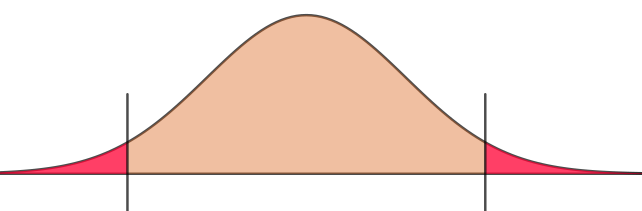
\includegraphics[width=6cm]{Images/acceptance_region}};
	\draw [color=black](-0.7,.3) node[anchor=north west] {$1-\alpha$};
	\draw [color=black](0.6,1.) node[anchor=north west] {$f_T\big|_{H_0}$};
	\draw [color=red!40!black](-2.95,-0.6) node[anchor=north west] {$W_L$};
	\draw [color=red!40!black](1.7,-0.6) node[anchor=north west] {$W_U$};
	\draw [color=red!40!black](-2.8,0.2) node[anchor=north west] {$\frac{\alpha}{2}$};
	\draw [color=red!40!black](1.7,0.2) node[anchor=north west] {$\frac{\alpha}{2}$};
	\draw [color=red!40!black](3.0,0.2) node[anchor=north west] {$W_\alpha=W_L\cup W_U$};
	\draw [color=black](-1.8,-0.7) node[anchor=north west] {Acceptance region};
	\draw [color=black](-0.7,-1.1) node[anchor=north west] {$A(\t_0)$};
	\end{tikzpicture}
	\caption{Souvislost $\mathrm{CI}_{1-\alpha}$ a~testování hypotézy $H_0:\t=\t_0$ skrze CR $W_\alpha$.}
	\label{obrazek}
\end{figure}
\end{remark}

Mějme  nyní náš statistický model $\PP\in\mathscr{P}$, parametr zájmu $\t=\t(\PP)$ a~náhodný výběr $X_1,...,X_n~iid~\PP_{\t}$.
\subsection*{Metoda konstrukce $\mathrm{CM}_{1-\alpha}$ pro~$\t$:}
\begin{enumerate}[1.]
	\item Volíme $\t_0\in\Theta$ libovolně pevně.
	\item Testujeme $H_0:\t=\t_0$ na~hladině významnosti $\alpha$. Příslušný test označíme $\crossedphi_\alpha$, resp. $W_\alpha$ pro~případ neznáhodněného testu.
	\item Vyjádříme $A(\t_0)$ pro~test $\crossedphi_\alpha$, resp. $W_\alpha$, při~libovolném $\t_0\in\Theta$. Tím získáme $A(\t)$ pro~$\forall\t\in\Theta$.
	\item Pak $C(\X)=\left\{ \t\in\Theta:\X\in A(\t) \right\}$ je $\mathrm{CM}_{1-\alpha}$ pro~$\t$. Navíc, pokud je test $\crossedphi_\alpha$ neznáhodněný a~je na~hladině $\alpha$, $\beta_{\crossedphi_\alpha}(\t_0)=\alpha$ pro~$\forall\t_0\in\Theta$, pak uvedená $C(\X)$ je $\mathrm{CM}_{1-\alpha}$ s~\textbf{konfidenčním koeficientem} rovným $(1-\alpha)$.
	\begin{proof}
		Ukážeme tvrzení z~bodu 4 pro~případ identifikovatelné rodiny $\mathscr{P}=\{\PP_\t\}$, ve~které je $\t$ jediným parametrem modelu (nejsou zde tzv. rušivé parametry):\[
		\begin{split}
		\inf\limits_{\PP\in\mathscr{P}}\PP\br{\t\in C(\X)}&=\inf\limits_{\t\in\Theta} \PP_{\t}\br{\t\in C(\X)}=\inf\limits_{\t\in\Theta} \PP_\t\br{\X\in A(\t)}=1-\sup\limits_{\t\in\Theta} \PP_\t\br{\X\notin A(\t)}=\\&=1-\underbrace{\sup\limits_{\t\in\Theta} \PP_\t\br{\crossedphi_\alpha(\X,\t)=1}}_{\leq\alpha}\geq 1-\alpha.
		\end{split}
		\]
	\end{proof}
\end{enumerate}
\begin{remark}
	Pokud $C(\X)$ vznikne prostřednictvím \textbf{neznáhodněného} UMP testu $\crossedphi_\alpha$ na~hladině $\alpha$ pro~$\forall\t_0\in\Theta$, pak $C(\X)$ nazveme UMA (\textit{uniformly most accurate}) $\mathrm{CM}_{1-\alpha}$ pro~$\t$. Podobně použitím $\txt{UMPU}$ testu na~hladině $\alpha$ získáme UMAU$_{1-\alpha}$ (\textit{UMA Unbiased, CM$_{1-\alpha}$}) pro~$\t$.
\end{remark}
\begin{example}
	Uvažujme statistický model $X_1,...,X_n~iid~\n{\mu,\sigma^2}$, kde $\sigma^2>0$ je neznámé. Jde nám o~$\mathrm{CI}_{1-\alpha}$ pro~parametr $\t=\mu$ na~hladině $\alpha\in(0,1)$. Testujeme pro~$\forall\mu_0\in\R$ hypotézu
	$$\hypothesiswide{\mu=\mu_0}{\mu\neq\mu_0}\quad\text{ na~hladině }\alpha.$$
	Použijeme LRT$_\alpha$ test s~příslušnou LRT kritickou oblastí
	$$ W_\alpha=\bigg\{ \textbf{x}:\abs{\frac{\sqrt{n}(\oxnn-\mu_0)}{s_n}}\geq \underbrace{t_{1-\frac{\alpha}{2}}(n-1)}_{K_\alpha} \bigg\},\quad\text{pro }\forall\mu_0\in\R. $$ Pak přípustná oblast pro~$\forall\mu_0\in\R$ je rovna 
	$$ A(\mu_0)=W_\alpha^c=\left\{ \textbf{x}:\abs{\frac{\sqrt{n}(\oxnn-\mu_0)}{s_n}}<t_{1-\frac{\alpha}{2}}(n-1) \right\} $$ nezávisle na~neznámém (rušivém) parametru $\sigma^2>0$. Pak podle bodu 4 konstrukce,
	$$ C(\X)=\left\{ \mu\in\R:\X\in A(\mu) \right\}=\abs{\begin{array}{l}
	\text{řešení příslušné}	\\ \text{nerovnosti v~}A(\mu) 
		\end{array} }=\Br{\Oxn-t_{1-\frac{\alpha}{2}}(n-1)\frac{s_n}{\sqrt{n}},\Oxn+t_{1-\frac{\alpha}{2}}(n-1)\frac{s_n}{\sqrt{n}}} $$
	je CI pro~$\mu$ s~konfidenčním koeficientem rovným $1-\alpha$. Tento CI je shodný s~CI$_{1-\alpha}$ získaným v~příkladu \ref{priklad} prostřednictvím pivotální náhodné veličiny $T(\X)$ (t-statistika).
\end{example}
\begin{remark}
	Všimněte si, že v~obou konstrukcích CM$_{1-\alpha}$ pomocí PQ pivotů nebo $\crossedphi_\alpha$ testů jsme neřešili velikost středního objemu/délky tohoto $C(\X)$, tzn. stejnoměrnou minimalizaci $\EE{\lambda\br{C(\X)}}$. Většinou je to úloha obtížná, mnohdy (explicitně) neřešitelná, na~stejné úrovni jako je úloha nalezení testu $\crossedphi_\alpha$ se~stejnoměrně maximální silofunkcí (silou) testu $\beta_{\crossedphi_\alpha}\big|_{H_1}$.
\end{remark}
\section{Asymptotické konfidenční množiny}
\begin{define}
	Mějme $\PP\in\mathscr{P}$ na~$(\Omega,\Aa),~\t=\t(\PP)\in\Theta\subset \R^1$, resp. $\Theta\subset\R^k$ a~$\Bb_\Theta$ Borelovské. Mějme $X_1,...,X_n\sim\PP\in\mathscr{P}$ a~$\alpha\in(0,1)$. Pak $C(\X)\in\Bb_\Theta$ se~nazývá \textbf{asymptotická} CM$_{1-\alpha}$, ozn ACM$_{1-\alpha}$, pokud pro
	$$\forall\PP\in\mathscr{P},\quad \lim\limits_{n\to+\infty}\PP\br{\t\in C(\X)}\geq 1-\alpha.$$
\end{define}
\subsection*{Metody konstrukce:}
\begin{enumerate}[I)]
	\item Najdeme takovou vhodnou náhodnou veličinu $\mathcal{R}_n(\X,\t)$, která je \textbf{asymptoticky pivotální} veličinou (ozn. APQ), tzn. její \textit{limitní} rozdělení nezávisí na~$\PP\in\mathscr{P}$: 
	$$\mathcal{R}_n(\X,\t)\Dto G,\quad\text{kde }G\text{ nezávisí na~}\PP\in\mathscr{P}.$$ 
	Toto limitní $G$ použijeme pro~konstrukci ACM$_{1-\alpha}$ stejně jako v~případě neasymptotických CM$_{1-\alpha}$ (viz sekce \ref{pivoty}).
	\item Stejně jako v~sekci \ref{TSHkonst}, pro~konstrukci ACM$_{1-\alpha}$ použijeme přípustnou oblast $A(\t_0)$ založenou na~asymptotickém testu $\crossedphi_\alpha$ dosahujícím asymptotické hladiny $\alpha$ pro~testování $H_0:\t=\t_0$. Tedy $C(\X)=\left\{ \t\in\Theta:\X\in A(\t)\right\}$, kde $A(\t)$ je AR asymptotického testu $\crossedphi_\alpha$, je ACM$_{1-\alpha}$ pro~parametr $\t$.  
\end{enumerate}
\begin{example}[I]
	Mějme $X\sim\FF\in\mathcal{F}$ a~volme $\t=\t(\FF)=\FF(t)$ pro~nějaké fixní $t\in\R$. Najdeme ACI$_{1-\alpha}$ pro~$\FF(t)$ založený na~$X_1,...,X_n~iid~\FF$ náhodného výběru. Víme, že $$\FF_n(t)=\frac{1}{n}\sumjn \Identita{(-\infty,t]}(X_j)\quad\text{(empirická c.d.f.)}$$ je náhodnou veličinou, která je $\AN$ odhadem $\FF(t)$ pro~$\forall t\in\R$, konkrétně\\ $\FF_n(t)\sim\AN\Br{\FF(t),\frac{1}{n}\FF(t)\br{1-\FF(t)}}$. Pak 
	$$ \mathcal{R}_n(\X)=\frac{\sqrt{n}\br{\FF_n(t)-\FF(t)}}{\sqrt{\FF(t)\br{1-\FF(t)}}}\Dto U\sim\n{0,1}, $$ a~proto $\mathcal{R}_n(\X)$ je APQ veličinou. Volíme $c_2=-c_1=u_{1-\frac{\alpha}{2}}$ kvantil $\n{0,1}$, pro který platí, že
	$$ \lim\limits_{n\to+\infty}\PP_\FF\br{\abs{\mathcal{R}_n(\X)}\leq u_{1-\frac{\alpha}{2}}}= \PP_{\n{0,1}}\br{\abs{U}\leq u_{1-\frac{\alpha}{2}}}=1-\alpha. $$
			Vyřešením nerovnosti $\abs{\mathcal{R}_n(\X)}\leq u_{1-\frac{\alpha}{2}}$ vzhledem k~$\FF(t)$ pak snadno dostaneme ACI$_{1-\alpha}$ pro~$\FF(t)$ při~fixním $t\in\R$.
\end{example}
\begin{example}[II]
	Mějme opět systém distribucí $\mathscr{P}$, $\t=\t(\PP)\in\Theta\subset\R^k$ a~$X_1,...,X_n~iid~\PP\in\mathscr{P}$. Pro~konstrukci ACM$_{1-\alpha}$ využijeme \textbf{asymptotický LRT} test $\hypothesis{\t=\t_0}{\t\neq\t_0}$ na~hladině $\alpha$ pro $\forall\t_0\in\Theta$. Víme, že za~platnosti $H_0$ a~předpokladu věty 5. má veličina $\lambda_n(\X)=-2\ln\Lambda(\textbf{x})$ asymptotické rozdělení $\chi^2(k)$, tzn. 
	$$ \lambda_n(\X)=-2\ln\frac{L(\t_0)}{L(\htn)}=2\br{l(\htn)-l(\t_0)}\Dto \chi^2(k)\quad \text{pro~}\forall\t_0\in\Theta, $$  kde $\htn$ je MLE odhad parametru $\t$. Příslušná LRT kritická oblast $W_\alpha=\left\{ \textbf{x}:\Lambda(\textbf{x})\leq K_\alpha \right\}$ vede na přípustnou oblast
	$$A(\t_0)=\left\{ \textbf{x}:\lambda_n(\textbf{x})<-2\ln K_\alpha\equal{\text{ozn}}K_\alpha' \right\}\quad \text{pro~}\forall\t_0,$$ pro~kterou však platí limitní vztah
	$$ \lim\limits_{n\to+\infty} \PP_{\t_0}\br{\X\in A(\t_0)}=\lim\limits_{n\to+\infty} \PP_{\t_0}\big( \underbrace{\lambda_n(\X)}_{\Dto\chi^2(k)}<\chi^2_{1-\alpha}(k) \big)=1-\alpha, $$
	kde jsme použili volbu $K_\alpha'=\chi^2_{1-\alpha}(k)$ kvantil $\chi^2(k)$ rozdělení. Máme tedy ACM$_{1-\alpha}$ pro~parametr $\t$ ve~tvaru 
	$$ C(\X)=\left\{ \t\in\Theta:\X\in A(\t) \right\}=\left\{ \t\in\Theta: l(\htn)<\frac{\chi^2_{1-\alpha}(k)}{2}+l(\t) \right\}. $$
	
\end{example}
\begin{remark}
	ACM$_{1-\alpha}$ $C(\X)$ získaná prostřednictvím asymptotického LRT testu může být podstatně odlišná od~ACM$_{1-\alpha}$ získaná metodou APQ nebo PQ, viz např. \textbf{simultální} ACM$_{1-\alpha}$ oproti CM$_{1-\alpha}$ pro~parametr $\t=(\mu,\sigma^2)$ v~Gaussovském modelu $\n{\mu,\sigma^2}$.
\end{remark}
%
\chapter{Appendix}

\begin{example}
	Máme $X_1,..,X_n~iid$. $\sigma_n^2=\frac{1}{n}\sumjn(x_j-\oxnn)^2,~s_n^2=\frac{1}{n-1}\sumjn(x_j-\oxnn)^2$. Obě jsou konzistentní pro $\D X_1$ a $s_n^2$ je nestranný $\D X_1$ - za jakých p.
	$$ \E\theta_n(X_1,..,X_n)=\theta,~~~\forall\theta\in\Theta $$
	$$ \widehat{\theta_n}(X_1,...,X_n)\Pto \theta,~~~\forall\theta\in\Theta $$
	Pokud $\oxn\Pto\E X_1$, pak i $\left( \oxn \right)\Pto (\E X_1)^2$, protože $f(x)=x^2$ je spojitá funkce, díky čemuž se konvergence přenáší. Dále víme, že $\sigma_n^2\Pto \D X_1$, a proto z definice \[
	\begin{split}
	\sigma_n^2&=\frac{1}{n}\sumjn(X_j-\oxn)^2=\frac{1}{n}\sumjn(X_j^2-2X_j\oxn+\oxn^2)=\frac{1}{n}\left[ \sumjn X_j^2 - 2\oxn\sumjn X_j+n\oxn^2 \right]=\\&=
	\underbrace{\frac{1}{n}\sumjn X_j^2}_{\Pto\E X_1^2}-\underbrace{\oxn^2}_{\Pto (\E X_1)^2}\Pto \E X_1^2-(\E X_1)^2=\D X_1
	\end{split}
	\]
	$$ s_n^2=\underbrace{\sigma_n^2}_{\Pto \D X_1}\underbrace{\frac{n}{n-1}}_{\Pto1}\to \D X_1,~~~~~\E(s_n^2)\equal{?}\D X_1 ~~\text{(nestrannost)}$$
	\[
	\begin{split}
	 \E(s_n^2)&=\left( \frac{1}{n-1}\sumjn(X_j-\oxn-\E X_1+\E X_1)^2 \right)=\\&=\E\left( \frac{1}{n-1}\sumjn\left[ (X_j-\E X_1)^2-2(X_j-\E X_1)(\oxn-\E X_1)+(\oxn-\E X_1)^2 \right] \right)=\\&= \frac{1}{n-1}\E\left( \sumjn(x_j-\E X_1)^2-2(\oxn-\E X_1)\left( \sumjn X_j-n\E X_1 \right)\right)+n(\oxn -\E X_1)^2 =\\&= \frac{1}{n-1}\E\left( \sumjn(X_j-\E X_1)^2-n(\oxn-\E X_1)^2 \right)=\frac{1}{n-1}\left(\sumjn\underbrace{\E(X_j-\E X_1)^2}_{\D X_1}-n\underbrace{\E(\oxn-\E X_1)^2}_{\D(\oxn)} \right)=\\&=\frac{1}{n-1}(n\D X_1-\D X_1)=\D X_1 ,
	\end{split}
	\] protože $\E\oxn=\E X_1$ a $\D \oxn=\D\Br{ \frac{1}{n}\sumjn X_j} =\frac{1}{n^2}\sumjn \D X_1=\frac{\D X_1}{n}$.
	$$ \E(\sigma_n^2)=\E\Br{\frac{n-1}{n}s_n^2}=\frac{n-1}{n}\D X_1 $$
\end{example}
\begin{example}
	Máme $X_1,...,X_n\sim U(0,\beta),~\beta>0$ (rovnoměrné rozdělení).\begin{enumerate}
		\item $T_n(\X)=2\oxn$ nestranné a konzistentní. \\ Nestrannost:
		$$ f_{X_1}=\frac{1}{\beta},~~~\E(2\oxn)=2\E \oxn=2\E\frac{\sumjn X_j}{n}=\frac{2}{n}\sumjn \E X_j=\frac{2n}{n}\E X_1=\beta $$
		Konzistence: (pomocí ZVČ)
		$$ 2\oxn\Pto2\E X_1=\beta $$
		\item $U_n(\X)=\max\{ X_1,...,X_n \}$. Konzistence a AN. Konzistenci dokážeme z definice, případně použijeme vztah
		$$ \left. \begin{array}{c}
	\E T_n(\X)\to\theta	\\ \D T_n(\X)\to 0
		\end{array}\right\}\Rightarrow T_n(\textbf{x})\Pto \theta . $$
		$$ \p{|\beta-\max\{X_1,...,X_n\}|\geq \epsilon}\to0 $$
		\[
		\begin{split}
		&\p{|\beta-\max\{X_1,...,X_n\}|\geq \epsilon}=\p{\beta-\max\{X_1,...,X_n\}\geq \epsilon}=\p{\max\{X_1,...,X_n\}\leq \beta-\epsilon}=\\&=\p{\bigcap\limits_{j=1}^n (X_j\leq \beta-\epsilon)}=\prod\limits_{j=1}^n\p{X_j\leq \beta-\epsilon}=\prod\limits_{j=1}^n\FF_{X_j}(\beta-\epsilon)=\left(\frac{\beta-\epsilon}{\beta}\right)^n\to0,~~~\forall0<\epsilon<\beta
		\end{split}
		\]
		$$ \FF_{U_n}(u)=\p{\max\{X_1,...,X_n\}\leq u}=\prod\limits_{j=1}^n\FF_{X_j}(u)=\left( \frac{u}{\beta} \right)^n,~~~f_{U_n}(u)=n\frac{u^{n-1}}{\beta^n},~~~u\in(0,\beta) $$
		$$ \E U_n=\int\limits_{0}^\beta n\frac{u^n}{\beta^n}\d u=\frac{n}{n+1}\beta\to \beta~\Rightarrow~AN,~~~\E U_n^2=\int\limits_{0}^\beta n\frac{u^{n+1}}{\beta^n}\d u=\frac{n}{n+2}\beta^2 $$
		$$\D U_n=\E U^2-(\E U)^2=\frac{n}{n+2}\beta^2-\left(\frac{n}{n+1}\right)^2\beta^2=\left( \frac{n}{n+2}-\left(\frac{n}{n+1}\right)^2 \right)\beta^2$$
		\item $Z_n(\X)=2\widehat{x}_{1/2}$, kde $\hat{x}_\alpha=\begin{cases}
		x_{([\alpha-n]+1)} \\ \frac{x_{([\alpha-n])}+x_{([\alpha-n]+1)}}{2}
		\end{cases}$. Z věty víme, že $\widehat{x}_\alpha\sim\AN\left( x_\alpha,\frac{\alpha(1-\alpha)}{n\br{F'(x_\alpha)}^2} \right)$
		$$ Z_n(\X)\Pto 2x_{1/2}=2\frac{\beta}{2}=\beta,~~~~\widehat{x}_{1/2}\sim\AN\Br{\frac{\beta}{2},\frac{1}{4}\frac{\beta^2}{n}},~~~2\widehat{x}_{1/2}\sim\AN\Br{\beta,\frac{\beta^2}{n}} $$
	\end{enumerate}
\end{example}
\begin{example}
	Máme $X_1,...,X_n~iid~\Exp(\mu,1),~\mu>0$, tedy $\E X=\mu+1$ a $\D X=1^2=1$. $U_n(\X)=\oxn-1$, nestranný a konzistentní odhad $\mu$.
	$$ f_{X_1}=\e{-(x-\mu)},x>\mu $$
	$$ F_{X_1} = 1 - \e{-(x - \mu)},~ x \in (\mu,+\infty)$$
	\begin{enumerate}
	\item Konzistence: $$\oxn\Pto \mu+1,~~~\oxn-1\Pto\mu$$ 
	Nestrannost:
	$$\E(\oxn-1)=\E\oxn-1=\mu+1-1=\mu$$
	\item $ T_n(\X)=\min\limits_{i\in\hat{n}}(X_1) $
	\[
	\begin{split}
 	\FF_{T_n}(t)&=\p{T_n<t}=\p{\min\limits_{i\in\hat{n}}(X_1)\leq t}=1-\p{\min\limits_{i\in\hat{n}}(X_1)>t}\\ &=1-\prod\limits_{j=1}^n\Br{1-\FF_{X_i}(t)}=1-\Br{1-\FF_{X_1}(t)}^n\\
	f_{T_n}(t)&=n\Br{1-\FF_{X_1}(t)}^{n-1}f_{X_1}(t)=n\e{-(t-\mu)}\br{\e{-(t-\mu)}}^{n-1}=n\e{-n(t-\mu)},~t>\mu \\
	\E T_n&=\int\limits_{\mu}^{+\infty}nt\e{-n(t-\mu)}\d t\equal{...}\frac{1}{n}+\mu\\
	\E T_n^2&=\int\limits_{\mu}^{+\infty}nt^2\e{-n(t-\mu)}\d t\equal{...}\frac{2}{n^2}+\frac{2\mu}{n}+\mu^2\\
	\D T_n&=\frac{1}{n^2}\to 0
	\end{split}
	\]
\end{enumerate}
\end{example}

\begin{example}
	Mějme náhodné veličiny $X_1,...,X_n~iid~\Be(p)$. Jaké je UMPU pro $\hypothesis{p\geq p_0}{p<p_0}$? Aproximuje chybu pomocí CLT. Použijeme na to větu !!! cosi !!!
	$$ f_{X_j}(x_j)=p^{x_j}(1-p)^{1-x_j}=\Br{\frac{p}{1-p}}^{x_j}\underbrace{(1-p)}_{C(p),h(x_j)=1}=(1-p)\e{x_j\ln(\frac{p}{1-p})} $$
	$T(x_j)=X_j(Id)$, $Q(p)=\ln\Br{\frac{p}{1-p}}$ je rostoucí, a proto
	$ \frac{1-p+1}{1-p}\Rightarrow \ln\underbrace{\Br{1+\frac{1}{1-p}}}_{>0} $.
	$$ \Phiast=\begin{cases}
	1&\sumjn x_j<K,\\\gamma&\sumjn x_j=K,\\0&\sumjn x_j>K.
	\end{cases} $$
	$\sumjn X_j\sim\Bi(n,p)$.
	$$ \beta_{\Phiast}(p_0)=\PP\bigg(\underbrace{\frac{\sum_{j=1}^n x_j-np_0}{\sqrt{n(p_0(1-p_0))}}}_{\Dto\n{0,1}}\leq K'\bigg)=\alpha=\FF_X(u_\alpha)=\p{X\leq u_\alpha}$$
	$$ W:~\frac{\sum_{j=1}^n x_j-np_0}{\sqrt{n(p_0(1-p_0))}}\leq u_\alpha\sim \sqrt{n}\frac{\widehat{p}-p_0}{\sqrt{p_0(1-p_0)}}\leq u_\alpha. $$
	Výrobce tvrdí, že lék je účinný v 75\% případů. Nemocnice zaznamenala 136/250 pacientů. Je rozdíl statisticky významný na hladině $\alpha=0.05$?
	Ze značení minule: $p_0=75$. je nebo není účinek $X_1,...,X_{200}\sim\Be(p)$
	$$ \hypothesis{p\geq p_0}{p<p_0} $$ při zamítnutí výrobce lže s pravděpodobností chyby 5\%.
	$$ W=\frac{\sum_{j=1}^n x_j-np_0}{\sqrt{n(p_0(1-p_0))}}\leq u_\alpha $$
	$$ \frac{136-200\cdot 0.75}{\sqrt{200\cdot 0.75(1-0.75)}}\leq u_{0.05}=-1.645, $$ což je splněno, a tedy zamítáme $H_0$.
\end{example}	
%


% ****************************************************************************************************************************
%                             BACKMATTER
% ****************************************************************************************************************************
\backmatter
%\input{literatura}
\printindex
 
\end{document}
